% PHASE-TTC / From Motion to Time.
% Consolidated manuscript, styles, tables, and bibliography.
% Requires the figures/ directory from the complete source ZIP.
% Compile with pdfLaTeX three times (no BibTeX required for this file).
% Result ledgers and reproducible analyses accompany the source package.

\documentclass[10pt,a4paper]{article}
% BEGIN inlined paper_style.sty
\RequirePackage[utf8]{inputenc}
\RequirePackage[T1]{fontenc}
\RequirePackage[english]{babel}
\RequirePackage[a4paper,left=22mm,right=22mm,top=20mm,bottom=22mm,headheight=22pt,headsep=7mm,footskip=10mm]{geometry}
\RequirePackage{amsmath,amsthm}
\RequirePackage{XCharter}
\RequirePackage[xcharter]{newtxmath}
\RequirePackage{bm}
\RequirePackage[scaled=.92]{helvet}
\RequirePackage{inconsolata}
\RequirePackage[nopatch=footnote]{microtype}
\RequirePackage{anyfontsize}
\RequirePackage{graphicx}
\RequirePackage[table,dvipsnames]{xcolor}
\definecolor{ink}{HTML}{172335}
\definecolor{blue}{HTML}{3563B8}
\definecolor{teal}{HTML}{17857C}
\definecolor{fusion}{HTML}{76529C}
\definecolor{coral}{HTML}{AD534B}
\definecolor{amber}{HTML}{B57732}
\definecolor{muted}{HTML}{667386}
\definecolor{pale}{HTML}{EFF4FC}
\definecolor{rulegray}{HTML}{D5DCE7}
\RequirePackage{booktabs,array,tabularx,longtable,multirow}
\RequirePackage{enumitem}
\RequirePackage{caption,subcaption}
\RequirePackage{titlesec}
\RequirePackage{fancyhdr}
\RequirePackage{needspace,float,listings}
\RequirePackage[section]{placeins}
\RequirePackage{etoolbox}
\RequirePackage[most]{tcolorbox}
\RequirePackage{tikz}
\usetikzlibrary{arrows.meta,positioning,fit,calc,shapes.geometric}
\RequirePackage{xurl}
\RequirePackage[numbers,sort&compress]{natbib}
\RequirePackage[colorlinks=true,linkcolor=blue,citecolor=blue,urlcolor=blue,bookmarksnumbered=true,pdfencoding=auto,psdextra]{hyperref}
\RequirePackage{bookmark}
\RequirePackage[capitalize,noabbrev]{cleveref}
\hypersetup{pdftitle={PHASE-TTC: From Motion to Time},pdfauthor={\'Alvaro Schwiedop Souto},pdfsubject={Causal Event--RGB Fusion for Time-to-Contact Estimation},pdfkeywords={event cameras,time-to-contact,causal fusion,temporal prediction}}

\AtBeginDocument{\fontsize{10.6}{14.05}\selectfont\color{ink}}
\setlength{\parindent}{1em}
\setlength{\parskip}{3pt plus .6pt minus .6pt}
\setlength{\emergencystretch}{2em}
\setlength{\tabcolsep}{5.2pt}
\renewcommand{\arraystretch}{1.16}
\setlist{itemsep=2pt,topsep=4pt,parsep=0pt,leftmargin=1.5em}
\setcounter{secnumdepth}{3}
\setcounter{tocdepth}{1}
\setcounter{topnumber}{3}
\setcounter{bottomnumber}{2}
\setcounter{totalnumber}{5}
\renewcommand{\topfraction}{.92}
\renewcommand{\bottomfraction}{.85}
\renewcommand{\textfraction}{.08}
\renewcommand{\floatpagefraction}{.78}
\setlength{\textfloatsep}{13pt plus 2pt minus 2pt}
\setlength{\intextsep}{12pt plus 2pt minus 2pt}
\widowpenalty=8000
\clubpenalty=8000
\brokenpenalty=10000
\interfootnotelinepenalty=10000
\raggedbottom

\titleformat{\section}{\fontsize{15.3}{19}\selectfont\bfseries\color{blue}}{\thesection.}{.55em}{}[\vspace{3pt}{\color{blue!35}\titlerule[.5pt]}]
\titleformat{\subsection}{\fontsize{11.5}{14.5}\selectfont\bfseries\color{ink}}{\thesubsection}{.6em}{}
\titleformat{\subsubsection}{\normalsize\bfseries\color{teal}}{\thesubsubsection}{.6em}{}
\titlespacing*{\section}{0pt}{20pt plus 3pt minus 2pt}{11pt}
\titlespacing*{\subsection}{0pt}{12pt plus 2pt minus 2pt}{5pt}
\titlespacing*{\subsubsection}{0pt}{9pt plus 2pt minus 1pt}{4pt}
\pretocmd{\section}{\Needspace{7\baselineskip}}{}{}
\pretocmd{\subsection}{\Needspace{5\baselineskip}}{}{}
\captionsetup{font={small},labelfont={bf,color=ink},labelsep=period,justification=justified,singlelinecheck=false,skip=7pt}

\newcommand{\runningtitle}{\textbf{PHASE-TTC}\enspace\textcolor{muted}{FROM MOTION TO TIME}}
\newcommand{\reportpart}{RESEARCH ARTICLE}
\pagestyle{fancy}
\fancyhf{}
\fancyhead[L]{\sffamily\fontsize{8}{10}\selectfont\runningtitle}
\fancyhead[R]{\sffamily\fontsize{8}{10}\selectfont\color{muted}\reportpart}
\fancyfoot[L]{\sffamily\fontsize{7.5}{9}\selectfont\color{muted}PHASE-TTC\enspace /\enspace 28 October 2026}
\fancyfoot[R]{\sffamily\fontsize{8.5}{10}\selectfont\color{ink}\thepage}
\renewcommand{\headrulewidth}{.35pt}
\renewcommand{\footrulewidth}{0pt}
\renewcommand{\headrule}{\hbox to\headwidth{\color{rulegray}\leaders\hrule height\headrulewidth\hfill}}
\fancypagestyle{plain}{\fancyhf{}\fancyfoot[R]{\sffamily\small\color{muted}\thepage}\renewcommand{\headrulewidth}{0pt}}

\makeatletter
\renewcommand*\l@section[2]{%
  \ifnum\c@tocdepth>\z@
    \addpenalty\@secpenalty\addvspace{.8em \@plus\p@}%
    \setlength\@tempdima{2em}%
    \begingroup\parindent\z@\rightskip\@pnumwidth
      \parfillskip-\@pnumwidth\leavevmode\bfseries
      \advance\leftskip\@tempdima\hskip-\leftskip
      #1\nobreak\hfil\nobreak\hb@xt@\@pnumwidth{\hss #2}\par
    \endgroup
  \fi}
\makeatother

\newcommand{\evidence}[1]{{\color{muted}\fontsize{7.2}{8.6}\selectfont[\nolinkurl{#1}]}}
\newcommand{\sourcepath}[1]{{\scriptsize\path{#1}}}
\newcommand{\finding}[2]{%
  \begin{tcolorbox}[enhanced,breakable,colback=pale,colframe=blue!18,boxrule=.4pt,borderline west={2pt}{0pt}{blue},arc=2pt,left=9pt,right=9pt,top=7pt,bottom=7pt,before skip=9pt,after skip=9pt,before upper={\parindent0pt}]
  {\bfseries\color{ink}#1}\par\smallskip #2
  \end{tcolorbox}}
\newenvironment{evidencebox}[1]{\begin{tcolorbox}[enhanced,breakable,title={#1},colback=pale,colframe=blue!25,coltitle=ink,colbacktitle=blue!10,fonttitle=\bfseries,boxrule=.5pt,arc=2pt,before upper={\parindent0pt}]}{\end{tcolorbox}}
\newcommand{\papertitle}[4]{%
  \thispagestyle{empty}
  \noindent\begin{minipage}[c]{.70\linewidth}
  
\includegraphics[width=42mm]{figures/logo-evocon.png}
  \end{minipage}\hfill\begin{minipage}[c]{.28\linewidth}\raggedleft\sffamily\scriptsize RESEARCH SERIES\\28 OCTOBER 2026\end{minipage}
  \par\vspace{8pt}\noindent\textcolor{ink}{\rule{\linewidth}{1.1pt}}
  \vspace{5pt}
  \begin{center}
  {\fontsize{33}{37}\selectfont\bfseries\color{blue}#1}\par\vspace{5pt}
  {\fontsize{26}{31}\selectfont\bfseries\color{ink}#2}\par\vspace{7pt}
  {\fontsize{14.2}{17}\selectfont\color{ink}#3}\par\vspace{6pt}
  {\normalsize\bfseries #4}\par\vspace{2pt}
  {\fontsize{8.2}{10}\selectfont
  \href{mailto:alvaro.schwiedop@evocon-solutions.com}{alvaro.schwiedop@evocon-solutions.com}\par
  \href{https://www.linkedin.com/in/\%C3\%A1lvaro-schwiedop-souto-92718b339/}{LinkedIn}\enspace\textcolor{muted}{|}\enspace
  \href{https://github.com/Kripta-Studios/phase-ttc}{Repository}}\par
  \end{center}\vspace{1pt}}
\renewenvironment{abstract}{\begin{center}\large\bfseries\color{ink}Abstract\end{center}\vspace{-3pt}\begingroup\fontsize{10}{13}\selectfont\noindent}{\par\endgroup\vspace{4pt}}
\lstset{basicstyle=\ttfamily\footnotesize,breaklines=true,columns=fullflexible,keepspaces=true,frame=single,rulecolor=\color{rulegray},backgroundcolor=\color{pale},xleftmargin=4pt,xrightmargin=4pt,aboveskip=8pt,belowskip=8pt}

\newcommand{\cohortline}[1]{\par\noindent{\sffamily\fontsize{8}{10}\selectfont\color{muted}#1}\par\medskip}
\newcommand{\appendixdivider}{\clearpage\renewcommand{\reportpart}{TECHNICAL SUPPLEMENT}\thispagestyle{empty}\pdfbookmark[0]{Technical supplement}{supplement}\vspace*{33mm}\noindent{\sffamily\small\color{muted}PHASE-TTC / TECHNICAL SUPPLEMENT}\par\vspace{6mm}{\fontsize{29}{34}\selectfont\bfseries\color{blue}Methods, controls,\\and complete evidence}\par\vspace{8mm}\noindent\begin{minipage}{.82\linewidth}Detailed methods, controlled interventions, sequence-level comparisons, and source mappings accompany the main results. Separate appendices document historical experiments, official evaluation, transfer analysis, and unscored competition inference.\end{minipage}\par\vfill\noindent{\small\color{muted}Evidence frozen on 28 October 2026.\par Post-hoc analyses use saved predictions without model refitting.}\clearpage}



% END inlined paper_style.sty
\hypersetup{pdftitle={PHASE-TTC: From Motion to Time},pdfsubject={Causal Event--RGB Fusion for Signed Time-to-Contact Estimation}}
% Generated by scripts/make_official_results.py; do not edit by hand.
\providecommand{\OfficialPhasePublishedOverallMiD}{35.80}
\providecommand{\OfficialOverallAbsoluteGain}{9.228548419}
\providecommand{\OfficialBandContributionSubtotal}{9.227548419}
\providecommand{\OfficialDisplayRoundingResidual}{0.0010}
\providecommand{\OfficialCrucialSmallContributionShare}{82.4\%}
\providecommand{\OfficialPhaseOverallMiD}{35.8015}
\providecommand{\OfficialGarlOverallMiD}{45.03}
\providecommand{\OfficialOverallRelativeGain}{20.49\%}
\providecommand{\OfficialPhaseCrucialMiD}{43.5190}
\providecommand{\OfficialGarlCrucialMiD}{53.13}
\providecommand{\OfficialCrucialRelativeGain}{18.09\%}
\providecommand{\OfficialPhaseSmallMiD}{28.2568}
\providecommand{\OfficialGarlSmallMiD}{37.58}
\providecommand{\OfficialSmallRelativeGain}{24.81\%}
\providecommand{\OfficialPhaseLargeMiD}{25.7179}
\providecommand{\OfficialGarlLargeMiD}{40.61}
\providecommand{\OfficialLargeRelativeGain}{36.67\%}
\providecommand{\OfficialPhaseNegativeMiD}{29.9314}
\providecommand{\OfficialGarlNegativeMiD}{31.29}
\providecommand{\OfficialNegativeRelativeGain}{4.34\%}
\providecommand{\OfficialSampleCount}{6,762}
\providecommand{\OfficialPhaseFailureRate}{0.0\%}
\providecommand{\OfficialGarlFailureRate}{0.0\%}
\providecommand{\OfficialPhaseSubmissionID}{1016512}
\providecommand{\OfficialGarlSubmissionID}{817519}
% Generated by scripts/make_evttc_results.py. Do not edit manually.
\newcommand{\EvTTCQueryCount}{434}
\newcommand{\EvTTCSequenceCount}{10}
\newcommand{\EvTTCPredictionRowCount}{1,736}
\newcommand{\EvTTCPhaseFinite}{434}
\newcommand{\EvTTCPhaseCoverage}{434/434}
\newcommand{\EvTTCPhaseNegativeCount}{2}
\newcommand{\EvTTCPhasePredictionMin}{-42.225}
\newcommand{\EvTTCPhasePredictionMax}{51.869}
\newcommand{\EvTTCPhaseModelMedian}{0.753\,s}
\newcommand{\EvTTCPhaseModelPninetyfive}{7.820\,s}
\newcommand{\EvTTCPhaseCostMedian}{2.687\,s}
\newcommand{\EvTTCPhaseCostPninetyfive}{9.073\,s}
\newcommand{\EvTTCGarlFullFinite}{424}
\newcommand{\EvTTCGarlFullCoverage}{424/434}
\newcommand{\EvTTCGarlFullNegativeCount}{0}
\newcommand{\EvTTCGarlFullPredictionMin}{0.907}
\newcommand{\EvTTCGarlFullPredictionMax}{52.705}
\newcommand{\EvTTCGarlFullModelMedian}{0.039\,s}
\newcommand{\EvTTCGarlFullModelPninetyfive}{0.045\,s}
\newcommand{\EvTTCGarlFullCostMedian}{0.542\,s}
\newcommand{\EvTTCGarlFullCostPninetyfive}{1.009\,s}
\newcommand{\EvTTCGarlFullMedianDisagreement}{0.261\,s}
\newcommand{\EvTTCGarlFullPninetyfiveDisagreement}{1.098\,s}
\newcommand{\EvTTCGarlEventFinite}{434}
\newcommand{\EvTTCGarlEventCoverage}{434/434}
\newcommand{\EvTTCGarlEventNegativeCount}{10}
\newcommand{\EvTTCGarlEventPredictionMin}{-42.211}
\newcommand{\EvTTCGarlEventPredictionMax}{406.095}
\newcommand{\EvTTCGarlEventModelMedian}{0.007\,s}
\newcommand{\EvTTCGarlEventModelPninetyfive}{0.011\,s}
\newcommand{\EvTTCGarlEventCostMedian}{0.350\,s}
\newcommand{\EvTTCGarlEventCostPninetyfive}{0.806\,s}
\newcommand{\EvTTCGarlEventMedianDisagreement}{0.681\,s}
\newcommand{\EvTTCGarlEventPninetyfiveDisagreement}{5.623\,s}
\newcommand{\EvTTCGarlVisualFinite}{426}
\newcommand{\EvTTCGarlVisualCoverage}{426/434}
\newcommand{\EvTTCGarlVisualNegativeCount}{5}
\newcommand{\EvTTCGarlVisualPredictionMin}{-23.832}
\newcommand{\EvTTCGarlVisualPredictionMax}{38.767}
\newcommand{\EvTTCGarlVisualModelMedian}{0.007\,s}
\newcommand{\EvTTCGarlVisualModelPninetyfive}{0.011\,s}
\newcommand{\EvTTCGarlVisualCostMedian}{0.158\,s}
\newcommand{\EvTTCGarlVisualCostPninetyfive}{0.221\,s}
\newcommand{\EvTTCGarlVisualMedianDisagreement}{0.236\,s}
\newcommand{\EvTTCGarlVisualPninetyfiveDisagreement}{1.524\,s}
\newcommand{\EvTTCPublishedGarlAverageRTE}{10.60\%}
\newcommand{\RevisionMeanDelta}{+0.007}
\newcommand{\RevisionMeanLow}{-0.110}
\newcommand{\RevisionMeanHigh}{+0.129}
\newcommand{\RevisionMedianDelta}{+0.056}
\newcommand{\RevisionMedianLow}{-0.038}
\newcommand{\RevisionMedianHigh}{+0.145}
\newcommand{\RevisionPninetyfiveDelta}{-0.556}
\newcommand{\RevisionPninetyfiveLow}{-1.126}
\newcommand{\RevisionPninetyfiveHigh}{+0.241}
\begin{document}
\papertitle{PHASE-TTC}{From Motion to Time}{Causal Event--RGB Fusion\\for Signed Time-to-Contact Estimation}{\'Alvaro Schwiedop Souto}
\begin{abstract}
PHASE-TTC estimates signed time-to-contact by combining event and RGB measurements over causal history. Each modality estimates motion separately; a compact head then corrects the RGB estimate using twenty phase, timing, and support features. Out-of-fold predictions train the later stages while keeping sequence groups separate. With up to 650\,ms of history, the submitted TRAIN40 system ranks first on the public GarlTTC Test leaderboard as of 28 October 2026, scoring \OfficialPhasePublishedOverallMiD{} Overall MiD over \OfficialSampleCount{} tokens, a \OfficialOverallRelativeGain{} reduction relative to Garl-TTC. The transfer experiments reveal a more mixed picture. On labeled EvTTC sequences used during development, fusion has a lower 95th-percentile absolute error than RGB alone, but higher mean error and more errors above ten seconds. Paired sequence-bootstrap intervals for the mean, median, and p95 differences all include zero. PHASE-TTC also returns predictions for all 434 queries in a separate competition set whose TTC targets remain unverified. Historical controls identify temporal and multimodal gains in specific configurations, without establishing a JEPA-pretraining benefit. A paced replay preserves numerical parity but reaches 29.14\,ms at p95, exceeding the 20\,ms deadline.
\end{abstract}
\begin{figure}[H]
\centering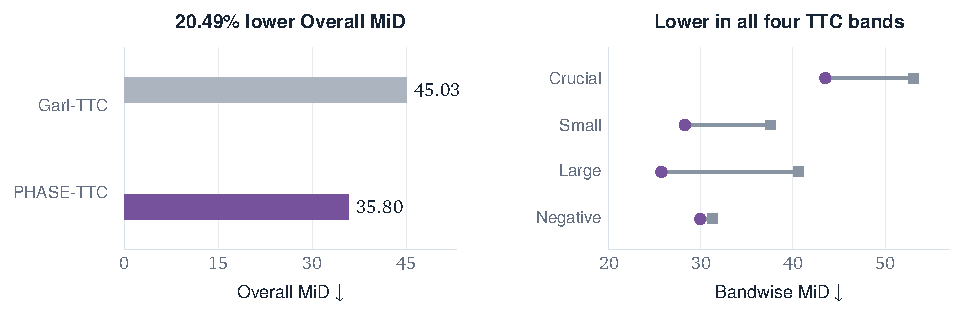
\includegraphics[width=\linewidth]{figures/rev_hero.pdf}
\caption{\textbf{GarlTTC Test leaderboard, 28 October 2026.} Overall MiD appears on the left and the four TTC bands on the right. Circles denote PHASE-TTC and squares Garl-TTC. Both entries report 0\% scorer-defined failures across 6,762 tokens. \evidence{B01,B02}}
\label{fig:official}
\end{figure}
\clearpage
\tableofcontents
\medskip
\finding{Evaluation overview}{\textbf{GarlTTC Test:} scored benchmark performance (6,762 tokens).\par
\textbf{Labeled EvTTC transfer:} errors and constituent controls (468 eligible queries).\par
\textbf{Unscored EvTTC competition:} coverage and disagreement (434 queries).\par
\textbf{Paced replay:} complete-output response time (250 updates).}
\clearpage
\section{Introduction}
An approaching object's image expands before contact. Recovering time-to-contact (TTC) from that expansion requires preserving small changes in scale through cropping, feature extraction, and temporal aggregation. Event cameras make this a particularly demanding measurement problem: they record asynchronous brightness changes, and the number of events depends on texture, illumination, contrast, and sensor thresholds as well as motion. Features that predict event activity accurately may therefore carry little information about approach speed.

PHASE-TTC combines geometric measurements from events and RGB images with their recent history. Each modality first produces its own motion estimate. The final fusion head receives named phase, timing, and support features and learns a correction to the RGB estimate. This lets the two branches share interpretable measurements without requiring their hidden coordinates to align. We train the later stages on out-of-fold predictions generated from separate sequence groups. \evidence{M22,M23}

The resulting TRAIN40 system ranks first on the public GarlTTC Test leaderboard as of 28 October 2026. It scores \OfficialPhasePublishedOverallMiD{} Overall MiD, compared with \OfficialGarlOverallMiD{} for Garl-TTC, with a 0\% scorer-defined failure rate over \OfficialSampleCount{} tokens \citep{codabench2026}. This \OfficialOverallRelativeGain{} reduction is measured in the benchmark's weighted phase error. To understand the result beyond the leaderboard, we examine the contribution of each modality, the effects of temporal context, and the time required to deliver a complete prediction. \evidence{B01,B02}

We also apply frozen checkpoints to 434 queries from ten EvTTC competition sequences. PHASE-TTC returns a prediction for every query; reproduced Garl full, event-only, and visual-only models return 424, 434, and 426 predictions. Verified TTC labels are not yet mapped to these exact queries. We therefore analyze coverage and disagreement between models, keeping this experiment separate from the earlier labeled transfer evaluation (Section~\ref{sec:evttc-competition}). \evidence{T01}

\subsection{Contributions}
Our contributions are the phase-based estimator and its training procedure, an evaluation that includes both modalities separately, and a study of prediction delivery under paced arrivals. The design experiments explain which changes helped and which failed. A post-hoc analysis compares fusion and RGB errors on the labeled transfer queries, with uncertainty estimated by resampling complete sequences (Appendix~\ref{app:derived-transfer}).

\subsection{Relation to prior work}
Event cameras provide high temporal resolution through asynchronous brightness changes, but downstream algorithms must still construct task-relevant spatial and temporal representations \citep{eventsurvey}. DSEC demonstrates synchronized event and frame acquisition in demanding driving conditions \citep{dsec}.

I-JEPA learns by predicting target representations from context \citep{ijepa}. VICReg regularizes representation variance and covariance \citep{vicreg}. These approaches motivate the early predictive-learning experiments, whose losses and regularizers are reported with each configuration.

Predictive joint embeddings can favor slowly varying distractors over a changing state of interest \citep{slowfeatures}. We test this possibility by changing nuisance dynamics independently of the TTC signal. The resulting controls help distinguish predictable appearance from useful motion information.

Prior event-based TTC methods estimate motion through geometric fitting and spatio-temporal registration \citep{eventaided}. EvTTC supplies synchronized observations and a dedicated TTC benchmark \citep{evttc}. The eAP study introduces geometry-aware representations for event-enhanced perception and the Garl models used in our comparisons \citep{eap}. We retain the evaluation populations defined by each experiment when comparing these methods. \evidence{T02}
\clearpage
\section{The final PHASE-TTC system}
\label{sec:train40}

\subsection{Deployed model composition}

PHASE-TTC deploys a causal chain of nine fitted components derived from the V16 PHASE-ONLY family: four modality-specific producers, two PAIR heads, two context refiners, and one fusion head. RGB and events each use an A5 baseline producer and a coarse-to-fine C2F producer. The PAIR readouts extract phase features from their A5 representations, after which the context refiners incorporate temporal history. The fusion head anchors its correction on the refined RGB estimate. Figure~\ref{fig:deployed-architecture} traces this path; the five auxiliary rotations serve training only. \evidence{M22,M23}

\begin{figure}[htbp]
  \centering
  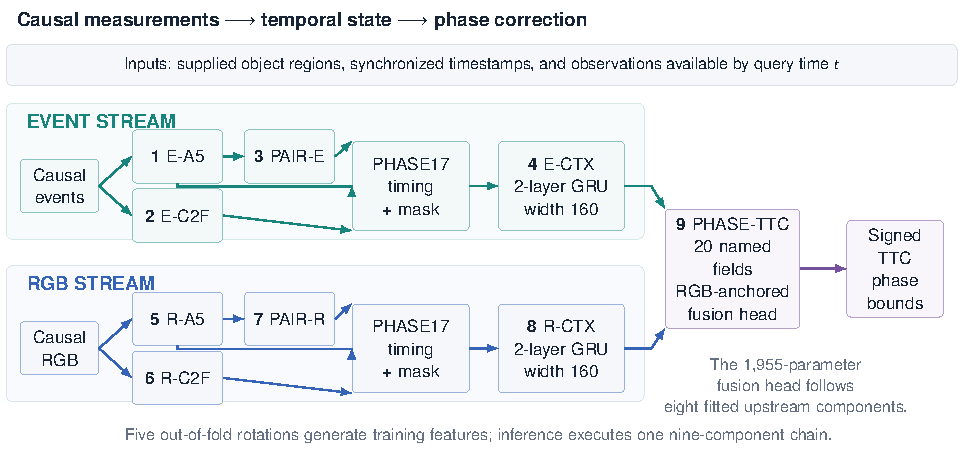
\includegraphics[width=\linewidth]{figures/rev_architecture.pdf}
  \caption{\textbf{Causal nine-component inference graph.} Supplied object regions feed parallel RGB and event producers, PAIR heads, and temporal refiners. Twenty named fields enter the final RGB-anchored fusion head. \evidence{M03,M22,M23}}
  \label{fig:deployed-architecture}
\end{figure}

Final fitting uses 88,744 TRAIN40 queries from forty sequences. The former P, H, and V groups all contribute to this refit, so their earlier scores characterize development rather than independent validation of the deployed chain. Each producer receives 49,932 updates, equivalent to eighteen epochs at effective batch size 32. The event producers carry forward the earlier TRAIN40 weights; RGB training resumes to the same endpoint. \evidence{L43}

\subsection{Object coordinates and causal history}

Each query includes supplied object coordinates. A common spatial frame covers both endpoint regions and preserves apparent scale change, which independent tight crops can erase. The evaluated system therefore assumes external localization. \evidence{M03}

Both branches use observations available by query time \(t\), with up to 650\,ms of causal history. Runtime begins at its declared measurement boundary and ends when the host receives the TTC output at \(t+L\). Figure~\ref{fig:causal-history} separates the sensing interval from response time; its observation marks are schematic. \evidence{M22,L43,L44}

\begin{figure}[H]
  \centering
  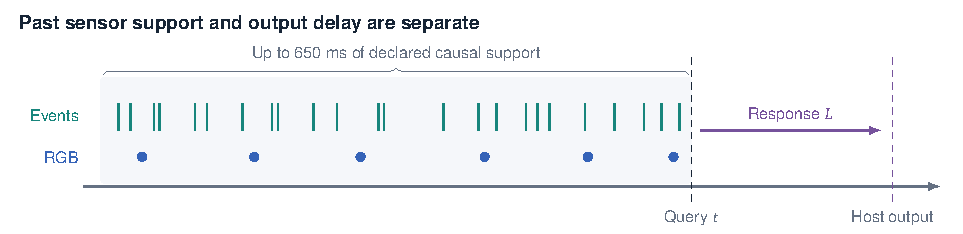
\includegraphics[width=\linewidth]{figures/rev_history.pdf}
  \caption{\textbf{Causal support and response-time boundaries.} RGB and event observations precede query time \(t\). The latency clock spans the declared runtime boundary to the complete host TTC output at \(t+L\).}
  \label{fig:causal-history}
\end{figure}

\subsection{Compact fusion interface}

Each context refiner is represented for final fusion by a constructed 170-coordinate block. Coordinates 0--159 are its learned hidden state. Coordinates 160--169 are an explicit interface containing, in order, one raw location, one emitted phase, three expert phases, four current timing values, and one valid-history count divided by eight. Concatenating the RGB block followed by the event block gives the 340-coordinate container
\begin{equation}
  \mathbf{s}=\left[\mathbf{s}_{R}^{170};\mathbf{s}_{E}^{170}\right]\in\mathbb{R}^{340}.
\end{equation}
Fusion reads \(\mathbf{s}_{160:170}\) and \(\mathbf{s}_{330:340}\), yielding twenty named phase, timing, and support inputs while the 160-dimensional hidden states remain within their modality branches. Within each ten-coordinate block, the first five phase coordinates are divided by \(0.03\); timing and support keep their native scaling. The shared interface aligns quantities with consistent meanings across the separately fitted refiners. \evidence{M22}

The selected vector passes through
\begin{equation}
  20\rightarrow 32\;[\mathrm{LayerNorm},\mathrm{SiLU}]
  \rightarrow 32\;[\mathrm{LayerNorm},\mathrm{SiLU}]
  \rightarrow 3.
\end{equation}
Zero initialization of the last affine layer makes the initial fusion output equal to the RGB anchor. If \(c_0,c_1,c_2\) are the three head outputs, \(\ell_R\) is the RGB raw-location anchor, and \(\mathbf{w}_R\) is the separately supplied pair of RGB width logits, the deployed computation is
\begin{align}
  \ell_F &= \ell_R + 0.03c_0, \\
  \boldsymbol{\sigma}_F &= 0.03\,\operatorname{softplus}\!\left(\mathbf{w}_R+[c_1,c_2]\right), \\
  \widehat{\mathrm{TTC}} &= \operatorname{phase\_to\_ttc}(\ell_F), \\
  q_{10}^{\phi} &= \operatorname{clip}(\ell_F-\sigma_{F,0},\,\phi_{\min},\phi_{\max}), \\
  q_{90}^{\phi} &= \operatorname{clip}(\ell_F+\sigma_{F,1},\,\phi_{\min},\phi_{\max}).
\end{align}
The native bounds are \(\phi_{\min}=-\log 2+10^{-6}\) and \(\phi_{\max}=8\). For the point prediction, the inverse map clamps \(\ell_F\) to these bounds, computes \(q=-\operatorname{expm1}(-\phi)/0.1\), and emits \(\operatorname{sgn}_{+}(q)/\max(|q|,1/60)\) seconds, where \(\operatorname{sgn}_{+}(0)=1\). Thus the emitted magnitude is at most 60\,s and zero phase maps to \(+60\)\,s. The reported point phase is recomputed from this finite TTC; the learned-width phase-interval endpoints are clamped separately. Saturation is a numerical convention, not a measured 60-second collision time or a calibration result. \evidence{M22,R02}

The compact fusion head contains 1,955 trainable parameters: \(672+64+1{,}056+64+99\) across three affine layers and two LayerNorms. Figure~\ref{fig:fusion-interface} summarizes the slicing and anchored output map. \evidence{M22}

\begin{figure}[htbp]
  \centering
  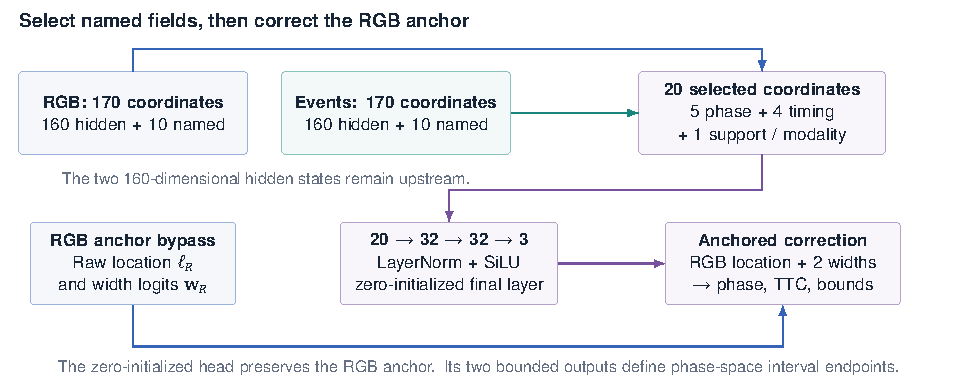
\includegraphics[width=\linewidth]{figures/rev_fusion.pdf}
  \caption{\textbf{Named-feature fusion interface.} Twenty phase, timing, and support coordinates are selected from the 340-value container. The RGB anchor and width logits follow a separate bypass into the three-output correction head. \evidence{M22}}
  \label{fig:fusion-interface}
\end{figure}

\subsection{Submission coverage and benchmark status}

The official submission contains finite predictions without fallback for 6,762 query tokens across twelve sequences: 5,805 physical queries and 957 aliases. Aliases identify repeated physical queries and do not represent additional inference work. \evidence{L44}

Section~\ref{sec:official} reports the official test result for this V16-derived PHASE-ONLY graph. The later V18 controls evaluate a different configuration. \evidence{B01,B02,L44}
\FloatBarrier
\section{Training and evaluation}
\label{sec:protocol}

\subsection{Grouped out-of-fold training and final refitting}

Five rotations of eight-sequence blocks generate leakage-controlled inputs for the upper stages. In each rotation, twenty-four groups fit the four producers and two PAIR heads, eight different groups fit the context refiners and normalizers, and the remaining eight groups generate out-of-fold features. A query group never contributes to supervised fitting of the models that generate its upper-stage features. \evidence{M23}

We pool PHASE17 RGB and event features across the out-of-fold rotations to train the context heads and normalizers. Those models then generate the PHASE20 features, expressed through the 340-coordinate container, for fusion-head training. Rotations pool named fields with shared semantics, while learned hidden coordinates stay within their originating models. Targets join the data only after out-of-fold feature generation. \evidence{M23}

\begin{figure}[htbp]
\centering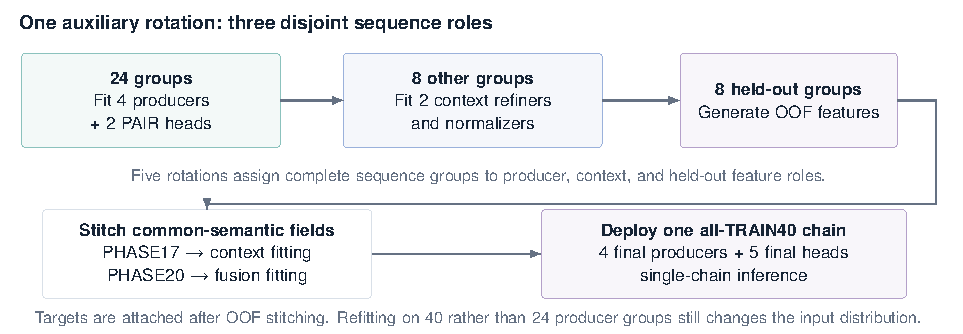
\includegraphics[width=\linewidth]{figures/rev_oof.pdf}
\caption{\textbf{Five-rotation fitting scheme.} Each rotation separates producer fitting, context fitting, and held-out feature generation. Final refitting produces one all-TRAIN40 inference chain. \evidence{M23}}
\label{fig:oof}
\end{figure}

Inference executes one all-TRAIN40 chain comprising the four producers, two PAIR heads, two context refiners, and fusion head. Auxiliary producers see twenty-four groups per rotation, whereas deployed producers see all forty. This stage-wise exposure difference can shift the upper-stage feature distribution after refitting. Earlier development use also remains relevant to architecture-selection claims.

Training comprised 690,934 auxiliary endpoint updates and 58,660 final-head updates across forty-five fits. Final PAIR endpoints used 11,264 updates; each context model and the final head used 12,044. Schedulers and warmup scaled with the fitting population. Update counts describe optimization exposure rather than wall-clock GPU effort. \evidence{L45}

Producer training combines relational DINO teacher signals, foreground geometry supervision, and task-specific adaptation. The deployed chain no longer evaluates the generic teacher, but its supervision remains part of the training recipe.


\subsection{Metrics and target coordinates}
TTC error in seconds, inverse-TTC error, benchmark phase error, and detection of urgent risk measure different aspects of behaviour. We use the signed benchmark phase
\begin{equation}
\phi(T)=-\log\!\left(1-\frac{0.1\,\mathrm{s}}{T}\right),\qquad T<0\;\text{or}\;T>0.1\,\mathrm{s}.
\end{equation}
Negative TTC denotes recession. The interval $[0,0.1]$\,s is outside this transform's domain. The official benchmark scorer defines motion-in-depth (MiD) error as
\begin{equation}
 \mathrm{MiD}(\widehat T,T)=10^4\left|\log\left(1-\frac{0.1}{T}\right)
 -\log\left(1-\frac{0.1}{\widehat T}\right)\right|
 =10^4|\phi(\widehat T)-\phi(T)|.
\end{equation}
MiD measures phase displacement. At large positive $T$, the first-order approximation $\phi(T)\simeq0.1/T$ compresses differences in seconds, while sensitivity rises near the positive domain boundary. We therefore report MAE in seconds alongside MiD. \evidence{M10,M15}

The scorer groups target TTC into four right-closed intervals: crucial $c:(0,3]$\,s, small $s:(3,6]$\,s, large $l:(6,10]$\,s, and negative $n:(-10,0]$\,s. The grouping includes zero in the negative band, although the phase transform is undefined at zero; metric validity is checked separately. Targets outside these bands do not contribute to the band-weighted score.

The scorer computes the band-weighted score
\begin{equation}
 \mathrm{overall\_MiD}=0.5\,\mathrm{MiD}_{c}+0.3\,\mathrm{MiD}_{s}
                     +0.1\,\mathrm{MiD}_{l}+0.1\,\mathrm{MiD}_{n},
\end{equation}
and a sample-weighted mean MiD. Missing bands remain missing, without weight redistribution. The complete band-weighted score requires targets in all four bands. The evaluation fixes the scorer by SHA-256 and tests a perfect four-band example, a hand-computed crucial-band error, and an absent negative band. \evidence{M15}

Metric reductions retain failures explicitly. The wrapper records invalid predictions by band and leaves its strict mean unavailable when any row is invalid. The official failure rate differs from the false-negative rate for urgent collision warnings. We therefore report prediction coverage, invalid-MiD count, and risk recall with their respective metrics. A finite saturated TTC may still carry an unsupported-measurement flag.

\subsection{Official benchmark and exploratory evaluations}

\begin{table}[H]
\centering\small
\caption{Evaluation populations and the quantities each supports. Historical46 and Extended-new share three sequence groups but no query identities.}
\label{tab:evaluation-populations}
\begin{tabularx}{\linewidth}{@{}>{\raggedright\arraybackslash}p{.24\linewidth}>{\raggedright\arraybackslash}p{.22\linewidth}X@{}}
\toprule Population & Size & Interpretation \\\midrule
Official GarlTTC Test & 6,762 scored tokens & Private targets; band-weighted MiD and scorer-defined failures. \evidence{B01,B02} \\
Published Garl EvTTC & 3 sequences & Published RTE; target/query correspondence to our run unverified. \evidence{T02} \\
EvTTC competition & 434 queries; 10 sequences & Unscored predictions, coverage and disagreement. \evidence{T01} \\
EvTTC Extended-new & 468 targets; 32 sequences & Labeled, development-exposed transfer with annotated ROI. \evidence{L01} \\
EvTTC Historical46 & 46 targets; 3 sequences & Labeled, development-exposed transfer with annotated ROI. \evidence{L01} \\
\bottomrule\end{tabularx}
\end{table}

The official GarlTTC Test submission covers twelve sequences and uses TRAIN40 event--RGB inputs with up to 650\,ms of causal history. Section~\ref{sec:official} reports the public ranking as of 28 October 2026 over \OfficialSampleCount{} scored tokens, including aliases of repeated physical queries \citep{codabench2026}. The evaluator scores submitted TTC values without standardizing temporal support, localization, supervision, or runtime across systems. Separate development experiments probe mechanisms within their tested configurations. \evidence{B01,B02,L44}

\subsection{Independence and paired comparisons}
Complete sequences form the units of separation and resampling. A sample-weighted sequence bootstrap carries all rows from each sampled group into the replicate and recomputes the ratio of summed losses to summed counts; sequence-macro summaries weight groups equally. Both reductions inherit any development exposure. Appendix~\ref{app:evaluation-details} gives the corresponding lineage, causality, and latency checks. \evidence{M15--M20}

Three head seeds quantify optimization variability conditional on their parents; they do not independently replicate the upstream representation. The additional transfer bootstrap is post hoc: it resamples saved paired predictions without changing a model, split, or historical interval (Appendix~\ref{app:derived-transfer}).
\FloatBarrier
\FloatBarrier
\section{Official GarlTTC benchmark result}
\label{sec:official}

\subsection{Public ranking and bandwise accuracy}

As of 28 October 2026, PHASE-TTC ranks first among the three displayed submissions on the official GarlTTC Test leaderboard. Submission \OfficialPhaseSubmissionID{}, listed as \emph{PHASE-TTC (TRAIN40, 650 ms causal history)}, records Overall MiD \OfficialPhasePublishedOverallMiD{} over \OfficialSampleCount{} scored tokens with a 0\% scorer-defined failure rate. The next displayed score is \OfficialGarlOverallMiD{} for the Garl-TTC reference. \citep{codabench2026} \evidence{B01}

The scorer returns Overall MiD \OfficialPhaseOverallMiD{} at full precision, consistent with the rounded public entry. Relative to Garl-TTC's published \OfficialGarlOverallMiD{}, PHASE-TTC reduces the ranking metric by \OfficialOverallRelativeGain{}. All four TTC bands improve (Table~\ref{tab:official-benchmark}); the large positive-TTC band has the largest relative reduction and the negative band the smallest. Percentage reductions combine the unrounded PHASE-TTC values with Garl-TTC's published two-decimal scores. \evidence{B01,B02}

\begin{table}[H]
\centering\small
\caption{Official GarlTTC Test scores on 28 October 2026 (lower is better). PHASE-TTC scores are shown to four decimals and Garl-TTC at published precision. Relative reductions use unrounded PHASE-TTC scores. Both entries have 6,762 scored tokens and 0\% scorer-defined failures. \evidence{B01,B02}}
\label{tab:official-benchmark}
\begin{tabular}{lrrr}
\toprule
\textbf{Metric} & \textbf{PHASE-TTC} & \textbf{Garl-TTC} & \textbf{Decrease} \\
\midrule
Overall & 35.8015 & 45.03 & 20.49\% \\
Crucial & 43.5190 & 53.13 & 18.09\% \\
Small & 28.2568 & 37.58 & 24.81\% \\
Large & 25.7179 & 40.61 & 36.67\% \\
Negative & 29.9314 & 31.29 & 4.34\% \\
\bottomrule
\end{tabular}
\end{table}

\subsection{Where the weighted difference comes from}

For band $b$, the additive contribution is $w_b(\mathrm{MiD}^{\mathrm{Garl}}_b-\mathrm{MiD}^{\mathrm{PHASE}}_b)$. The crucial and small bands contribute \OfficialCrucialSmallContributionShare{} of the Overall difference under weights 0.5 and 0.3. The large band's 0.1 weight limits its contribution despite its larger relative reduction; the negative band contributes least.



\begin{figure}[H]
\centering
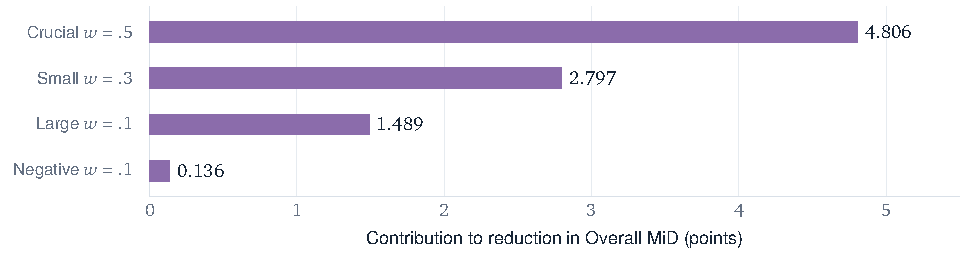
\includegraphics[width=.92\linewidth]{figures/rev_weighted.pdf}
\caption{\textbf{Bandwise contributions to the Overall MiD difference.} Crucial and small TTC account for about 82\% under the benchmark's $0.5/0.3/0.1/0.1$ weights. Table~\ref{tab:official-weighted-contributions} gives the rounding reconciliation. \evidence{B01,B02}}
\label{fig:official-weighted-contributions}
\end{figure}

\subsection{Metric and evaluation population}

The four TTC bands cover $(0,3]$, $(3,6]$, $(6,10]$, and $(-10,0]$ seconds. MiD measures error in the motion-in-depth coordinate defined in Section~\ref{sec:protocol}. The ranking uses the weighted Overall MiD; the scorer also reports \texttt{mean\_MiD}, an unweighted average over finite per-query errors. \citep{garlscorer2026}

The \OfficialSampleCount{} scored tokens represent 5,805 distinct physical queries and 957 aliases in the submitted package. Aliases reuse predictions at the same sensor query. The official failure criterion marks nonfinite TTC predictions or predictions with $|\widehat T|<0.1$\,s. Band scores average finite MiD values. The available aggregate outputs support bandwise analysis; studying individual errors requires per-query scores. \evidence{L44,B02}

\subsection{Scope of the comparison}

The submission declares RGB and event inputs, TRAIN40 fitting, and up to 650\,ms of causal history. Because the evaluator scores submitted TTC values, the leaderboard compares complete systems with their own temporal support, localization, supervision, and runtime choices. Section~\ref{sec:design-analysis} examines modality and temporal dependencies within the tested development configurations.

The official result measures the submitted system on private test targets. The exploratory EvTTC transfer compares frozen routes on development-exposed, positive-TTC sequences with annotated object regions. Section~\ref{sec:runtime} evaluates execution time separately, including deadline misses.
\FloatBarrier
\section{Frozen transfer and modality comparisons}
\label{sec:late-transfer}
\cohortline{LABELED TRANSFER / 468 eligible queries / 32 development-exposed sequences / annotated ROI}

On the labeled transfer queries, PHASE-TTC had lower error than the earlier Garl adapter, but the RGB-only model remained stronger on average. The full error distribution reveals a mixed comparison with RGB: fusion had a lower empirical 95th percentile and more of the largest errors.

\subsection{Evaluation data and scoring}

This evaluation uses labeled EvTTC sequences and the earlier frozen Garl adapter.
Both differ from the 434-query competition experiment in
Section~\ref{sec:evttc-competition}.

We froze the final candidate before evaluating transfer on EvTTC, with no further fitting or checkpoint selection. We registered sixteen uniformly spaced query times in each of thirty-two sequences with compatible sensors and object annotations, and retained forty-six queries from the earlier evaluation. Removing four duplicates left 554 physical queries. Predictions were fixed before using TTC labels for scoring. The selected query times differ from those in the earlier 946- and 3,640-query H8 evaluations, including on shared sequences.

Each query received the nearest public TTC label within 50\,ms, with the earlier timestamp breaking ties. Forty queries had no label within that tolerance. We scored Historical46 and Extended-new separately, using 46 and 468 labeled queries. Their query identities are disjoint after duplicate removal, although all three Historical46 sequences also appear among the thirty-two Extended-new sequences. All retained TTC labels are positive.

Relative time error was defined as
\begin{equation}
\mathrm{RTE}=100\,\frac{|\widehat T-T|}{|T|},
\end{equation}
without clipping the signed nonzero target. Pooled summaries give each query equal weight; sequence-macro summaries give each physical sequence equal weight. We resample whole sequences for confidence intervals to preserve correlation between nearby query times. EvTTC had already informed development, so the evaluation is exploratory. Inputs also use annotated boxes, and temporal support differs: PHASE-TTC can use up to 650\,ms, while Garl uses two frames and event segments separated by 0.1\,s. Both use float32 tensors, but backend settings were not matched.

\begin{table}[H]
\centering\small
\caption{Frozen TRAIN40 transfer on \texttt{extended\_new}: 468 GT-valid queries, 32 sequences, positive TTC only, annotated ROI. Pooled metrics; lower is better. Source \evidence{L01}.}
\label{tab:late-transfer}
\begin{tabular}{lrrrr}
\toprule
\textbf{Model} & \textbf{MAE (s)} & \textbf{RTE (\%)} & \textbf{Median AE (s)} & \textbf{P95 AE (s)} \\
\midrule
Event context & 1.451 & 65.70 & 0.857 & 4.397 \\
Garl reproduced & 3.258 & 140.07 & 0.674 & 5.252 \\
Phase correction & 1.023 & 41.23 & 0.464 & 3.243 \\
RGB context & 1.015 & 38.56 & 0.408 & 3.799 \\
\bottomrule
\end{tabular}
\end{table}



\subsection{Average error and the RGB comparison}

PHASE-TTC's advantage over the earlier Garl full adapter extended across most scenes: it had lower sequence-mean RTE on twenty-six of thirty-two Extended-new sequences. Its pooled RTE was 41.23\% and MAE 1.023\,s (Table~\ref{tab:late-transfer}). Giving each sequence equal weight produced an RTE difference of $-94.83$ percentage points, with a 95\% bootstrap interval of $[-210.50,-14.49]$. The wide interval reflects substantial variation across scenes. \evidence{L01}

RGB alone remained the stronger model on average, with RTE of 38.56\% and MAE of 1.015\,s on the same queries. It also had lower pooled errors on Historical46. The RGB branch is therefore a more demanding reference for assessing the value of event fusion than the earlier Garl adapter.

The ordering changes farther into the saved error distribution. RGB also has the lower median error, while fusion's empirical 95th percentile is 3.24\,s against RGB's 3.80\,s (Figure~\ref{fig:transfer-tradeoff}). Fusion has lower sequence-mean RTE on fourteen of thirty-two sequences (Figure~\ref{fig:transfer-sequence}). \evidence{L01,L46}

\begin{figure}[H]
\centering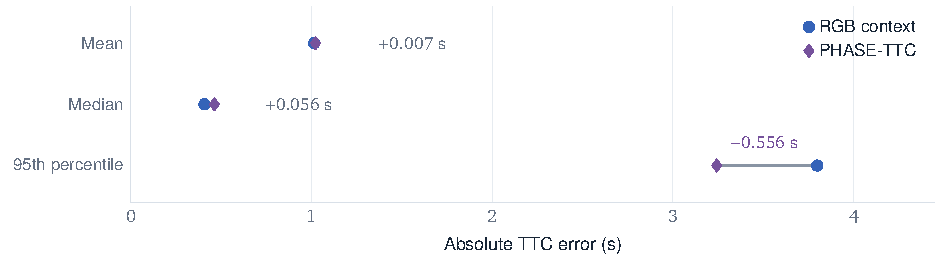
\includegraphics[width=0.94\linewidth]{figures/rev_transfer_pair.pdf}
\caption{\textbf{Absolute-error summaries for fusion and RGB.} Connected points compare the mean, median, and 95th percentile on the same 468 Extended-new queries. RGB has lower mean and median error; PHASE-TTC has a lower 95th percentile. Table~\ref{tab:revision-bootstrap} gives intervals for the paired differences.}
\label{fig:transfer-tradeoff}
\end{figure}

\subsection{Error exceedance and paired uncertainty}
The saved predictions contain fewer moderately large fusion errors but more extreme ones. PHASE-TTC has fewer absolute errors above 3\,s (29 versus 37) and 5\,s (9 versus 13), yet more above 10\,s (5 versus 2). Its maximum error reaches 32.5\,s, nearly twice RGB's 16.6\,s. We computed these threshold counts post hoc, retaining every eligible prediction in Figure~\ref{fig:transfer-exceedance}. \evidence{R01,L46}

\begin{figure}[htbp]
\centering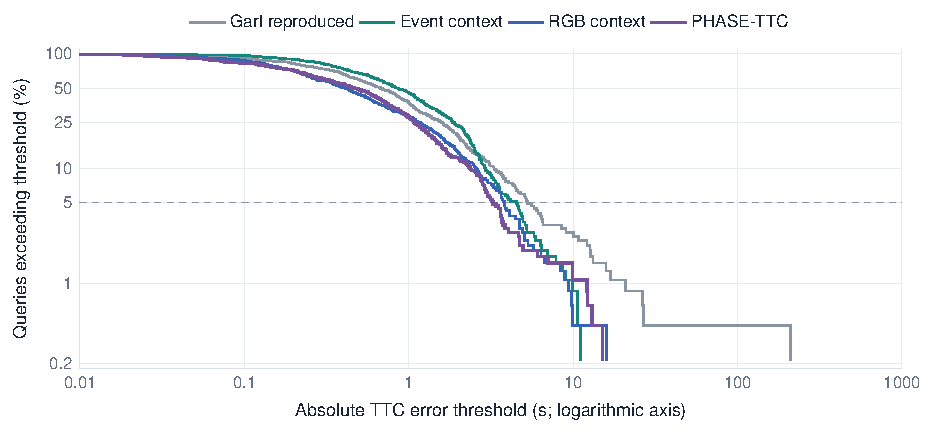
\includegraphics[width=\linewidth]{figures/rev_exceedance.pdf}
\caption{\textbf{Fraction of queries exceeding each absolute-error threshold.} Curves use all 468 labeled queries, with equal query weights and logarithmic axes. The dashed line marks 5\%. The plotted range includes the earlier Garl adapter's outlier above 600\,s. \evidence{R01,L46}}
\label{fig:transfer-exceedance}
\end{figure}

Resampling complete sequences gives a PHASE-minus-RGB p95 difference of $\RevisionPninetyfiveDelta$\,s, with a 95\% interval of $[\RevisionPninetyfiveLow,\RevisionPninetyfiveHigh]$\,s. The mean and median difference intervals also include zero. These exploratory intervals use 10,000 paired replicates, a fixed seed, and linear quantiles; they describe the saved models on sequences already used during development. Appendix~\ref{app:derived-transfer} provides the procedure, every sequence result, and two numerical cases selected post hoc. \evidence{R01}
\begin{table}[H]\centering\small
\caption{Paired differences in absolute error across 468 labeled queries from 32 sequences. Percentile intervals use 10,000 paired sequence resamples. \evidence{R01; derived from L46}}
\label{tab:revision-bootstrap}
\begin{tabular}{@{}lrrr@{}}\toprule
Metric & RGB (s) & PHASE-TTC (s) & Difference [95\% interval] (s)\\\midrule
Mean absolute error & 1.015 & 1.023 & $+0.007\;[-0.110,+0.129]$ \\
Median absolute error & 0.408 & 0.464 & $+0.056\;[-0.038,+0.145]$ \\
95th percentile & 3.799 & 3.243 & $-0.556\;[-1.126,+0.241]$ \\
\bottomrule\end{tabular}
\end{table}




\FloatBarrier
\section{Unscored competition inputs: coverage and disagreement}
\label{sec:evttc-competition}
\cohortline{UNSCORED INFERENCE / 434 query identities / 10 sequences / coverage and prediction disagreement}
We applied three released Garl-TTC variants to the same ten-sequence EvTTC inputs as the frozen PHASE-TTC reference. The 434 queries span eight road and two Slider sequences, with sequence, row, frame index, and timestamp matched across models. The comparison contains 1,302 Garl outputs and 434 PHASE-TTC outputs. \evidence{T01}

No verified numeric TTC targets map to these 434 query identities. We therefore measure coverage and paired prediction disagreement:
\begin{equation}
d_i^{(m)}=\widehat T_{i,m}^{\rm Garl}-\widehat T_i^{\rm PHASE},\qquad a_i^{(m)}=|d_i^{(m)}|.
\label{eq:evttc-disagreement}
\end{equation}
The differences in Equation~\ref{eq:evttc-disagreement} compare model outputs rather than prediction error. This population differs from both the labeled transfer in Section~\ref{sec:late-transfer} and Garl's published three-sequence RTE evaluation. Appendix~\ref{app:competition-details} gives the adapter, timing measurements, and ten sequence traces.

\subsection{Frozen checkpoints and native input support}
The released full, event-only, and visual-only state dictionaries load strictly and run in float32 with frozen weights. RGB-dependent routes use two real causal frames, while event-only uses two observed causal intervals. Startup queries without the required observations remain unavailable. PHASE-TTC uses up to 650\,ms of context, so the models share query identities under different temporal support. \evidence{T01}

Supplied boxes and calibration condition each route. Rotation-only projection omits translation because object depth is unavailable. For Slider, the adapter derives rotation from the supplied camera poses because the data provide no named event-to-RGB extrinsic. We treat the resulting runs as frozen-checkpoint adaptations.

\subsection{Coverage, sign, and disagreement tails}
\begin{table}[tbp]
\centering\small
\caption{Predictions on 434 EvTTC competition queries. The table reports finite-output coverage, signed TTC range, and negative counts. Median and P95 summarize absolute differences from PHASE-TTC where both models produce finite outputs. \evidence{T01}}
\label{tab:evttc-model-summary}
\begin{tabular}{@{}lrrrrr@{}}
\toprule
\textbf{Model} & \textbf{Finite} & \textbf{Range (s)} & \textbf{$<0$} & \textbf{Median (s)} & \textbf{P95 (s)} \\
\midrule
PHASE-TTC & 434/434 & [-42.225, 51.869] & 2 & -- & -- \\
Garl full & 424/434 & [0.907, 52.705] & 0 & 0.261 & 1.098 \\
Garl event-only & 434/434 & [-42.211, 406.095] & 10 & 0.681 & 5.623 \\
Garl visual-only & 426/434 & [-23.832, 38.767] & 5 & 0.236 & 1.524 \\
\bottomrule
\end{tabular}
\end{table}
PHASE-TTC and event-only Garl each emit 434 finite values; full Garl emits 424 and visual-only 426. The first query in each road sequence lacks two causal RGB frames, creating eight gaps in both RGB-dependent variants. Full Garl has two further Slider-750 gaps because the earlier event endpoint precedes recorded coverage. All invoked models return finite values; nulls correspond to unavailable inputs.

\begin{figure}[htbp]
\centering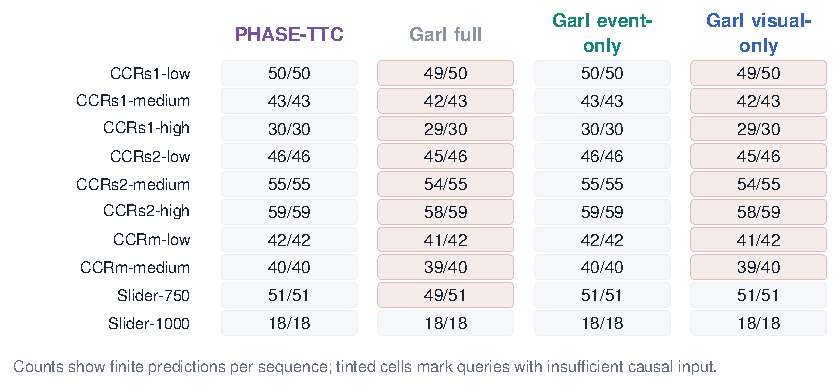
\includegraphics[width=\linewidth]{figures/rev_coverage.pdf}
\caption{\textbf{Finite prediction coverage by model and sequence.} Tinted cells mark the eight missing road RGB pairs and two additional early Slider-750 event gaps in full Garl. \evidence{T01}}
\label{fig:evttc-coverage}
\end{figure}

On shared finite rows, median absolute disagreement from PHASE-TTC is 0.26\,s for full Garl, 0.68\,s for event-only, and 0.24\,s for visual-only. Their p95 disagreements are 1.10, 5.62, and 1.52\,s. Full Garl emits no negative TTC, compared with two negative PHASE-TTC outputs, ten event-only outputs, and five visual-only outputs. \evidence{T01}

Slider-750 contains the largest excursions: event-only reaches 406.10\,s, with p95 absolute disagreement of 241.68\,s. The native height-ratio conversion becomes ill-conditioned as the two predicted endpoint heights approach equality. Figures~\ref{fig:evttc-predictions-symlog} and~\ref{fig:evttc-predictions-linear} preserve the sign and magnitude of these outputs across all ten sequences. \evidence{T01}

Timing remains descriptive because the variants ran once in fixed order with shared cache and warm-state effects, and PHASE-TTC used a different adapter and longer history. \evidence{T01}
\FloatBarrier
\section{Design analysis and controlled ablations}
\label{sec:design-analysis}
Three findings shaped PHASE-TTC: preserving scale change mattered more than representation stability alone; correcting an expert's phase could improve on selecting an expert; and changing the loss often traded one TTC range against another. The studies below used different data splits and pretrained models. Appendices~\ref{sec:early}, \ref{sec:temporal-recovery}, and~\ref{sec:late} give the full configurations and unsuccessful variants.

\subsection{Preserve the motion variable before predicting it}
Using a common object region preserves apparent expansion across observations. Independently resizing each endpoint can remove that signal before the network sees it (Figure~\ref{fig:crop}). An explicit object query also distinguishes objects that share one full-frame input but have different TTC targets. The estimator consequently requires externally supplied localization. \evidence{M03}

The synthetic experiments showed why embedding stability alone was insufficient. With slowly changing nuisance features, a temporal-residual objective recovered more dynamic information than a variance regularizer. Changing those nuisance features independently every frame reversed the ordering. The geometry experiments exposed a related difficulty: stable foreground maps and accurate absolute heights did not ensure accurate changes in scale. Some models also received RGB-derived SAM masks or DINOv3 relations during training, even when their inference inputs contained only events. \evidence{E02,E12,E25,E26}

Removing paths from a trained V8 model identified which inputs its prediction used. Analytic scale alone scored 373.18 MiD, and adding the residual without transport gave 373.60. Restoring transport reduced the score to 163.23; restoring history reduced it further to 155.82. The weights remained fixed throughout these tests. Separate JEPA controls did not establish a benefit from predictive pretraining. \evidence{E21,E23,E24}

\subsection{Correct phase rather than only selecting an expert}
A hard router is limited to the predictions its experts already make. SIMPLEX-T can move beyond them by learning a correction around their median phase from masked temporal context. The auxiliary cost head still describes the original experts, so it does not directly estimate the corrected prediction's risk. The phase quantiles likewise require calibration before they can be interpreted as collision probabilities. \evidence{M_TEMPORAL_MODEL,M_PHASE_CONTRACT}

Extending history from H8 to H16 lowered MiD for each of three head seeds on OLD\_DEV. The paired interval across all seeds excludes zero. However, one seed had already informed exploration; the two new seeds alone give a difference of $-2.42$ MiD with interval $[-5.24,0.04]$. All heads shared the same upstream producers. Figure~\ref{fig:main-h16} shows both summaries; H8 remained the selected candidate. \evidence{M_SIMPLEX}
\begin{figure}[htbp]
\centering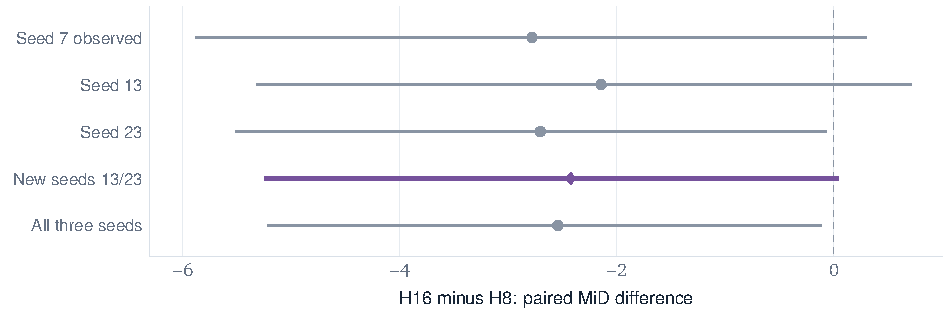
\includegraphics[width=.97\linewidth]{figures/rev_h16.pdf}
\caption{\textbf{H16 minus H8 on nine OLD\_DEV sequences.} Points show paired MiD differences and lines show the recorded hierarchical 95\% intervals. The highlighted estimate uses only the two new head seeds; its interval includes zero. \evidence{M_SIMPLEX}}
\label{fig:main-h16}
\end{figure}

Keeping all experts produced the lowest score in the removal study: FULL-C0 reached 121.40 MiD, compared with 127.79 for A5-only, 126.70 for C2F-only, and 124.67 for A5 plus PAIR. \evidence{M_SIMPLEX}

In the temporal-aggregation comparison, set aggregation with age gave 122.44 MiD; removing explicit time gave 123.69. Because the frozen experts can already encode temporal information, the remaining differences cannot be assigned to recurrence alone. \evidence{M_X05}

Transport probes improved on destructive controls, but stronger calibrated or pooled alternatives narrowed that advantage. \evidence{M_STAGE61,M_STAGE62}

\subsection{Adaptation trades error between TTC ranges}
Changes to the readout often improved imminent-contact estimates at the expense of receding motion. V14 M1--L0 reduced crucial MiD from 156.83 to 134.47 but increased negative MiD from 61.38 to 84.21. V17's geometry bypass lowered the aggregate score on the development-used V split from 106.545 to 102.762 while worsening MAE; its head seeds shared encoders. Across V14--V17, loss reweighting, residual range, sampling, numerical precision, clipping, geometry bypasses, and height readouts failed to meet all acceptance criteria. Invalid height-derived predictions were retained in scoring. The next experiments therefore allowed the measurement model itself to adapt. \evidence{L02,L50--L52}

V18 full adaptation reduced aggregate MiD on H from 112.29 to 78.92 and crucial MiD from 157.27 to 95.85, while negative MiD rose from 65.52 to 87.09. The model passed the overall sign criterion but remained inaccurate in the magnitude of receding TTC. V19 increased the training weight on negative targets and recovered some negative-range accuracy and MAE, at the cost of aggregate and crucial-range error. \evidence{L10,L24,L25,L30}

\subsection{Events help in the matched V18 comparison}
Supplying real events improved V18 C1 relative to its equal-capacity ZERO control. TRUE-event fusion achieved aggregate MiD $87.29\pm0.87$, compared with $92.47\pm0.16$; dispersion is the sample standard deviation of the scalar scores across seeds. The paired comparison over complete groups also favored TRUE. Each seed repeated C1 adaptation and head fitting from the same A5 initialization and RGB context model. This experiment uses V18 C1, whereas the final TRAIN40 system derives from V16. \evidence{L03,L31--L33}
\begin{figure}[htbp]
\centering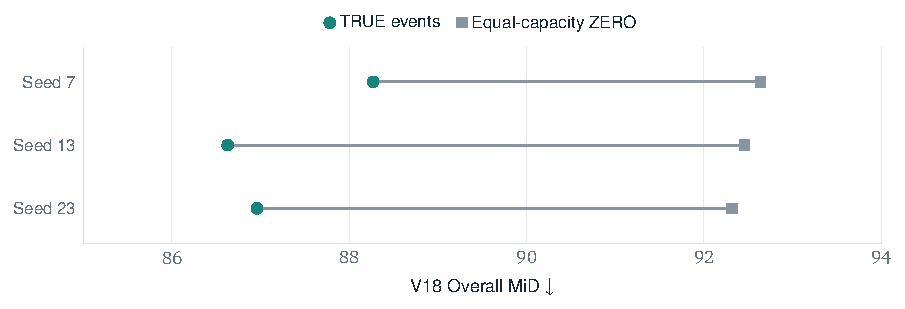
\includegraphics[width=.97\linewidth]{figures/rev_v18.pdf}
\caption{\textbf{Real versus zeroed events in V18 C1.} Each line pairs TRUE and ZERO scores for one adaptation/head seed. The models share the A5 initialization and RGB context model, and TRUE uses the observed event features. \evidence{L03}}
\label{fig:main-v18}
\end{figure}

The V18 crucial-band gain remained below its registered threshold. Its comparison with the preserved V16 model gave an interval of approximately $[-3.69,0.14]$, and no V18 candidate met all acceptance criteria. Testing ZERO events and equal temporal support in the final TRAIN40 recipe would be needed to extend the attribution result to the submitted system.
\FloatBarrier
\section{Runtime and causal service}
\label{sec:runtime}

The persistent service completed every update in its five-second paced replay and preserved numerical parity, but it missed the 20\,ms response target. The 95th percentile was 29.14\,ms. The distinction between model execution and delivery of a complete prediction explains why a faster inner kernel is not enough to meet the deadline.

\begin{figure}[H]
\centering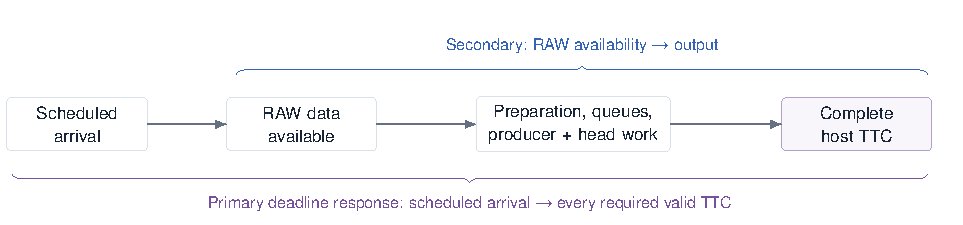
\includegraphics[width=\linewidth]{figures/rev_runtime_clock.pdf}
\caption{\textbf{Response clocks for one query.} Deadline response starts at scheduled arrival; the secondary clock starts when RAW data become available. Both stop when all required TTC outputs reach the host.}
\label{fig:runtime-clocks}
\end{figure}

\subsection{Latency measurement boundaries}

Earlier timing experiments measured different parts of the computation. V18 used warm raw-sensor queries with its original producer batching. The final test12 diagnostics timed a prepared eager path, and the EvTTC transfer measured adapter wall time, including preparation and cache behavior. Hardware and inputs also varied. We report these measurements separately and use the scheduled-arrival clock for the deadline test below. The saved timing record contains aggregate statistics, so the analysis uses quantiles and deadline counts rather than reconstructing a per-arrival distribution.

The service reduced repeated work by preparing RGB within the object region, extending event prefixes incrementally, and reusing reverse-transport summaries exactly. It also combined top-$k$ normalization with native query graphs and parallel branches, overlapping event execution with RGB preparation. RGB features were reused; event encodings were recomputed. A separate diagnostic verified all 462 recorded calls to the prepared transport component. \evidence{L41}

Numerical checks rejected several faster alternatives. Compiled transport arithmetic changed the final TTC on sensitive examples despite agreeing on most others. Processing smaller event packets preserved the tested state buffers, representations, and final predictions, but that experiment did not time the computation or run a 200\,Hz source through the paced service. It established a viable numerical path for a later timing experiment. \evidence{L42}

\subsection{Paced-service latency at 50 Hz}

We ran the replay on an NVIDIA GeForce RTX 5070 Ti Laptop GPU using Python 3.11.15 and PyTorch 2.11.0+cu128, built with CUDA 12.8. Computation used FP32 with TF32 disabled, two PyTorch CPU threads, eight RGB preparation workers, and a queue capacity of two. Model loading, synthetic shape priming, and initialization from preceding history finished before measured arrivals. Table~\ref{tab:runtime-setup} gives these setup intervals and the parity tolerance. \evidence{L40,R02}

The five-second replay processed 250 single-object updates from preloaded RAW data accessible only to the CPU feeder. All updates completed with zero drops and zero source errors, and independent post-run checks confirmed TTC parity. Nevertheless, 200 scheduled arrivals found earlier work unfinished. Of the 250 responses, 201 met or exceeded 20\,ms. Scheduled-arrival latency reached 29.14\,ms at p95, 32.41\,ms at p99, and 35.33\,ms at maximum. Starting the clock after RAW data became available gave a lower p95 of 25.25\,ms. \evidence{L40}

The measurement excludes disk I/O and covers one object over five seconds. It therefore leaves physical-camera input, sixty-second operation, and larger object counts for further testing. Failed replays remain in separate reports, including dropped updates and rapid error acknowledgements. We count latency only for successful TTC outputs, so a fast acknowledgement cannot improve the prediction-latency summary.

\begin{figure}[t]
\centering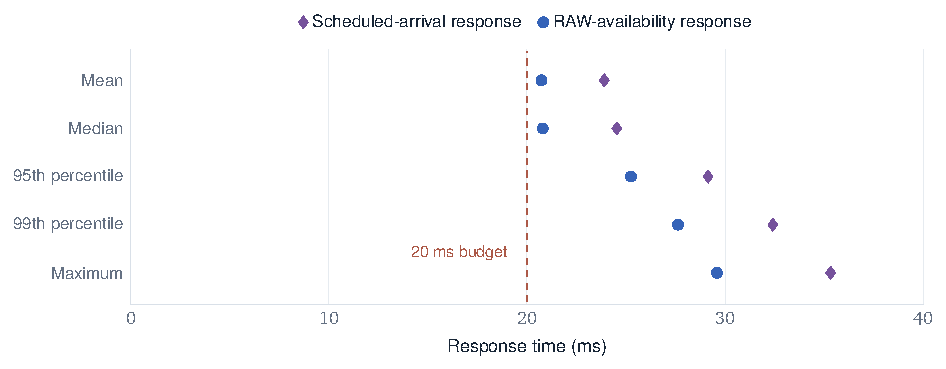
\includegraphics[width=0.98\linewidth]{figures/rev_runtime.pdf}
\caption{\textbf{Response-time summaries for 250 completed updates.} Scheduled-arrival latency has a p95 of 29.14\,ms. Of the 250 responses, 201 (80.4\%) meet or exceed 20\,ms. The second clock begins when RAW data become available. \evidence{L40}}
\end{figure}
\FloatBarrier
\section{Discussion and limitations}
\subsection{What the benchmark result establishes}
The official ranking shows that the submitted PHASE-TTC system performs well on GarlTTC Test. Its fusion head operates on phase, timing, and support features whose meanings remain comparable across the two modalities. This avoids requiring independently trained hidden coordinates to align. The ranking alone cannot determine how much of the gain comes from that interface, the longer history, or the upstream models; those questions require matched comparisons. \evidence{M22,M23}

The out-of-fold training procedure addresses a narrower problem: later stages should not train on features produced by a model fitted to the same sequence group. At deployment, however, they receive features from producers trained on all 40 groups rather than the 24 used in each auxiliary fit. That shift remains, as does the exposure involved in earlier architecture selection. The JEPA experiments provide a separate result: they did not establish a benefit from predictive pretraining, even when embeddings retained variance and effective rank. Subsequent supervised or teacher-assisted gains do not resolve that question.

\subsection{Where fusion helps, and where it fails}
The labeled transfer experiment gives a mixed answer about adding events. Fusion has a lower empirical p95 absolute error than RGB alone, but a higher mean and more errors above ten seconds. All three paired intervals for mean, median, and p95 differences include zero. \evidence{L01,L02,L30,R01}

The range experiments reinforce this point. Improving imminent-contact predictions sometimes worsened estimates for receding objects, because phase error, error in seconds, and warning behavior emphasize different parts of the problem. The labeled transfer includes only positive TTC and cannot test the full signed domain or a complete warning policy.

The 434-query competition experiment answers a different question. It establishes prediction coverage and disagreement between models, but verified TTC labels are not mapped to those exact queries. Its Garl visual-only checkpoint also differs from PHASE-TTC's RGB context model. Matching scenario names is insufficient to combine these results with the labeled transfer; the recordings and query identities must match as well. \evidence{T01,T02}

\subsection{Generalization and deployment}
Most development comparisons reuse sequences or upstream models. Repeating the head with different seeds measures variation conditional on those models, and nearby windows remain correlated observations of the same scene. Independent retraining and new sequences would test how much of the observed performance survives beyond these choices. Deployment also requires obtaining object regions causally; the current evaluations supply them, and rotation-only projection between sensors approximates alignment without depth.

The compact head has 1,955 parameters, but the full system includes all upstream components. A complete parameter and peak-memory inventory remains to be reported. The paced-run records specify the GPU, software, execution settings, and initialization excluded from timing, while omitting the CPU model and GPU driver version. Learned phase widths and propagated variances likewise need empirical calibration before they can support probability statements.

The runtime study identifies an operational bottleneck: all predictions remain numerically consistent, yet their p95 response exceeds 20\,ms. Input preparation and scheduling must improve along with kernel speed. A longer run with physical-camera input and multiple objects would test whether those improvements hold under sustained load. \evidence{L40--L42}

\section{Conclusion}
PHASE-TTC combines geometric measurements and recent history from events and RGB images, then corrects the RGB estimate through a compact phase-based head. It ranks first on the public GarlTTC Test leaderboard as of 28 October 2026, reducing Overall MiD by \OfficialOverallRelativeGain{} relative to Garl-TTC. The broader experiments show where further progress is needed: on the labeled transfer set, fusion trades a lower p95 against worse extreme errors; the competition predictions still need verified labels; and the paced service exceeds its deadline. Improving rare-error behavior and meeting sustained response deadlines remain central challenges for deployment.
\FloatBarrier
\clearpage
\begingroup\small
\setlength{\bibsep}{3pt}

\begin{thebibliography}{11}
\providecommand{\natexlab}[1]{#1}
\providecommand{\url}[1]{\texttt{#1}}
\expandafter\ifx\csname urlstyle\endcsname\relax
  \providecommand{\doi}[1]{doi: #1}\else
  \providecommand{\doi}{doi: \begingroup \urlstyle{rm}\Url}\fi

\bibitem[Assran et~al.(2023)Assran, Duval, Misra, Bojanowski, Vincent, Rabbat,
  LeCun, and Ballas]{ijepa}
Mahmoud Assran, Quentin Duval, Ishan Misra, Piotr Bojanowski, Pascal Vincent,
  Michael Rabbat, Yann LeCun, and Nicolas Ballas.
\newblock Self-supervised learning from images with a joint-embedding
  predictive architecture.
\newblock \emph{arXiv:2301.08243}, 2023.
\newblock URL \url{https://arxiv.org/abs/2301.08243}.

\bibitem[Bardes et~al.(2022)Bardes, Ponce, and LeCun]{vicreg}
Adrien Bardes, Jean Ponce, and Yann LeCun.
\newblock Vicreg: Variance-invariance-covariance regularization for
  self-supervised learning.
\newblock In \emph{ICLR}, 2022.
\newblock URL \url{https://arxiv.org/abs/2105.04906}.

\bibitem[Gallego et~al.(2020)Gallego, Delbruck, Orchard, et~al.]{eventsurvey}
Guillermo Gallego, Tobi Delbruck, Garrick Orchard, et~al.
\newblock Event-based vision: A survey.
\newblock \emph{IEEE Transactions on Pattern Analysis and Machine
  Intelligence}, 2020.
\newblock URL \url{https://arxiv.org/abs/1904.08405}.

\bibitem[{GarlTTC Benchmark}(2026)]{codabench2026}
{GarlTTC Benchmark}.
\newblock {GarlTTC Test public leaderboard}.
\newblock \url{https://www.codabench.org/competitions/17289/}, 2026.
\newblock Accessed 28 October 2026. PHASE-TTC submission 1016512.

\bibitem[Gehrig et~al.(2021)Gehrig, Aarents, Gehrig, and Scaramuzza]{dsec}
Mathias Gehrig, Willem Aarents, Daniel Gehrig, and Davide Scaramuzza.
\newblock Dsec: A stereo event camera dataset for driving scenarios.
\newblock \emph{IEEE Robotics and Automation Letters}, 2021.
\newblock URL \url{https://arxiv.org/abs/2103.06011}.

\bibitem[Li et~al.(2024)Li, Liao, Lu, Liu, Shen, and Zhou]{eventaided}
Jinghang Li, Bangyan Liao, Xiuyuan Lu, Peidong Liu, Shaojie Shen, and Yi~Zhou.
\newblock Event-aided time-to-collision estimation for autonomous driving.
\newblock In \emph{ECCV}, 2024.
\newblock URL
  \url{https://www.ecva.net/papers/eccv_2024/papers_ECCV/papers/07043.pdf}.

\bibitem[Li et~al.(2026)Li, Li, Lian, Li, Chen, and Zhou]{eap}
Jinghang Li, Shichao Li, Qing Lian, Peiliang Li, Xiaozhi Chen, and Yi~Zhou.
\newblock Toward deep representation learning for event-enhanced visual
  autonomous perception: the eap dataset.
\newblock \emph{arXiv:2603.16303}, 2026.
\newblock URL \url{https://arxiv.org/abs/2603.16303}.

\bibitem[{NAIL-HNU}(2026)]{garlscorer2026}
{NAIL-HNU}.
\newblock {Garl-TTC official benchmark evaluator}.
\newblock
  \url{https://github.com/NAIL-HNU/Garl-TTC/blob/main/garl_ttc_benchmark/codabench/scoring_program/score.py},
  2026.
\newblock Accessed 28 October 2026.

\bibitem[Sim{\'e}oni et~al.(2025)Sim{\'e}oni, Vo, Seitzer, Baldassarre, Oquab,
  et~al.]{dinov3}
Oriane Sim{\'e}oni, Huy~V. Vo, Maximilian Seitzer, Federico Baldassarre, Maxime
  Oquab, et~al.
\newblock Dinov3.
\newblock \emph{arXiv:2508.10104}, 2025.
\newblock URL \url{https://arxiv.org/abs/2508.10104}.

\bibitem[Sobal et~al.(2022)]{slowfeatures}
Vlad Sobal et~al.
\newblock Joint embedding predictive architectures focus on slow features.
\newblock \emph{arXiv:2211.10831}, 2022.
\newblock URL \url{https://arxiv.org/abs/2211.10831}.

\bibitem[Sun et~al.(2025)Sun, Li, Dai, Liao, Xiong, and Zhou]{evttc}
Kaizhen Sun, Jinghang Li, Kuan Dai, Bangyan Liao, Wei Xiong, and Yi~Zhou.
\newblock Evttc: An event camera dataset for time-to-collision estimation.
\newblock \emph{IEEE Robotics and Automation Letters}, 2025.
\newblock URL \url{https://arxiv.org/abs/2412.05053}.

\end{thebibliography}

\endgroup
\appendixdivider
\appendix
\section{Technical foundations and historical method families}
\label{sec:methods}

PHASE-TTC grew through four model families: predictive embedding, geometry-constrained endpoint estimation, phase-domain temporal refinement, and RGB-anchored event fusion. Each family tests a different mechanism with its own objective and inference path. \evidence{M01--M14}

\begin{figure}[H]
\centering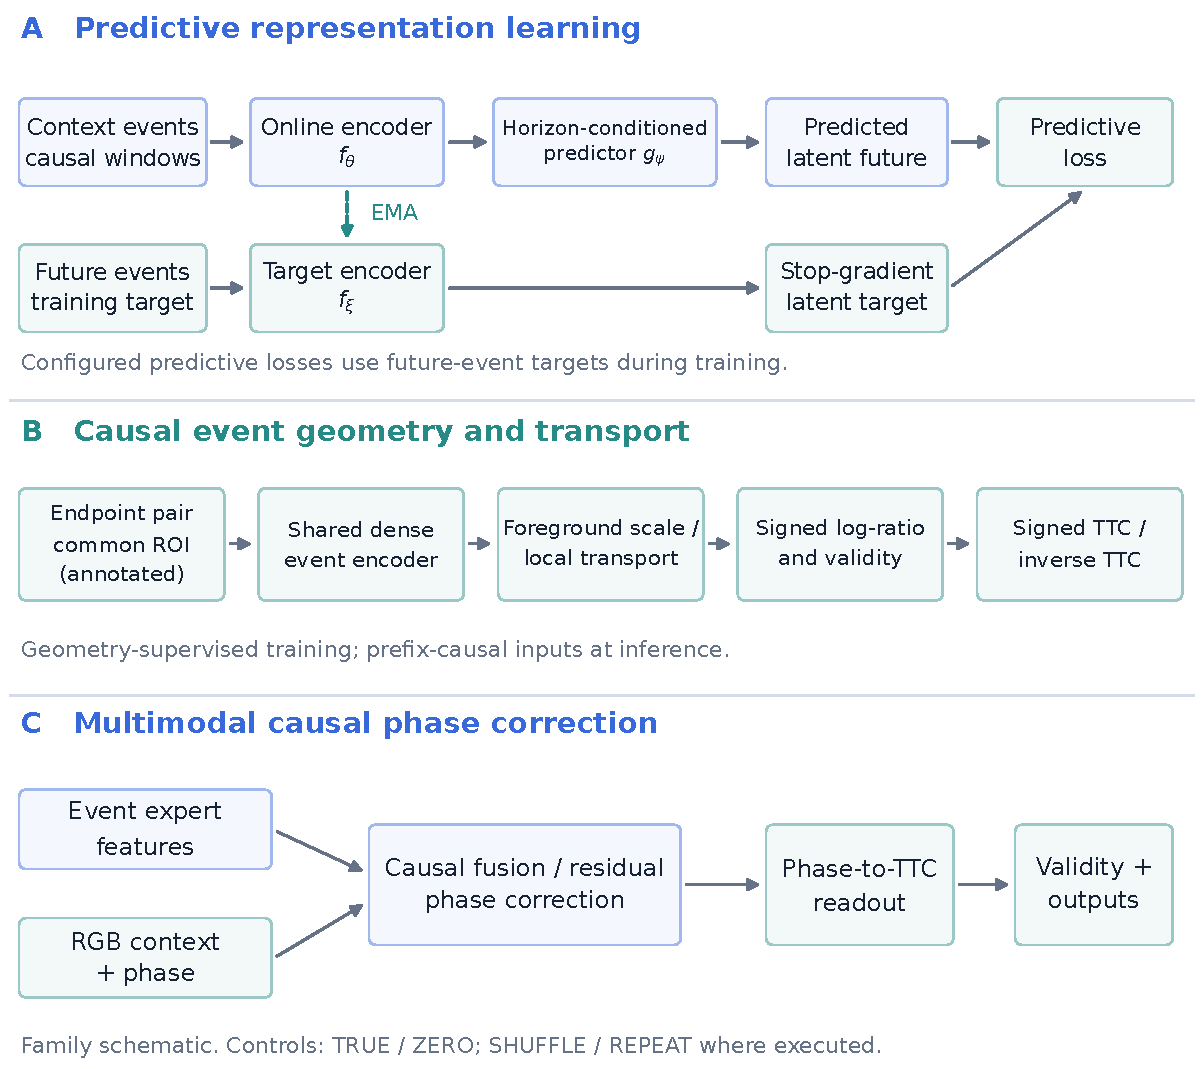
\includegraphics[width=\linewidth,height=.80\textheight,keepaspectratio]{figures/architecture.pdf}
\caption{\textbf{Selected model families.} (A) Predictive latent learning uses a training-only target branch. (B) Causal scale and transport map endpoint geometry to signed motion. (C) Phase-domain fusion combines event and RGB evidence. Panel A contains the JEPA objective; Sections~\ref{sec:phase-refinement} and~\ref{sec:train40} detail the later temporal and fusion paths.}
\label{fig:architecture}
\end{figure}
\FloatBarrier

\subsection{Events, temporal windows, and object coordinates}
An event stream is a sequence $\mathcal E=\{(x_i,y_i,t_i,p_i)\}_{i=1}^N$, with integer microsecond timestamps and normalized polarity $p_i\in\{-1,+1\}$. \texttt{EventBatch} stores aligned NumPy arrays for these fields. Each context window is anchored at its end time. Indexing rejects nonpositive durations, mismatched reference times, and future windows that begin before context ends. Causality tests cover crops, features, checkpoints, and calibration inputs. \evidence{M01}

The dense voxel representation distributes an event between adjacent temporal bins. For $K$ bins, duration $\Delta t$, and normalized time $u_i=(K-1)(t_i-t_0)/\Delta t$, the unnormalized representation is
\begin{equation}
 V_{p,k}(x,y)=\sum_i \mathbf 1[x_i=x,y_i=y,p_i=p]\max(0,1-|u_i-k|).
\end{equation}
Separate polarity yields $2K$ channels. Two flattened weighted histograms accumulate the adjacent-bin contributions without constructing a buffer with twice the event count. Optional robust scaling divides occupied voxels by the 95th percentile of their absolute magnitude; empty voxels remain zero. Median centering is omitted because equal occupied counts would collapse to zero. Event count, time surface, and sparse tokens remain separate representation alternatives. \evidence{M02}

Object-centred experiments use a common square region that covers both endpoint boxes, expands by a fixed margin, and maps both event windows into one raster coordinate system. Tight independent crops can erase apparent scale change. The resulting tensor is \emph{oracle-box-conditioned}: the event backbone assumes external localization even though its forward signature has no box argument. Causal-scale tests confirm that only the designated endpoint boxes affect the crop. \evidence{M03}

\begin{figure}[tbp]
\centering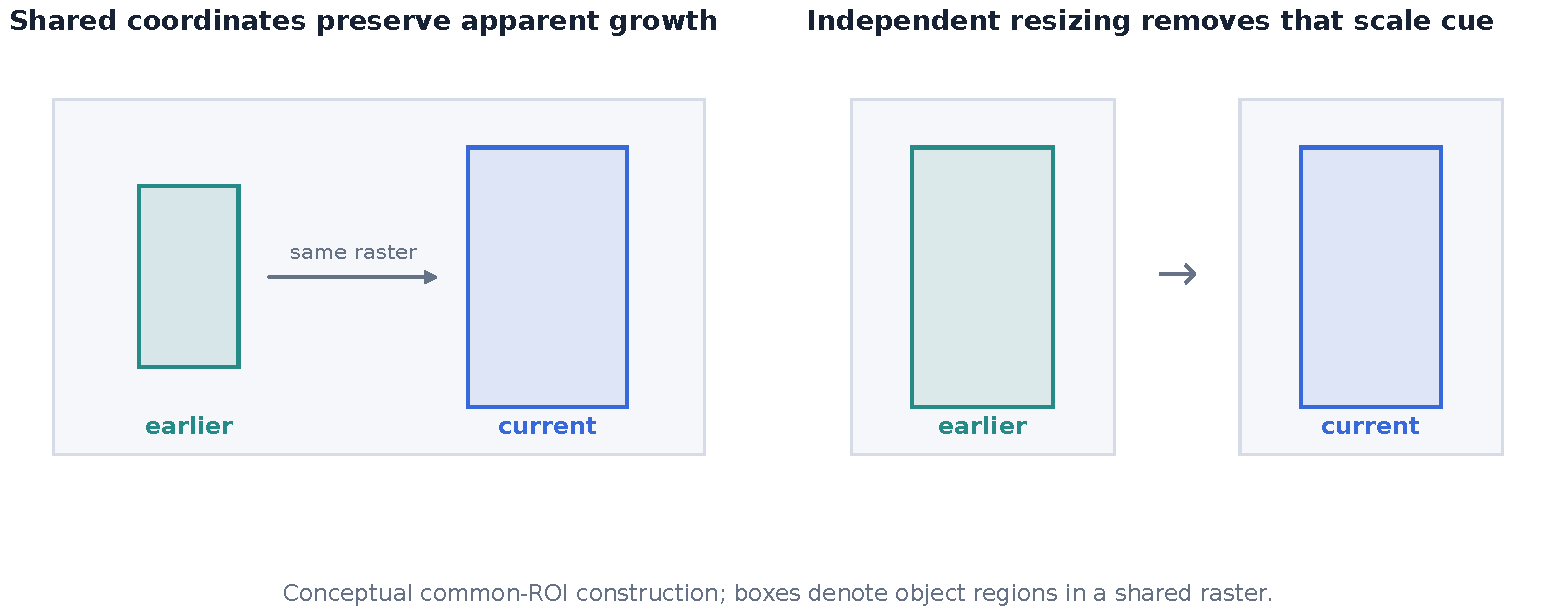
\includegraphics[width=\linewidth]{figures/crop_geometry.pdf}
\caption{\textbf{Shared coordinates preserve apparent expansion.} A common crop maps both endpoints at one spatial scale, whereas independent tight crops normalize away part of the size change. The diagram is schematic.}
\label{fig:crop}
\end{figure}

\begin{figure}[tbp]
\centering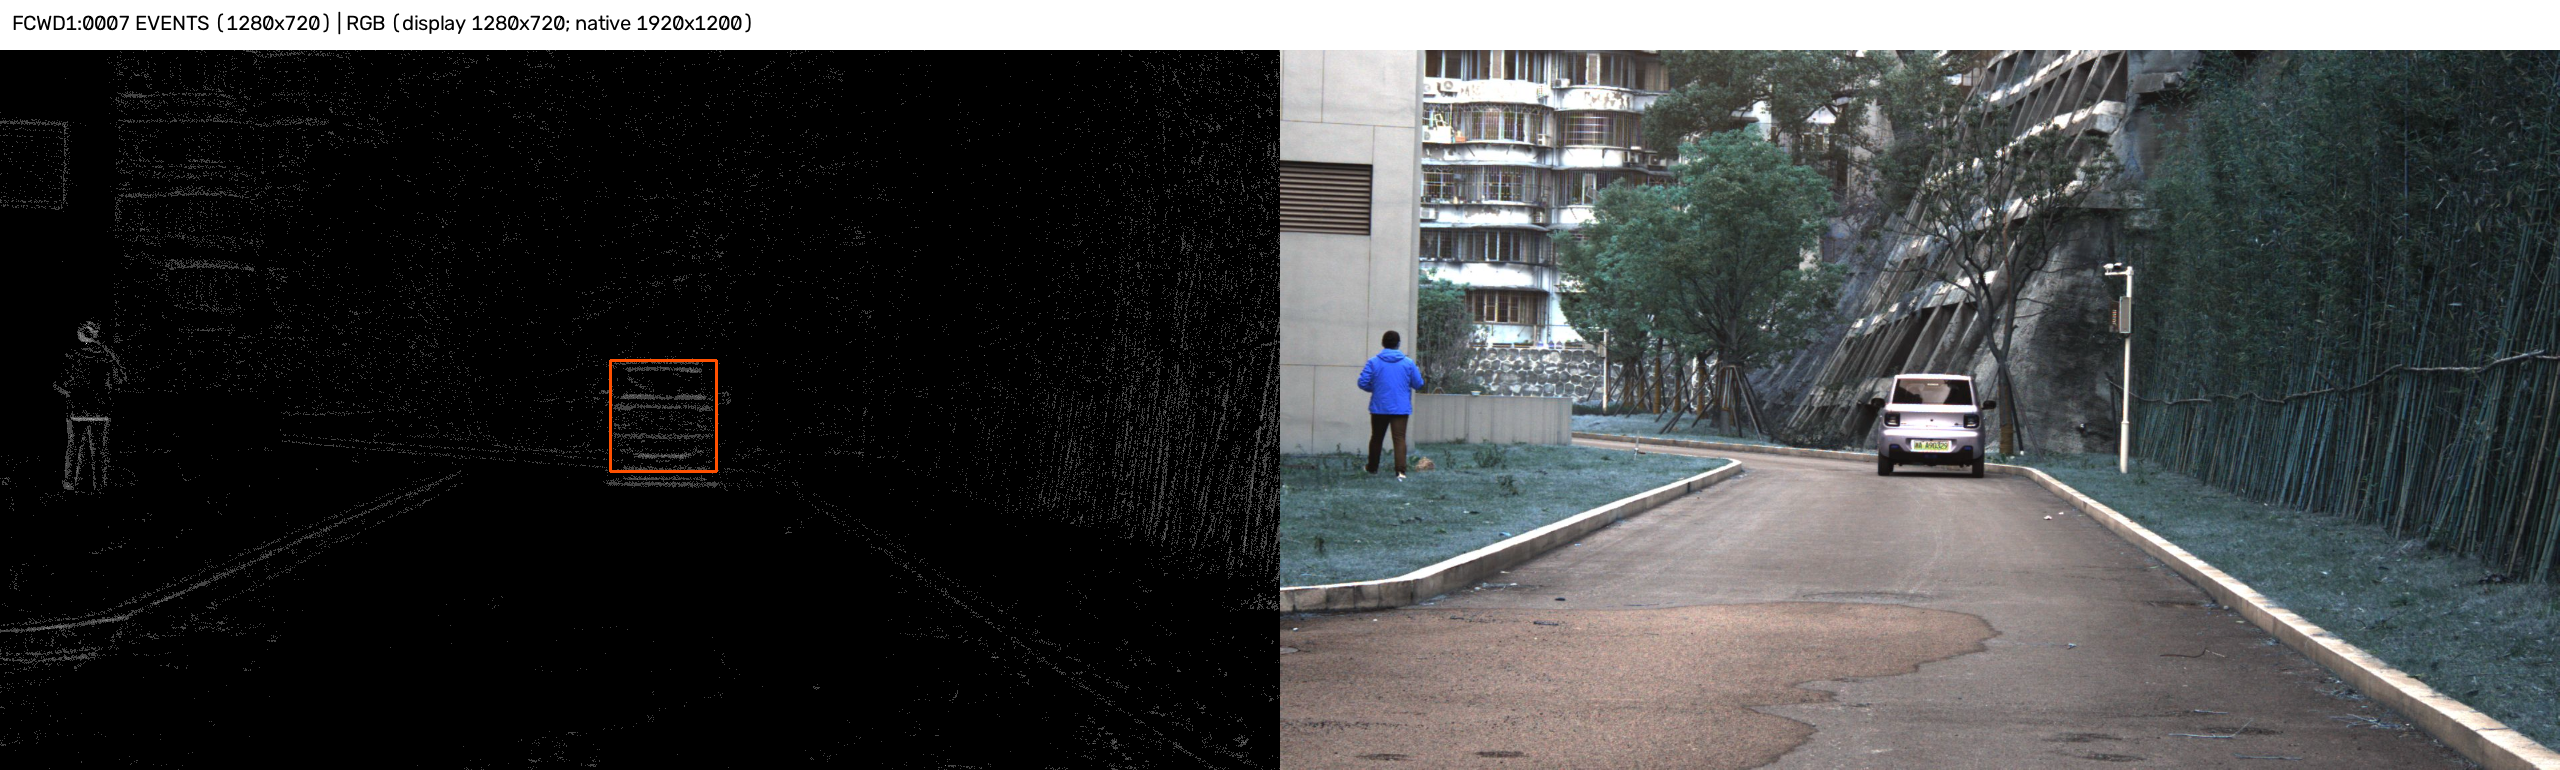
\includegraphics[width=\linewidth]{figures/fcwd_example.png}
\caption{\textbf{Event and RGB appearance for one object region.} FCWD1:0007 illustrates the cross-modal alignment problem. The orange region is the original visualization overlay.}
\label{fig:sensors}
\end{figure}

The eAP adapter reconstructs local targets from public three-dimensional tracks, whereas the benchmark uses private smoothed labels. Results therefore keep reconstructed eAP targets, EvTTC labels, and official GarlTTC labels in separate evaluation populations. \evidence{M01}

\subsection{Predictive embedding learning}
The generic JEPA implementation encodes a context representation with an online encoder $f_\theta$ and predicts a future latent conditioned on a horizon identifier:
\begin{equation}
 z_t=f_\theta(V_t),\qquad
 \widehat z_{t+h}=g_\psi(z_t,e_h),\qquad
 z_{t+h}^{\star}=\operatorname{sg}\bigl(f_\xi(V_{t+h})\bigr).
\end{equation}
The target starts from the online weights and is updated by an exponential moving average,
\begin{equation}
 \xi\leftarrow m\xi+(1-m)\theta.
\end{equation}
For multihorizon samples, a validity mask excludes unavailable future pairs from the alignment objective. The trainer supports normalized Smooth-L1 alignment, dense token prediction, spatial or tubelet masking, and variance or \texttt{visreg} regularization. Each experiment records its active loss configuration. \evidence{M04}

The V8 attribution experiment copies the \texttt{CausalScaleTTC} endpoint encoder and predicts three views of an unlabeled third endpoint from two earlier endpoints: dense features, a global geometry token, and foreground logits. Its objective is
\begin{equation}
 \mathcal L_{\mathrm{V8}}=\tfrac13\left(
 \mathcal L_{\cos}(\widehat D_2,D_2^\star)
 +\mathcal L_{\cos}(\widehat g_2,g_2^\star)
 +\mathcal L_{\mathrm{SL1}}(\widehat F_2,F_2^\star)\right).
\end{equation}
The scalar foreground-logit view uses Smooth-L1 because one-dimensional cosine similarity is almost everywhere constant. A frozen target encoder processes the future endpoint in evaluation mode under \texttt{no\_grad}. TTC, boxes, masks, category, metadata, geometry losses, contrastive losses, VICReg, and router outputs remain outside this objective. \evidence{M05}

V8 schedules EMA momentum by cosine interpolation between configured endpoints. It measures dispersion, effective rank, covariance trace, intersample similarity, and norm for the dense, global, and foreground views. A persistent-collapse rule aborts training when these diagnostics remain below their thresholds. Downstream probes then measure TTC utility.

V8 includes strict encoder transfer, random-frozen and scratch controls, partial-finetuning allowlists, and a shuffled-future control. The shuffled control uses a deterministic cross-track derangement that preserves the future marginal while holding the batch schedule, model, optimizer, update count, masking, augmentation, and EMA schedule fixed. Track identities construct the derangement and are excluded from model inputs. The declared gates require improvement over these controls before attributing a gain to predictive temporal structure. \evidence{M05}

\subsection{Spatial structure and temporal memory}
The high-resolution tubelet path preserves tokens as $[B,T,P,D]$, with distinct temporal and spatial patch axes. Images are padded on the right and bottom to a ceiling-based patch grid; invalid temporal positions and spatial padding carry masks. Windowed attention mixes spatial positions within a frame before a temporal mixer receives each patch trajectory. This separation prevents flattened raster order from being interpreted as time. \evidence{M06}

A block-causal Transformer permits attention among all spatial patches at the same instant and all earlier instants, while masking later frames. If token $i$ belongs to time $t_i$ and token $j$ to time $t_j$, its attention mask is $A_{ij}=\mathbf 1[t_j>t_i]$. A triangular token mask would impose an arbitrary left-to-right spatial ordering within each frame, so the implementation supplies the temporal block mask explicitly.

The recurrent delta-memory alternative maintains a separate matrix state per spatial patch and attention head. Writing the channelwise retention as $\alpha_t$, the implemented update is
\begin{align}
 \widetilde S_t&=\operatorname{diag}(\alpha_t)S_{t-1},\\
 e_t&=v_t-k_t^\top\widetilde S_t,\\
 S_t&=\widetilde S_t+\beta_t k_t e_t^\top,\qquad o_t=q_t^\top S_t.
\end{align}
Invalid patch steps retain the previous state and emit zero. State accumulation uses FP32, and the output returns to the input value dtype. Chunked execution passes explicit state between chunks and returns a detached final state, avoiding state shared between sequences. The causal recurrence uses no custom CUDA kernel. Tests establish equivalence between chunked and unchunked computation; runtime experiments determine deployment speed. \evidence{M06}

Before allocation, the implementation estimates quadratic attention-score memory,
$B H (TP)^2 b$ bytes for $H$ heads and $b$ bytes per value, and rejects layouts above the configured safety limit. Runtime evaluation reports observed memory, preprocessing time, and throughput.

\subsection{Causal scale, local transport, and TTC anchors}
The geometry-constrained model learns a foreground probability field and differentiable visible extent for each endpoint. It forms geometry tokens from the encoder token, log-height, centroid, foreground fraction, and sensor support. The analytic log-scale difference is supplemented by a bounded residual,
\begin{equation}
 r=\log h_2-\log h_1+\delta(a,b),\qquad
 \delta(a,b)=r_{\max}\tanh\!\left(\frac{u(a,b)-u(b,a)}2\right).
\end{equation}
With deterministic evaluation and reversed transport inputs, the residual changes sign under endpoint reversal. The primary output remains geometry-bound; the auxiliary direct inverse-TTC head does not feed into it. \evidence{M07}

The timestamp anchor matters. Under constant relative speed and apparent size inversely proportional to distance, the \emph{current-endpoint} inverse TTC is
\begin{equation}
 q_2=\frac{e^r-1}{\Delta t},\qquad T_2=\frac{\Delta t}{e^r-1}.
\label{eq:current-anchor}
\end{equation}
The learned-height-ratio reference implements
\begin{equation}
 T_1=\frac{\Delta t}{1-h_1/h_2}
     =\frac{\Delta t}{1-e^{-r}}=T_2+\Delta t,
\label{eq:start-anchor}
\end{equation}
which is anchored at the earlier endpoint under the same assumptions. Each route uses the convention determined by its label timestamp and evaluator. The benchmark phase defined below is a metric coordinate distinct from the current-endpoint log-scale difference. \evidence{M07,M10}

The transport extension derives event-native motion evidence from dense features $D_1,D_2$. It builds cosine correlations in a local neighbourhood $\mathcal N(p)$ and obtains expected displacement by
\begin{equation}
 P(\delta\mid p)=\frac{\exp\!\left(\langle\bar D_1(p),\bar D_2(p+\delta)\rangle/\tau\right)}
 {\sum_{\delta'\in\mathcal N(p)}\exp\!\left(\langle\bar D_1(p),\bar D_2(p+\delta')\rangle/\tau\right)},
 \quad d(p)=\sum_{\delta\in\mathcal N(p)}P(\delta\mid p)\delta.
\end{equation}
Out-of-bounds candidates are masked before softmax. The resulting summaries include translation, anisotropic and isotropic divergence, flow magnitude, confidence margin, entropy, and forward--reverse cycle error, with additional foreground-weighted variants. Coarse-to-fine models mix measurements from two scales through a learned gate. Shifted views replace a $[B,C,K,H,W]$ unfolded tensor to reduce intermediate memory. \evidence{M08}

Training-time RGB distillation introduces privileged visual supervision. The A4 DINOv3 teacher \citep{dinov3} supplies local cosine-similarity maps at six fixed feature-grid offsets. An L1 loss transfers these spatial relationships without requiring equal channel dimensions; slicing avoids circular wraparound. The student consumes events alone at inference, making this route privileged distillation rather than label-free self-supervision. \evidence{M09}

\subsection{Phase-domain routing and temporal refinement}
\label{sec:phase-refinement}
The later benchmark coordinate is
\begin{equation}
 \phi(T)=-\log\left(1-\frac{d}{T}\right),\qquad d=0.1\ \mathrm{s},
 \quad T<0\ \text{or}\ T>d.
\label{eq:benchmark-phase}
\end{equation}
Its inverse uses $q=-\operatorname{expm1}(-\phi)/d$. The implementation clamps phase to its configured support and saturates TTC magnitude at $60$ seconds; zero phase maps to $+60$ seconds. Saturation defines finite numerical output, while signed negative values represent recession. \evidence{M10}

\begin{figure}[H]
\centering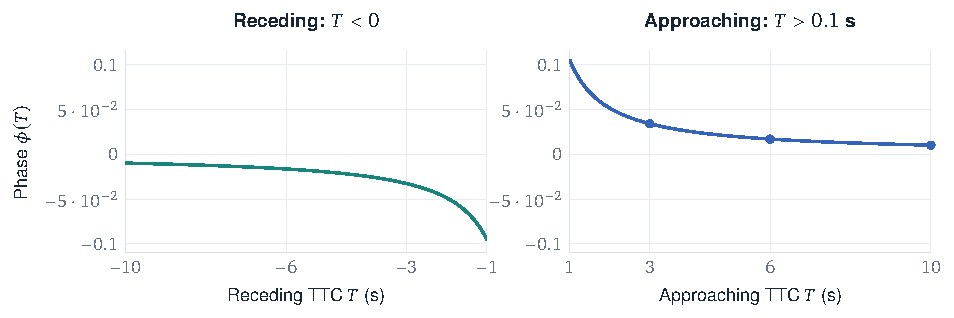
\includegraphics[width=\linewidth]{figures/rev_phase.pdf}
\caption{\textbf{Signed phase geometry.} Analytical curves show $|T|\in[1,10]$\,s on common vertical scales, with approaching-band markers at 3, 6, and 10\,s. The zoom excludes $[0,0.1]$\,s and the adjacent singularities.}
\label{fig:phase-geometry}
\end{figure}

The Simplex risk router selects among frozen expert TTCs by predicting relative expected absolute-phase costs. For three sorted expert phases, convexity and the 1-Lipschitz property of $\mathbb E|a-Y|$ imply ordered secant slopes $-1\leq s_0\leq s_1\leq1$. Softmax increments parameterize these constraints; integrating the slopes across expert-phase gaps yields relative costs. Hard selection returns one original expert prediction under a fixed tie order. The learned quantities are relative selection costs rather than calibrated collision probabilities. \evidence{M11}

The temporal refiner predicts a correction from a bounded feature history and four timing channels using a masked two-layer GRU; a causal Transformer provides the matched control. Histories require a contiguous valid suffix, and missing prefixes leave recurrent state unchanged. Residual mode anchors the phase at the median of the \emph{current} experts,
\begin{equation}
 \widehat\phi=\operatorname{median}(\phi_1,\phi_2,\phi_3)+0.03\,a_\theta(H).
\end{equation}
Separate heads predict phase-quantile widths and relative costs for the original experts; the latter do not estimate risk for the corrected output. Training combines phase absolute error, pinball losses, and relative-cost regression. Globally defined query mass supplies the weights without minibatch renormalization. Sparse-history variants retain selected slots from a longer history and recompute timing gaps from integer anchors, preserving cold starts and the original query population. \evidence{M12}

\subsection{Multimodal complement and uncertainty boundaries}
The later joint-measurement complement anchors on RGB phase and learns a correction from RGB features, event features, and the RGB phase itself:
\begin{equation}
 \widehat\phi=\phi_{\mathrm{RGB}}+s\,g_\theta
   ([z_{\mathrm{RGB}},z_{\mathrm{event}},\phi_{\mathrm{RGB}}]).
\end{equation}
The final layer starts at zero, so the initial prediction reproduces the RGB anchor up to native phase conversion. A matched ZERO control removes the complete event-feature block, including admitted event-clock features, while retaining network capacity. When RGB is absent, the model copies the event TTC without applying correction or averaging. The paired TRUE--ZERO comparison isolates the contribution of event information to the learned RGB correction. \evidence{M13}

Uncertainty has multiple meanings across these families. The causal-scale route predicts log-variance in log-ratio space and propagates it through the local Jacobian. For $q=\operatorname{expm1}(r)/\Delta t$,
\begin{equation}
 \operatorname{Var}(q)\approx \frac{e^{2r}}{\Delta t^2}\operatorname{Var}(r),\qquad
 \operatorname{Var}(T)\approx \frac{\Delta t^2e^{2r}}{(e^r-1)^4}\operatorname{Var}(r).
\end{equation}
The singularity near zero expansion requires separate finite-output and \texttt{known} indicators. The implementation marks unsupported or near-zero log-ratio predictions unknown and derives model-based threshold probabilities from an inverse-TTC Gaussian approximation. Empirical calibration requires measurements of coverage, calibration error, and corruption response. The temporal refiner's phase quantiles carry a different meaning from collision-class probabilities. \evidence{M07,M12}

\subsection{Optimization and execution semantics}
Component losses keep their true counts over each effective batch, and tail top-$k$ selection uses the complete effective batch instead of separate microbatches. Activation recomputation preserves random-number-generator state, keeping gradient accumulation and recomputation equivalent to the stated objective. The joint-measurement loss includes teacher relations, unlike the label-free JEPA loss. \evidence{M14}

Deployment optimizations include bounded event history, chunked memory, persistent input state, reusable feature caches, and graph execution. Because each changes state lifetime, numerical-parity tests accompany every admitted path. Runtime measurements state the associated preprocessing and inference boundary.
\section{Evaluation details and causal checks}
\label{app:evaluation-details}
This appendix describes data separation, causal checks, and runtime measurement in detail.

\subsection{The unit of independence}
Windows from one trajectory share appearance, geometry, object identity, and adjacent event history. We therefore partition complete sequence groups and resample at the sequence level. Small disjoint splits remain development evidence when the project has reused their sequences for diagnosis. \evidence{M16}

Recovery experiments keep every learned parent fold-local. Outer-development rows stay outside encoder fitting, teacher-derived caches, feature normalizers, and expert parents that feed the downstream model. A frozen parent still carries its prior exposure, so the analysis follows sample membership through preprocessing, checkpoints, cached features, normalization, and model selection.

A deterministic event representation can be reused when preprocessing and sample identity stay fixed. A checkpoint fitted on a larger population changes the exposure of every downstream result. File identity verifies which representation or model was used; training membership determines the strength of the resulting claim. \evidence{M17}

\subsection{Paired inference at the sequence level}
Comparisons pair the same eligible rows and sequences. For per-row metric differences $d_{si}$ in sequence $s$, the sample-weighted estimate is
\begin{equation}
 \widehat\Delta=\frac{\sum_s\sum_{i=1}^{n_s}d_{si}}{\sum_s n_s}.
\end{equation}
A paired sequence bootstrap samples sequence identities with replacement and carries every row from each selected sequence into the replicate. Sample-weighted resampling recomputes the ratio of summed differences to summed counts; the sequence-macro calculation averages sequence means. The scorer-based comparison uses the sample-weighted form with a fixed bootstrap seed, complete sequence clusters, and no removal of invalid MiD rows. \evidence{M15}

Intervals based on few sequences have limited precision and inherit development exposure and experiment multiplicity. Random seeds measure optimization variation for a fixed split, whereas out-of-fold partitions vary the held-out groups. Results report seeds, folds, and sequences separately.

\subsection{Causality tests}
Prefix-invariance tests determine whether later inputs alter an earlier output. The causal-scale suite checks foreground logits, geometry tokens, pair tokens, analytic and residual log-ratios, and TTC. A legacy symmetric smoother provides a positive control by violating prefix invariance; the causal-left mode must remain invariant under the same perturbation. \evidence{M18}

Network masks alone cannot establish causality. Tests also perturb crop coordinates, normalization inputs, teacher frames, and labels. Self-supervised samples must remain unchanged when labels change, and crop tests restrict geometry to the designated endpoint boxes. \evidence{M03,M18}

Streaming tests cover state reset and update semantics. The bounded object-ROI estimator rejects timestamp rollback until reset, validates aligned packets and coordinates, and discards events outside its history. It consumes ROI-local event coordinates and supplied object observations. Paced replay then adds acquisition, queuing, temporal state, multiple objects, and host-visible output. \evidence{M19}

\subsection{Matched controls and the scope of attribution}
Architectural ablations match rows, seeds, training budgets, parent exposure, selection rules, and model capacity. A zeroed-input model removes modality information while retaining capacity. A shuffled-future control disrupts temporal correspondence while preserving the future marginal and optimization schedule. A frozen random encoder measures what the downstream head can recover without learned features.

A hard router selects among fixed expert predictions; a residual phase model can correct them. Teacher distillation measures the effect of privileged RGB supervision on an event backbone. Failed and vetoed arms remain in the analysis because they constrain mechanism-level explanations.

\subsection{Latency, memory, and sustained service}
A tensor-forward benchmark starts after tensor preparation. The paced runner instead includes a RAW producer, absolute arrivals, a bounded queue, and host-visible output. Completion occurs when the consumer returns every required prediction. Fixed arrivals expose backlog, while the results record drops, acquisition errors, incomplete histories, and invalid outputs. \evidence{M20}

The primary deadline-to-output response is
\begin{equation}
 L_i=t_i^{\mathrm{host\ output}}-t_i^{\mathrm{scheduled\ arrival}}.
\end{equation}
A secondary clock starts after RAW acquisition. Deadline evaluation reports tail quantiles, maximum response, coverage, backlog, and drops because mean response can hide missed arrivals. Warmup uses data available before the first admitted anchor. The 50-Hz milestone requires sustained cadence, numerical parity, and complete finite outputs. \evidence{M20}

The available RAW sequences are shorter than the sustained-service milestone. The replay therefore characterizes short-run latency for its hardware, population, numerical tolerance, and duration.

Implementation checks and their scope are reported in Appendix~\ref{app:reproduction}. \evidence{M21} The official leaderboard score evaluates prediction accuracy; it provides no measurement of sensor-to-output latency or sustained service.
\clearpage
\section{Paired transfer uncertainty and numerical cases}
\label{app:derived-transfer}
We analyze the saved query-level predictions in \path{data/transfer_queries.csv} (L46). Source key R01 maps the derived results to \path{revision/derived_transfer_analysis.json}; \path{scripts/prepare_revision.py} regenerates them.

\subsection{Exact paired sequence bootstrap}
The analysis uses the 468 eligible Extended-new predictions and their 32 physical-sequence groups. Each of 10,000 replicates samples 32 group identities with replacement and includes every query from each sampled group. Repeated groups contribute repeated queries. PHASE-TTC and RGB share the sampled indices. For each model, we compute pooled mean, median, and 95th-percentile absolute error, then form the PHASE-minus-RGB difference. NumPy's \texttt{linear} quantile convention and \texttt{default\_rng(20261028)} define the 2.5th and 97.5th percentile endpoints.

The point differences are \RevisionMeanDelta\,s for the mean, \RevisionMedianDelta\,s for the median, and \RevisionPninetyfiveDelta\,s for p95. All three intervals contain zero (Table~\ref{tab:revision-bootstrap}). The exploratory intervals condition on the fitted models and development-exposed sequences; they do not incorporate representation-training variability or adaptive model selection.

Differences use full-precision predictions. The mean difference rounds to $+0.007$\,s; subtracting the separately rounded means 1.023 and 1.015 instead gives $+0.008$\,s.

\subsection{Numerical cases}
The two queries below maximize and minimize the PHASE-minus-RGB absolute-error difference within the saved predictions. These post hoc examples show the range of model disagreement; their causes would require inspection of the corresponding sensor observations.
\begin{table}[H]\centering\small
\caption{Queries with the largest positive and negative PHASE-minus-RGB absolute-error differences in the labeled transfer set. \evidence{R01,L46}}
\label{tab:revision-cases}
\begin{tabularx}{\linewidth}{@{}Xrrrr@{}}\toprule
Query & Target (s) & PHASE (s) & RGB (s) & $\Delta$ AE (s)\\\midrule
{\footnotesize\path{CPNAO-high:13700430}} & 2.996 & 6.604 & -12.903 & -12.290\\
{\footnotesize\path{CCRs-1-medium-100-overlap-100:5950352}} & 6.765 & -25.740 & -9.880 & +15.861\\
\bottomrule\end{tabularx}\end{table}
\FloatBarrier

\clearpage
\subsection{Complete sequence comparisons}
\begin{figure}[H]
\centering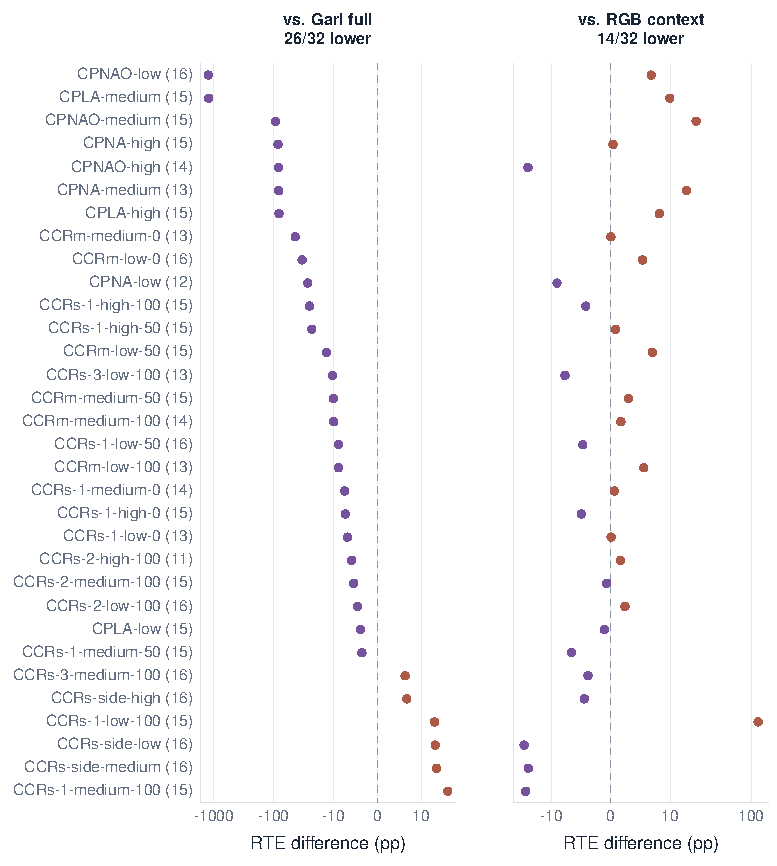
\includegraphics[width=\linewidth,height=.70\textheight,keepaspectratio]{figures/rev_sequence.pdf}
\caption{\textbf{Sequence-level relative TTC error differences.} Both panels show the 32 labeled Extended-new sequences in a common order; parentheses give query counts and negative values favor PHASE-TTC. The symmetric-log axes are linear between $-5$ and $+5$ percentage points. Display labels omit repeated overlap suffixes; Table~\ref{tab:sequence-full} gives the full identities. \evidence{R01,L46}}
\label{fig:transfer-sequence}
\end{figure}
\FloatBarrier
\clearpage
{\small\begin{longtable}{@{}p{6.0cm}rrrrr@{}}
\caption{Query counts and mean RTE (\%) for all 32 Extended-new sequences. Differences are in percentage points. \evidence{R01,L46}}\label{tab:sequence-full}\\
\toprule Sequence & $n$ & PHASE & RGB & Garl & $\Delta_{\rm RGB}$\\\midrule\endfirsthead
\toprule Sequence & $n$ & PHASE & RGB & Garl & $\Delta_{\rm RGB}$\\\midrule\endhead
\bottomrule\endfoot
CPNAO-low & 16 & 46.95 & 41.09 & 1283.26 & +5.86\\
CPLA-medium & 15 & 45.43 & 35.53 & 1265.98 & +9.90\\
CPNAO-medium & 15 & 41.92 & 20.94 & 134.36 & +20.98\\
CPNA-high & 15 & 66.50 & 66.14 & 150.71 & +0.36\\
CPNAO-high & 14 & 55.86 & 75.18 & 137.89 & -19.31\\
CPNA-medium & 13 & 59.61 & 43.68 & 141.20 & +15.93\\
CPLA-high & 15 & 62.29 & 54.92 & 143.22 & +7.37\\
CCRm-medium-0-overlap-0 & 13 & 14.61 & 14.57 & 57.78 & +0.04\\
CCRm-low-0-overlap-0 & 16 & 16.40 & 11.85 & 49.69 & +4.56\\
CPNA-low & 12 & 35.90 & 44.34 & 62.54 & -8.44\\
CCRs-1-high-100-overlap-100 & 15 & 19.23 & 22.75 & 44.19 & -3.52\\
CCRs-1-high-50-overlap-50 & 15 & 18.25 & 17.55 & 41.09 & +0.71\\
CCRm-low-50-overlap-50 & 15 & 17.70 & 11.67 & 30.65 & +6.02\\
CCRs-3-low-100-overlap-100 & 13 & 8.35 & 15.08 & 18.67 & -6.73\\
CCRm-medium-50-overlap-50 & 15 & 20.93 & 18.41 & 30.93 & +2.53\\
CCRm-medium-100-overlap-100 & 14 & 15.25 & 13.79 & 25.04 & +1.47\\
CCRs-1-low-50-overlap-50 & 16 & 4.98 & 8.93 & 13.15 & -3.95\\
CCRm-low-100-overlap-100 & 13 & 20.69 & 15.96 & 28.85 & +4.73\\
CCRs-1-medium-0-overlap-0 & 14 & 6.72 & 6.17 & 13.14 & +0.55\\
CCRs-1-high-0-overlap-0 & 15 & 17.32 & 21.49 & 23.61 & -4.17\\
CCRs-1-low-0-overlap-0 & 13 & 9.81 & 9.73 & 15.58 & +0.07\\
CCRs-2-high-100-overlap-100 & 11 & 13.75 & 12.35 & 18.65 & +1.40\\
CCRs-2-medium-100-overlap-100 & 15 & 6.84 & 7.39 & 11.36 & -0.55\\
CCRs-2-low-100-overlap-100 & 16 & 15.67 & 13.62 & 19.44 & +2.05\\
CPLA-low & 15 & 25.19 & 26.09 & 28.38 & -0.90\\
CCRs-1-medium-50-overlap-50 & 15 & 5.73 & 11.32 & 8.66 & -5.60\\
CCRs-3-medium-100-overlap-100 & 16 & 15.32 & 18.54 & 9.91 & -3.21\\
CCRs-side-high & 16 & 21.54 & 25.26 & 15.77 & -3.72\\
CCRs-1-low-100-overlap-100 & 15 & 395.63 & 273.53 & 378.78 & +122.10\\
CCRs-side-low & 16 & 41.76 & 63.28 & 24.48 & -21.52\\
CCRs-side-medium & 16 & 46.06 & 65.11 & 27.92 & -19.05\\
CCRs-1-medium-100-overlap-100 & 15 & 111.28 & 131.87 & 83.19 & -20.60\\
\end{longtable}}
\section{Competition adaptation and complete prediction traces}
\label{app:competition-details}
This appendix details input construction and timing for the 434-query competition population. Linear and symmetric-log views show the full signed prediction traces.

\subsection{Frozen models and causal input construction}

We use the public Hugging Face full, event-only, and visual-only checkpoints with their released configurations and source revision. Strict state-dictionary loading and float32 inference keep each model fixed. The release identifies the checkpoint bytes but does not document complete training membership, so the evaluation represents frozen-checkpoint adaptation rather than a claim of clean zero-shot transfer.

Garl-TTC predicts the ratio of object heights at two endpoints and converts it to TTC as
\begin{equation}
 \widehat T
 =\frac{\Delta t_{\mathrm{measured}}}
 {1-\widehat h_0/\widehat h_1}.
 \label{eq:garl-height-ratio-evttc}
\end{equation}
The released configuration sets the native model field $\mathrm{dT}=0.1$\,s. For Equation~\ref{eq:garl-height-ratio-evttc}, the adapter substitutes the measured separation of each endpoint pair while leaving the released representation unchanged. The checkpoint metadata do not establish the cadence used during training.

The full and visual routes select the latest real RGB frame at or before a query, then the preceding frame closest to 100\,ms earlier. Full Garl builds one causal event window per RGB endpoint with support capped at $\min(\Delta t_{\mathrm{measured}},100\,\mathrm{ms})$. Event-only Garl uses two consecutive 100\,ms windows after startup and splits the observed causal prefix into two intervals for earlier queries. Each endpoint uses the released 20-plane, polarity-agnostic time volume. Queries without sufficient history remain gaps.

PHASE-TTC uses its declared 650\,ms causal history. The shared query population therefore compares the frozen systems under their respective temporal support.

Supplied boxes use zero-based, half-open event-plane coordinates. The adapter selects the latest box available at each endpoint; if the endpoint precedes all query-causal boxes, it uses the earliest such box and records availability at query time. Road sequences pair right Blackfly RGB with right Prophesee events. Slider uses its supplied streams and a rotation derived from camera poses because its calibration lacks a named event-to-RGB extrinsic. Calibrated intrinsics, distortion, and rotation-only ray projection map the event box into RGB; unavailable object depth precludes translational correction. A common square edge spans the endpoint boxes, with endpoint-specific event centers and the current center applied to both RGB frames.


\subsection{Published three-sequence comparison}
Table~VI of the eAP paper reports Garl-TTC on three EvTTC sequences, with an unweighted mean RTE of 10.60\% \citep{eap}. That study uses a separate labeled population; shared scenario names do not establish shared recordings or query identities. \evidence{T02}
\begin{table}[H]
\centering\small
\caption{Garl-TTC's published zero-shot relative TTC error on three EvTTC sequences, as reported in the eAP paper, Table VI. \evidence{T02}}
\label{tab:evttc-published-rte}
\begin{tabular}{@{}lr@{}}
\toprule
\textbf{Published sequence} & \textbf{RTE (\%)} \\
\midrule
CCRs2-medium & 8.31 \\
CCRs2-high & 10.56 \\
CCRm-medium & 12.93 \\
\textbf{Unweighted average} & \textbf{10.60} \\
\bottomrule
\end{tabular}
\end{table}
\begin{table}[H]
\centering\scriptsize
\caption{Garl--PHASE prediction comparisons for all ten sequences. Each entry gives shared-finite coverage and median absolute prediction difference in seconds. \evidence{T01}}
\label{tab:evttc-sequence-disagreement}
\setlength{\tabcolsep}{3.2pt}
\begin{tabular}{@{}lrrr@{}}
\toprule
\textbf{Sequence} & \textbf{Full $n/N$; med.} & \textbf{Event $n/N$; med.} & \textbf{Visual $n/N$; med.} \\
\midrule
CCRs1-low & 49/50; 0.465 & 50/50; 0.776 & 49/50; 0.213 \\
CCRs1-medium & 42/43; 0.308 & 43/43; 0.863 & 42/43; 0.200 \\
CCRs1-high & 29/30; 0.207 & 30/30; 0.519 & 29/30; 0.111 \\
CCRs2-low & 45/46; 0.221 & 46/46; 0.339 & 45/46; 0.243 \\
CCRs2-medium & 54/55; 0.178 & 55/55; 1.045 & 54/55; 0.254 \\
CCRs2-high & 58/59; 0.188 & 59/59; 0.682 & 58/59; 0.223 \\
CCRm-low & 41/42; 0.270 & 42/42; 0.703 & 41/42; 0.283 \\
CCRm-medium & 39/40; 0.151 & 40/40; 0.839 & 39/40; 0.350 \\
Slider-750 & 49/51; 0.408 & 51/51; 0.470 & 51/51; 0.258 \\
Slider-1000 & 18/18; 0.288 & 18/18; 0.119 & 18/18; 0.067 \\
\bottomrule
\end{tabular}
\end{table}

\subsection{Runtime boundary and interpretation}

\begin{table}[H]
\centering\small
\caption{Offline processing time in seconds per query. Model time covers the synchronized forward pass and host output; full time includes tensor preparation. The Garl variants ran in full/event/visual order; PHASE-TTC used its own adapter and history length. \evidence{T01}}
\label{tab:evttc-runtime}
\begin{tabular}{@{}lrrrr@{}}
\toprule
\textbf{Model} & \textbf{Model med.} & \textbf{Model P95} & \textbf{Full med.} & \textbf{Full P95} \\
\midrule
PHASE-TTC & 0.753 & 7.820 & 2.687 & 9.073 \\
Garl full & 0.039 & 0.045 & 0.542 & 1.009 \\
Garl event-only & 0.007 & 0.011 & 0.350 & 0.806 \\
Garl visual-only & 0.007 & 0.011 & 0.158 & 0.221 \\
\bottomrule
\end{tabular}
\end{table}

Timing separates tensor preparation from the synchronized model-to-host call and excludes loading, indexing, calibration, source hashing, and result serialization. The variants run once in full, event-only, visual-only order, so operating-system and HDF5 caches and GPU warm state can carry between runs. Table~\ref{tab:evttc-runtime} reports these observations alongside PHASE-TTC, whose adapter and temporal support differ.

Independent verification accounts for each planned record and replays the float32 height-to-TTC conversion. Full and visual Garl remain partial because of input gaps; event-only contains all 434 rows. Across the ten sequences, the four routes exhibit distinct signed behavior and disagreement tails. \evidence{T01}

\clearpage
\subsection{All ten sequences, with missing inputs preserved}
\begin{figure}[H]
\centering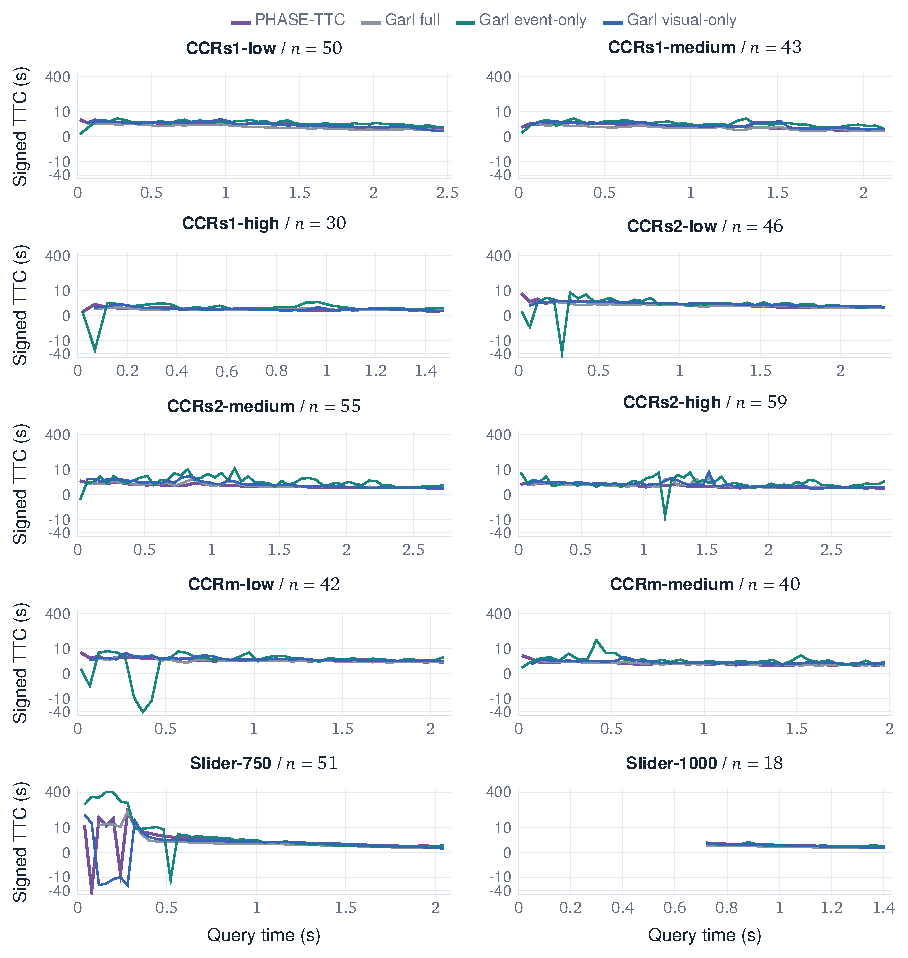
\includegraphics[width=\linewidth,height=.72\textheight,keepaspectratio]{figures/rev_competition_symlog.pdf}
\caption{\textbf{Signed predictions on a symmetric-log scale.} PHASE-TTC is purple, Garl full gray, event-only teal, and visual-only blue. All panels are linear inside $[-2,2]$\,s and logarithmic outside; gaps mark unavailable inputs. \evidence{T01}}
\label{fig:evttc-predictions-symlog}
\end{figure}
\clearpage
\begin{figure}[H]
\centering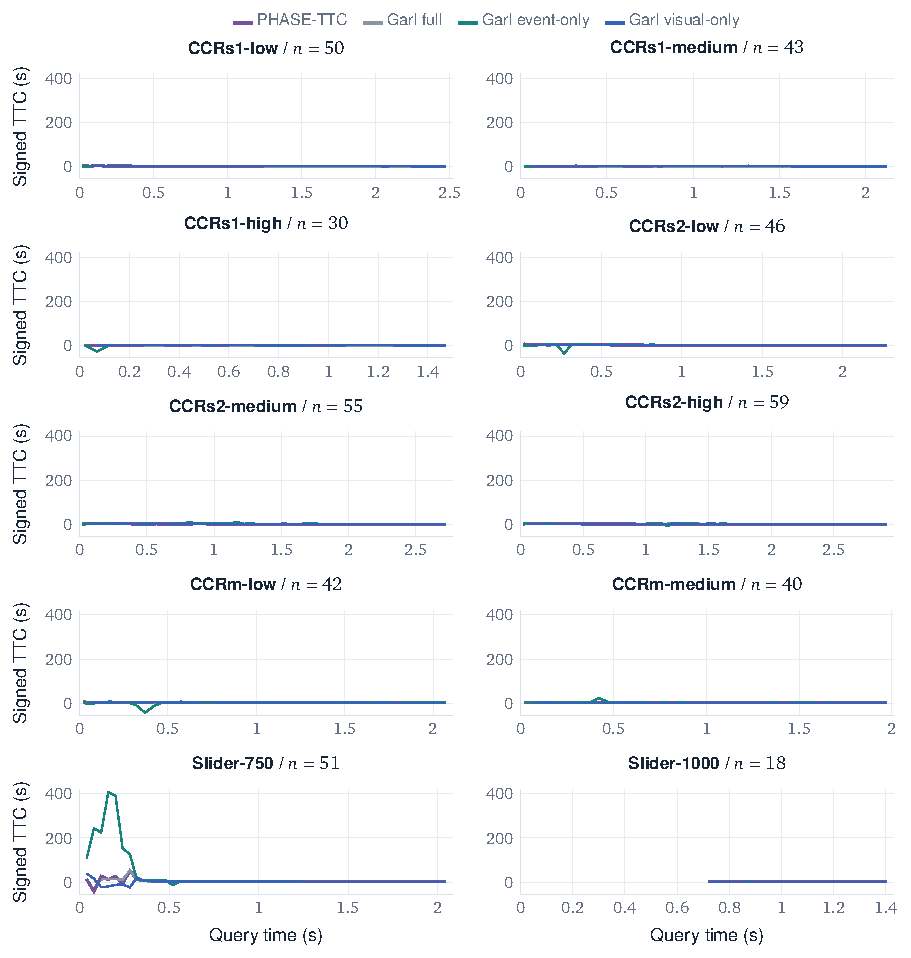
\includegraphics[width=\linewidth,height=.72\textheight,keepaspectratio]{figures/rev_competition_linear.pdf}
\caption{\textbf{Signed predictions on a common linear scale.} The same outputs as Figure~\ref{fig:evttc-predictions-symlog} show the full excursion range, which compresses the central values. \evidence{T01}}
\label{fig:evttc-predictions-linear}
\end{figure}
\FloatBarrier

\clearpage
\section{The initial representation-learning programme}
\label{sec:early}

PHASE-TTC began as E-JEPA-TTC, a study of predictive event representations for time-to-contact estimation. The programme covered pooled and spatial embeddings, apparent expansion, and transport-conditioned residual dynamics. Some models improved TTC while losing the geometric behaviour that motivated them, so the experiments assessed accuracy, geometric consistency, and representation content separately.

The historical names distinguish otherwise similar version numbers. \emph{Causal Scale v5--v8} refers to synthetic operator tests, whereas \emph{Scientific Recovery V5--V8} refers to later real-data studies. The EvTTC and eAP A0/A1 experiments also used different data and metrics.

\begin{figure}[htbp]\centering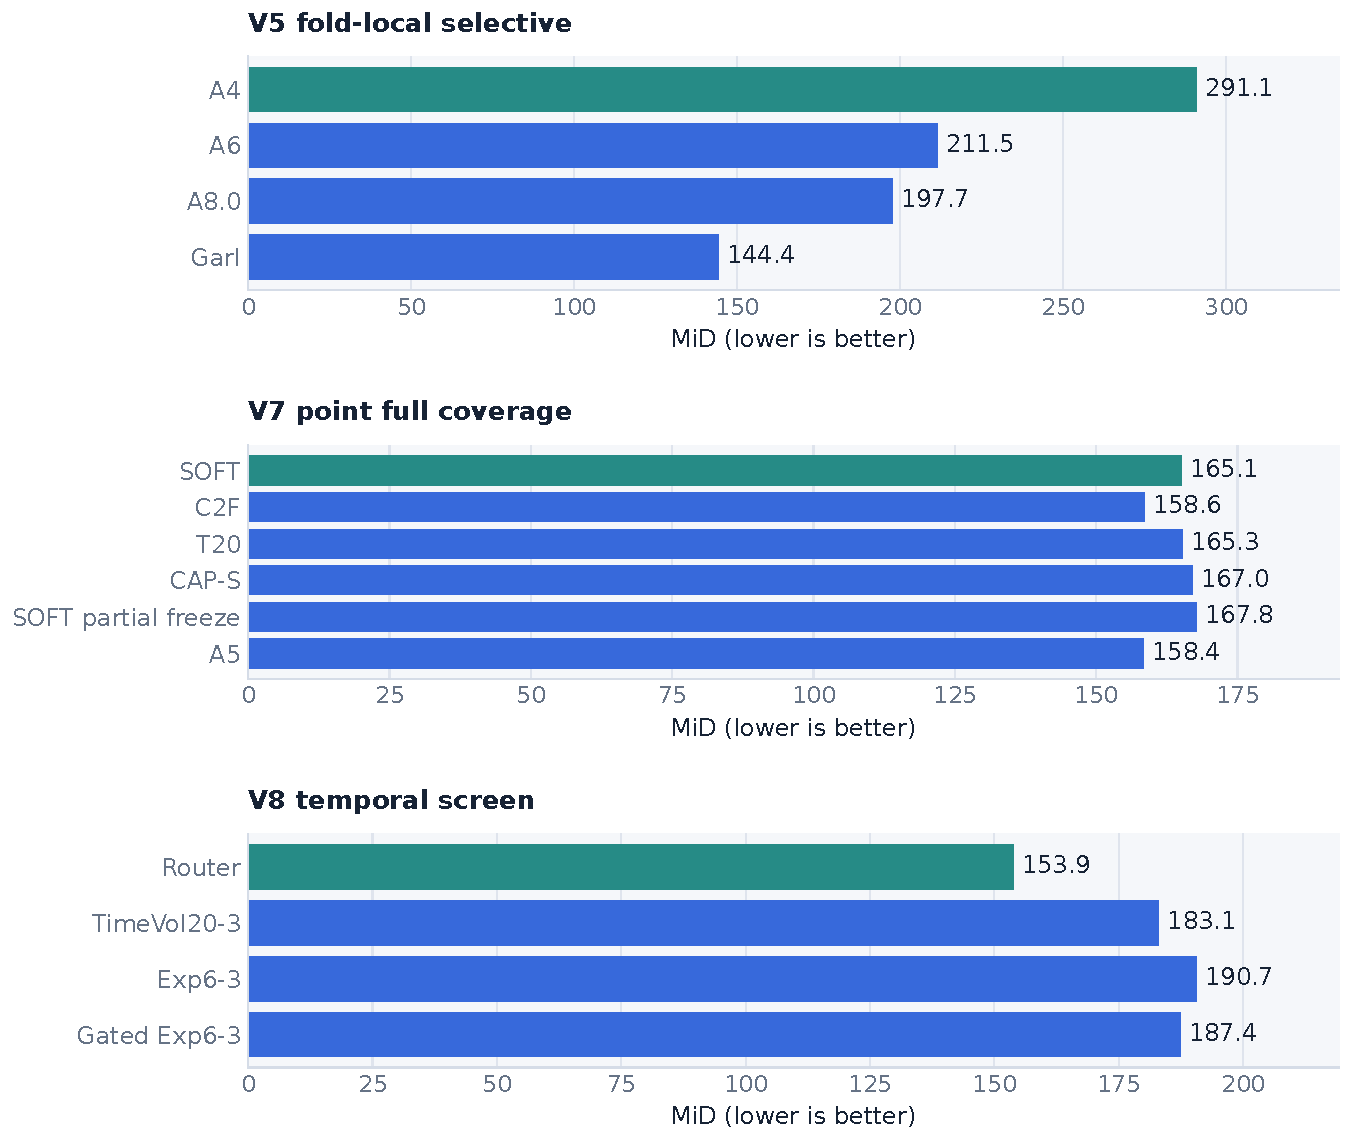
\includegraphics[width=\linewidth]{figures/early_ablation.pdf}
\caption{Early recovery results by experiment family; lower MiD is better.}\label{fig:early}
\end{figure}

\subsection{Global and dense representations on EvTTC}

Global A0 remained preferable to Dense A1 in the matched EvTTC comparison. Five grouped folds and seeds 7, 13, and 21 produced fifteen paired runs per model (Table~\ref{tab:early-evttc}). \evidence{E01}

\begin{table}[htbp]
\centering\small
\begin{tabular}{lrrr}
\toprule
Architecture & MAE (s) & Relative error (\%) & Selection score \\
\midrule
Global A0 & 1.0109 & 30.25 & 0.58452 \\
Dense A1 & 1.0067 & 30.55 & 0.59312 \\
\bottomrule
\end{tabular}
\caption{Global A0 and Dense A1 means over five EvTTC folds and three seeds.}
\label{tab:early-evttc}
\end{table}

Dense A1 reduced mean absolute error, but increased both relative error and the registered composite selection score. It also used 2.16 times A0's measured latency and 1.58 times its training time. We retained the smaller global model. \evidence{E01}

Attention residuals, temporal KDA/Object-KDA, object-conditioned crops, and FlowMimic-style alignment all failed their selection gates. Because those screens used different data or criteria, they do not extend the matched A0/A1 ranking.

\subsection{Representation variance and dynamic information}

The temporal-residual objective captured the desired dynamics under a slow synthetic nuisance process. Its mean dynamic $R^2$ was about $0.72$, versus $0.15$ for variance regularization. The latter maintained high embedding variance while preserving nuisance information, showing that variance alone was a poor proxy for useful temporal content. \evidence{E02}

Changing the nuisance on every frame reversed the result: the residual objective's dynamic $R^2$ became negative, while the variance control reached about $0.74$. Later probes kept both level and change features and varied the nuisance process. Neither effective rank nor per-dimension standard deviation demonstrated TTC-relevant content on its own. \evidence{E02,E12}

\subsection{Object identity and crop geometry}

Object-level eAP/GarlTTC requires an explicit query because several annotated objects can share one event frame while having different TTC values. Object-LHR resolved the ambiguity by cropping the selected object at both endpoints before estimating temporal scale.

Independent resizing erased much of the apparent scale change required by the geometric head. Object-Expansion v2 stabilized the output by predicting sign and log inverse-TTC magnitude; Object-Signed-Expansion v3 combined them in one expansion coordinate and added ordered temporal features plus box motion. Perturbation tests showed strong dependence on box motion and little response to events, so this accuracy could not be credited to event representation learning.

Object Event v4 placed three causal endpoints in one common crop, preserving apparent growth and separating the neural event path from the motion ablation. The object query and its coordinate system became part of the model specification. Earlier variants used different conditions and remain separate experiments.

\subsection{Physical tests of the scale operator}

The frozen v4.31 matcher passed representation-stability checks but failed the zoom, reversal, and translation requirements. We also found uncommitted source changes and a missing evidence stage, so the run was ineligible for selection. Its foreground, height, pseudoflow, and correspondence diagnostics motivated a new scale estimator.

For two apparent heights $h_{t-1}$ and $h_t$ separated by $\Delta t$, the Causal Scale operator defines
\begin{equation}
 r_t=\log h_t-\log h_{t-1},\qquad
 \widehat{\tau_t^{-1}}=\frac{\exp(r_t)-1}{\Delta t}.
 \label{eq:early-scale}
\end{equation}
Under idealised constant-speed approach, this gives inverse TTC at the newer endpoint. Changes in shape, viewpoint, occlusion, or relative motion can violate the geometric assumptions. For $\hat\tau_t=\Delta t/(\exp(r_t)-1)$, the sensitivity is
\begin{equation}
 \frac{\partial\hat\tau_t}{\partial r_t}
 =-\frac{\Delta t\exp(r_t)}{(\exp(r_t)-1)^2}.
\end{equation}
The derivative grows without bound as $r_t$ approaches zero. Output clipping can contain the resulting TTC value, but it cannot improve the scale measurement.

The learned foreground failed to reproduce the ideal operator on held-out synthetic data. Causal Scale v5 reached correlation $0.92$ with translation leakage $0.027$, missing both requirements. V7 reduced leakage to $0.0034$ and symmetric TTC error to $0.25$, but correlation stayed at $0.92$ and the validation result did not transfer to the new synthetic group. \evidence{E13,E14}

Causal Scale v8 selected on both mean and worst-group performance across independent synthetic groups. Fixed symmetric smoothing supported sparse endpoints, and a final CVaR loss emphasized large ratio errors. Correlation remained below the gate in every group. We nevertheless continued to a real-data screen, treating it as exploratory. \evidence{E15}

\subsection{Foreground supervision in the first eAP screens}

The first eAP screens used a common object crop, three event endpoints, and oracle boxes; they did not evaluate detection. A0 learned a weak rectangular foreground target. A1 replaced it with height, width, and centre supervision. A1-FR added a full-resolution decoder, A1-DF used deeper features, and A1-DF-R supervised the pair ratio directly. A3 kept the A1 architecture and trained with RGB-derived SAM masks. All screens reused public validation data.

\begin{table}[htbp]
\centering\small
\begin{tabular}{lrr}
\toprule
Arm & MiD $\downarrow$ & Failure (\%) \\
\midrule
A1 geometry & 346.829 & 9.961 \\
A3 SAM distilled & 353.635 & 10.889 \\
Garl trained matched & 203.634 & 0.000 \\
\bottomrule
\end{tabular}
\caption{Early eAP public-validation results for A0, A1, A3, and matched Garl.}
\label{tab:early-screen}
\end{table}

A3 did not improve on A1, and both scored worse in aggregate MiD than matched Garl. The diagnostics showed that estimating absolute height did not guarantee recovery of its temporal derivative. Garl achieved lower aggregate error but predicted positive TTC for receding cases, leaving signed motion unresolved. \evidence{E25,E26}

A4 distilled local spatial relations from a frozen DINOv3 RGB teacher into an event student; A4D also learned changes in those relations across endpoints. Both used RGB during training and events at inference. A5 and A6 then varied TTC specialization and transport while monitoring the inherited geometry.

\subsection{Scientific Recovery V5: fold-specific producer training}

The first grouped-development run inherited an A4 parent trained on all nine development sequences, including each held-out outer group. We excluded it from promotion and retrained A4 inside every outer fold. The corrected study initialized A6 and A8.0 from the matching fold-local parent and trained Garl from scratch. \evidence{E03}

The comparison matched samples, targets, training budget, metric, and oracle-ROI access. The E-JEPA-family branch used three endpoints and twelve channels; Garl used two endpoints and forty channels. Checkpoint selection still used the outer-development split, and TTC buckets shaped the initial 8,192-token sample. Thus, the correction removed parent exposure without turning the study into a blind test or a target-free sample. \evidence{E03}

\begin{table}[htbp]
\centering\small
\begin{tabular}{lrrr}
\toprule
Model & Parameters & MiD $\downarrow$ & Failure (\%) \\
\midrule
A4 parent & 355,118 & 291.088 & 9.448 \\
A6 transport & 498,130 & 211.509 & 7.849 \\
A8.0 dual transport & 627,827 & 197.691 & 7.019 \\
V6.1 radius 2 & 627,827 & 194.122 & 6.689 \\
A5 causal & 424,274 & 155.472 & 4.761 \\
Garl local matched & 24,674,178 & 144.353 & 0.000 \\
\bottomrule
\end{tabular}
\caption{Scientific Recovery V5--V6 results on 8,192 tokens from nine sequences, three folds, and seed 7.}
\label{tab:early-v5v6}
\end{table}

A8.0, which freed transport while retaining the frozen parent geometry, improved MiD over A6 by 13.8 points; the paired 95\% interval was $[-17.7,-10.1]$. It still exceeded the preregistered MiD threshold of 175 and remained behind Garl, so V5 produced no candidate. \evidence{E03,E05}

Sequence-scoped track identifiers and preserved token/target IDs made the fold-local correction auditable through the full training lineage.

\subsection{Scientific Recovery V6--V7: accuracy and geometric retention}

Increasing the transport radius from one to two did not yield a clear V6 gain: V6.1 reduced mean MiD relative to A8.0, but the paired interval $[-8.2,1.0]$ crossed zero. A5 achieved lower TTC error than the geometry-frozen variants while weakening their geometric dynamics, which kept accuracy and mechanism retention as separate criteria. \evidence{E04,E06}

V7 tested soft geometric distillation, coarse-to-fine transport, extra temporal bins, greater capacity, and partial freezing. Under full-coverage point evaluation, A5 scored 158.4 MiD and served as the reference. Promotion required both lower TTC error and retained geometric behaviour. \evidence{E07,E08,E09,E10,E11}

\begin{table}[htbp]
\centering\small
\begin{tabular}{lrrr}
\toprule
Arm & Point MiD & Delta vs A5 & Paired 95\% interval \\
\midrule
A5 reference & 158.449 & -- & -- \\
SOFT & 165.116 & +6.668 & [+3.084, +10.547] \\
C2F & 158.573 & +0.125 & [-3.025, +3.432] \\
T20 & 165.260 & +6.812 & [+2.290, +11.514] \\
CAP-S & 167.025 & +8.576 & [+3.735, +13.630] \\
SOFT partial freeze & 167.826 & +9.378 & [+5.359, +13.272] \\
\bottomrule
\end{tabular}
\caption{V7 full-coverage MiD relative to A5, using seed 7 and three outer folds.}
\label{tab:early-v7}
\end{table}

Every V7 arm failed at least one mechanism, geometry, or confirmation gate, and none advanced to confirmation seeds. More temporal bins, capacity, and partial freezing did not close the comparator gap. The JEPA objective was inactive in these runs, so their results provide no evidence about JEPA pretraining. \evidence{E07,E08,E09,E10,E11}

A post-hoc A5/C2F analysis found complementary errors. We separated a deployable feature-based router from a target-aware oracle and used the result only to design V8's prospective nested-routing test.

\subsection{Scientific Recovery V8: nested routing and JEPA attribution}

Only the nested A5/C2F router passed V8's candidate screen; all three temporal-representation interventions failed it. \evidence{E16,E17,E18,E19}

\begin{table}[htbp]
\centering\small
\begin{tabular}{lrrr}
\toprule
Arm & MiD & Finite (\%) & Stored gate \\
\midrule
router & 153.877 & 100.00 & True \\
timevol20\_3 & 183.092 & 95.25 & False \\
exp6\_3 & 190.711 & 94.10 & False \\
gated\_exp6\_3 & 187.400 & 94.80 & False \\
\bottomrule
\end{tabular}
\caption{V8 seed-7 MiD and finite coverage for the router and temporal-representation arms.}
\label{tab:early-v8}
\end{table}

The seed-7 router improved on A5 by 4.6 MiD points. Its scores were 153.9, 153.3, and 156.0 for seeds 7, 13, and 23. All three runs reused the same development sequences and estimate optimization stability, not independent external replication. Matched Garl seed replications were unavailable. \evidence{E16,E20}

The stored V8 summaries support point estimates, finite coverage, and gate outcomes. They do not specify enough aggregation detail to reconstruct valid uncertainty intervals, so none are reported.

A post-training path replay located the trained model's dependence. The analytic height path had high error, and adding a residual without transport changed little. Transport plus the residual produced the main improvement; history added a smaller gain. Because the replay disabled paths without retraining, it measures use inside this trained graph rather than the effect of retraining each ablation. \evidence{E21}

\begin{table}[htbp]
\centering\small
\begin{tabular}{lr}
\toprule
Replay intervention & MiD $\downarrow$ \\
\midrule
analytic only & 373.176 \\
analytic residual & 373.596 \\
analytic residual transport & 163.231 \\
analytic residual transport history & 155.824 \\
analytic transport & 373.176 \\
\bottomrule
\end{tabular}
\caption{V8 post-training path replay showing MiD for the analytic, residual, transport, and history paths.}
\label{tab:early-factorial}
\end{table}

The H2 diagnosis was shortcut/residual dominance: the analytic height path did not explain the trained model's advantage. We next tested a measurement interface with less dependence on explicit height estimation. The diagnosis did not rule out useful geometry or transport features. \evidence{E22}

V8 tested JEPA attribution through D0--D4. The meta-router had no single transferable encoder, so A5 supplied the downstream reference. D2 froze the JEPA encoder, D3 fine-tuned part of it, and scratch, random-frozen, and shuffled-future arms controlled for downstream capacity and temporal correspondence. \evidence{E24}

\begin{table}[htbp]
\centering\small
\begin{tabular}{lrrrrr}
\toprule
Arm & 1\% & 5\% & 10\% & 25\% & 100\% \\
\midrule
D2 & 379.95 & 379.88 & 379.94 & 379.79 & 379.99 \\
D3 & 379.52 & 379.38 & 379.39 & 379.32 & 379.67 \\
\bottomrule
\end{tabular}
\caption{V8 JEPA attribution across nominal label fractions for D0--D4.}
\label{tab:early-jepa}
\end{table}

D2 and D3 produced finite predictions with no recorded failures, but neither passed the causal-benefit gate against scratch, random-frozen, and shuffled-future controls. V8 provided no positive JEPA attribution, and the next experiments focused on the measurement interface and feature usefulness. \evidence{E23}
\section{Temporal information and phase refinement}
\label{sec:temporal-recovery}

V9--V12 asked whether causal temporal information improved phase estimates. The controls removed transport fields, disrupted correspondence or order, reduced the expert set, and replaced recurrence with unordered aggregation. Prespecified comparisons used sequence-level uncertainty and kept separately trained producer families distinct.

\subsection{E-Clock: incremental information in transport features}

E-Clock represented signed TTC in benchmark phase. With $\Delta=0.1$ seconds,
\begin{equation}
 \phi(T)=-\log(1-\Delta/T),\qquad
 d(\hat T,T)=10^4\lvert\phi(\hat T)-\phi(T)\rvert.
\end{equation}
The phase exists only on the admissible signed-TTC domain, and $d$ measures phase error rather than seconds. Historical A5 replay, raw inverse-TTC evaluation, and bounded deployment output follow different numerical conventions and are reported under their original definitions.

Transport helped X0's direct-phase model, but did not close the gap to A5. With architecture, capacity, matcher, and input structure fixed, DYN-U scored 225.0 MiD versus 270.6 for the zeroed BASE-U control. Canonical A5 and PAIR-U scored 158.4 and 158.1. X0.5 next conditioned the transport fields on A5. \evidence{M_X0}

X0.5 found no confirmed incremental value from nine frozen transport fields. DYN9 scored 155.2 MiD, against 158.7 for calibrated A5 and 175.0 for a target-blind within-sequence shuffle. The difference from calibration was $-3.5$ with hierarchical 95\% interval $[-11.4,3.5]$; the interval against raw A5 also crossed zero. Leave-one-sequence-out tuning kept normalization and ridge fitting outside the outer meta-test. DYN9 failed the utility gates, so the conditional X1 adapter was not trained. \evidence{M_X05,M_X05_GATE}

\subsection{Pair routing and local motion fields}

% Generated by research/middle_tables.py; do not edit numeric values.
\begin{table}[tbp]
\centering\small
\caption{Pair routing (Stage 61) and local-field experiments (Stage 62).}
\label{tab:middle-mechanisms}
\setlength{\tabcolsep}{5pt}
\begin{tabular}{l@{\hspace{18pt}}r@{\hspace{18pt}}r@{\hspace{18pt}}r}
\toprule
Arm & MiD & Queries & Finite \\
\midrule
\multicolumn{4}{l}{\textbf{Stage 61}} \\
R1 & 152.855 & 8,192 & 100\% \\
R2 & 150.876 & 8,192 & 100\% \\
R2\_SHUFFLE & 185.429 & 8,192 & 100\% \\
RouterR & 153.877 & 8,192 & 100\% \\
\midrule
\multicolumn{4}{l}{\textbf{Stage 62}} \\
RouterR & 153.877 & 8,192 & 100\% \\
X2\_A5\_REPLAY & 162.205 & 8,192 & 100\% \\
X2\_GLOBALPOOL & 155.351 & 8,192 & 100\% \\
X2\_LOCALFIELD & 155.463 & 8,192 & 100\% \\
X2\_SHUFFLEFIELD & 155.827 & 8,192 & 100\% \\
X2\_TIMESWAP & 155.585 & 8,192 & 100\% \\
\bottomrule
\end{tabular}
\par\vspace{4pt}
\begin{minipage}{0.98\linewidth}\footnotesize Sequence-macro MiD, evaluated on nine sequences and three folds per stage. Lower is better. \evidence{M_STAGE61,M_STAGE62}\end{minipage}
\end{table}

R2 gave Stage61's lowest point estimate but failed the utility gate. Across 8,192 queries from nine sequences, MiD was 150.9 for R2, 152.9 for R1, 153.9 for RouterR, and 185.4 for shuffled R2. The paired hierarchical intervals comparing R2 with R1 and RouterR crossed zero. \evidence{M_STAGE61}

Stage62 could not isolate a local-field benefit. LOCALFIELD scored 155.5 MiD, close to GLOBALPOOL at 155.4, SHUFFLEFIELD at 155.8, and TIMESWAP at 155.6. Although all improved on this producer family's 162.2 A5 replay, LOCALFIELD failed the mechanism gates against its controls. \evidence{M_STAGE62}

The canonical V7 A5 and the A5 retrained inside the nested router use different checkpoints and training exclusions. Their scores remain separate despite overlap in architecture and queries.

\subsection{Temporal features, regret estimation, and geometry support}

Stage63 repaired the experimental base by standardizing temporal bins and restoring one FP32 producer state. Equivalent fixed-grid pooling also made CUDA backward deterministic on the prescribed shapes. \evidence{M_STAGE63_REPAIR}

RAW-L1 failed Stage64's preregistered gates at 162.2 MiD. COUNT-L1 scored 157.2, temporal permutation 164.3, and STATE-L1 150.7; lower control scores did not replace the registered primary arm. Stage65's RISK17 router reached 146.0, but its recovered record retained \texttt{INTEGRITY\_BLOCKED}, so it was not accepted. \evidence{M_STAGE64,M_STAGE65,M_STAGE69_DECISION}

SIMPLEX17 improved on frozen RISK17 by 2.0 MiD points, but both uncertainty intervals crossed zero. Its score was 144.0, with hierarchical 95\% interval $[-5.5,1.2]$ and sequence-only interval $[-4.7,0.3]$ for the difference. SIMPLEX8GATE, UNCONSTRAINED17, and PAIRPERM scored 143.9, 144.5, and 149.2. The four arms completed 12 fits and 18,000 CPU float64 updates across three folds, with endpoints frozen before outer evaluation. SIMPLEX17 remained primary and failed the utility gate. \evidence{M_STAGE67_DIAGNOSTICS,M_STAGE67_DECISION}

Stage68 stopped before fitting because the normal-flow estimator supplied too little valid geometry. Only 368 of 8,192 tokens had any valid window; 583 of 16,384 windows supported the full-affine fit, and none supported the reduced-isotropic fit. Fold support rates of 4.9\%, 5.6\%, and 3.0\% all missed the fixed 20\% threshold. We skipped both the ridge and Stage69 neural fits. The failed support gate applies to this estimator, not to event motion information in general. \evidence{M_GEOMETRY}

\subsection{SIMPLEX-T: residual phase refinement}

Expert selection constrains the output to the available expert phases. SIMPLEX-T instead anchors a residual predictor at their label-free median,
\begin{equation}
 \hat\phi_t=\Pi\!\left(\operatorname{median}_{k}\phi_{t,k}
                  +0.03\,g(h_t)\right),
\end{equation}
where $h_t$ summarizes masked history and $\Pi$ enforces the numerical output bounds. Unlike expert selection, this residual can leave the experts' convex hull. A separate cost head estimates relative losses of the original experts; it does not estimate the corrected prediction's risk. Both the recurrent and bounded-window Transformer versions mask missing history and start with zero-initialized output heads.

The primary recurrent model uses two 160-unit GRU cells. It maps expert and timing features to phase, auxiliary phase quantiles, and relative expert costs. The quantiles are not calibrated collision probabilities. History is retrospective within the current query ROI; the experiments did not verify persistent object tracking. \evidence{M_TEMPORAL_MODEL,M_PHASE_CONTRACT}

The temporal campaign completed 24 endpoints and 60,000 saved updates on nine sequences. It tested H16, reduced expert sets, and set aggregation while retaining H8 as the registered candidate. Seeds 7, 13, and 23 retrained only the heads; all shared the same expert producers. \evidence{M_SIMPLEX}

H16 reduced MiD in every head seed. Across all three, mean paired loss was 119.2 for H16 and 121.8 for H8, a difference of $-2.5$ with hierarchical 95\% interval $[-5.2,-0.1]$. Seed 7 had already informed exploration. Seeds 13 and 23 alone gave $-2.4$ with interval $[-5.2,0.04]$, which crosses zero. The analysis averages losses across shared-producer heads, rather than ensemble predictions or full-system replications. \evidence{M_SIMPLEX}

% Generated by research/middle_tables.py; do not edit numeric values.
\begin{table}[tbp]
\centering\small
\caption{H16 and H8 temporal heads on OLD\_DEV.}
\label{tab:middle-replication}
\setlength{\tabcolsep}{5pt}
\begin{tabular}{lrrrr}
\toprule
Head seed(s) & H8 MiD & H16 MiD & $\Delta$ MiD & Hierarchical 95\% CI \\
\midrule
7 (observed) & 121.646 & 118.866 & -2.781 & [-5.879, +0.301] \\
13 & 121.841 & 119.697 & -2.144 & [-5.317, +0.712] \\
23 & 121.865 & 119.162 & -2.703 & [-5.514, -0.071] \\
\midrule
New seeds 13/23 & 121.853 & 119.429 & -2.424 & [-5.244, +0.041] \\
All three seeds & 121.784 & 119.241 & -2.543 & [-5.213, -0.111] \\
\bottomrule
\end{tabular}
\par\vspace{4pt}
\begin{minipage}{0.98\linewidth}\footnotesize Nine sequences, 8,192 queries, and three folds. Delta is H16 minus H8; multi-seed rows average paired losses. Seed 7 had been evaluated previously. All heads share fixed expert producers. \evidence{M_SIMPLEX}\end{minipage}
\end{table}

\begin{figure}[tbp]
\centering
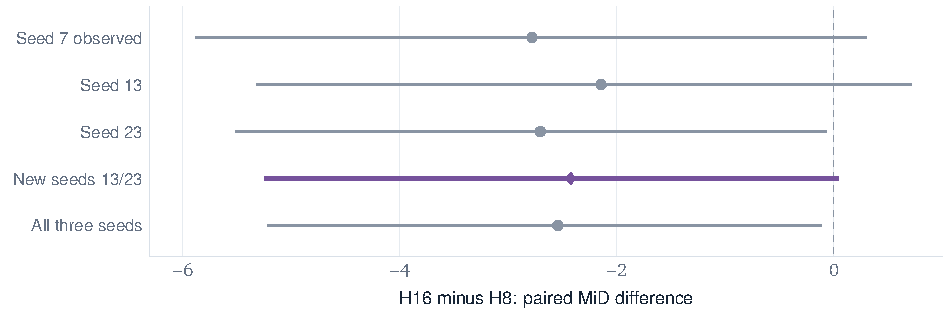
\includegraphics[width=0.98\linewidth]{figures/rev_h16.pdf}
\caption{Paired H16-minus-H8 MiD differences for three head seeds on OLD\_DEV.}
\label{fig:middle-h16}
\end{figure}

The full expert/context model outperformed every registered reduction. FULL-C0 scored 121.4 MiD, versus 127.8 for A5-only, 126.7 for C2F-only, and 124.7 for A5 plus PAIR. Unordered aggregation with age reached 122.4; removing explicit time gave 123.7. Each reduction failed the accuracy screen or its small-excess-error bound. The experts themselves can encode temporal information, so this comparison does not isolate recurrence as the source of the gain. \evidence{M_SIMPLEX}

The analytic EWMA/transport control lost to H8 on every sequence, scoring 155.4 versus 121.6 MiD; the hierarchical interval for the 33.8-point difference was $[17.1,51.0]$. WIDE averaged 119.0 across three head seeds, but its intervals against both H8 and H16 crossed zero. It was not promoted. \evidence{M_EWMA,M_WIDE}

\subsection{Capacity and teacher-feature coverage}

Stage70--76 and the V11 capacity extension planned direct, pairwise-predictive, trajectory, and temporal-permutation comparisons at approximately 2M, 4M, and 8M parameters. The 4M trajectory model was primary. The proposed 30,000-query set covered 27 sequences; extra timestamps increased density, not the number of independent acquisitions.

The V11 audit found teacher features for 4,775 historical tokens and none for the other 25,225. Matching token IDs also left ROI construction, RGB preprocessing, and teacher provenance unresolved. \evidence{M_CAPACITY_PROTOCOL,M_CAPACITY_AUDIT}

Stage70 ended with both completed and unfinished endpoints. The partial record supplies no capacity ranking and no evidence that unlabeled JEPA pretraining improved SIMPLEX-T. \evidence{M_STAGE70_LEDGER}

\section{Transfer, output stability, and runtime}
\label{sec:transfer-context}

\subsection{Development, training, and transfer populations}

The transfer studies answer different questions from OLD\_DEV and TRAIN40. OLD\_DEV had already guided development, and TRAIN40 includes fitted examples. EvTTC and Forward Collision Warning Data (FCWD) instead evaluate frozen models with dataset-specific adapters. FCWD contains three driving sequences with paired events, frames, and LiDAR-derived TTC \citep{eventaided}. The expanded EvTTC set adds timestamps to the same 32 sequences rather than a new holdout.

The earlier H8/TRAIN40 route predates the final refit in Section~\ref{sec:train40}. A5 and C2F each received 49,932 updates, the pair head 6,840, and each of three H8 heads 2,500. Its 88,744 training predictions diagnose fit but cannot estimate unseen-scene performance. Inference used events, while training also used an RGB teacher and geometric supervision. \evidence{M_SCIENCE_AUDIT}

The initial EvTTC evaluation had 946 valid targets among 1,024 queries from 32 sequences; the expansion had 3,640 among 3,947. FCWD contributed 597 eligible targets among 630 queries from three previously exposed sequences. We left rows without ground truth unscored, and all reported methods returned finite predictions on the eligible rows. Full RGB/event Garl was omitted from FCWD because the RGB-to-event mapping had not been verified. \evidence{M_V12_EVTTC_946,M_V12_EVTTC_3640,M_V12_FCWD_597}

\subsection{Input and output conditions}

H8 used retrospective event history and supplied oracle ROI metadata. Garl event-only used its native pair of event windows, while Garl full added RGB. The systems differed in context and input construction. EvTTC projected RGB to events with calibrated rotation but no depth-dependent parallax correction. These transfer adapters do not reproduce the published benchmark protocol.

We corrected RGB synchronization before running full Garl. Selected images had to lie within 1\,ms of each event endpoint and about 100\,ms apart; the largest admitted offset was 453\,$\mu$s. The runner strictly loaded the released checkpoint and upstream normalization. Because we designed the RGB extension after inspecting event-only results, this comparison remains exploratory even though the weights stayed frozen. \evidence{M_TRANSFER_REPORT}

H8 bounds TTC at $\pm60$ seconds. Garl keeps its native scale-ratio division, which emits very large finite values when the estimated scales nearly match. We retained those predictions in the full-population metrics.

\subsection{Transfer results and metric-dependent rankings}

% Generated by research/middle_tables.py; do not edit numeric values.
\begin{table}[tbp]
\centering\small
\caption{Frozen H8 and Garl models evaluated on EvTTC and FCWD.}
\label{tab:middle-transfer}
\setlength{\tabcolsep}{5pt}
\begin{tabular}{lrrrr}
\toprule
Method & MAE (s) & Median AE (s) & RMSE (s) & RTE (\%) \\
\midrule
\multicolumn{5}{l}{\textbf{EvTTC: 946 eligible / 1,024 queries; 32 sequences}} \\
H8 / head 7 & 1.321 & 0.766 & 3.027 & 62.35 \\
H8 / head 13 & 1.353 & 0.731 & 3.206 & 62.92 \\
H8 / head 23 & 1.409 & 0.738 & 3.392 & 68.87 \\
Garl event & 8.048 & 0.997 & 159.247 & 293.47 \\
Garl RGB + event & 1.868 & 0.692 & 7.875 & 76.77 \\
\midrule
\multicolumn{5}{l}{\textbf{EvTTC expanded: 3,640 / 3,947; same 32 sequences}} \\
H8 / head 7 & 1.361 & 0.722 & 3.475 & 53.70 \\
H8 / head 13 & 1.395 & 0.699 & 3.618 & 54.52 \\
H8 / head 23 & 1.456 & 0.702 & 4.003 & 59.15 \\
Garl event & 4.560 & 0.958 & 83.896 & 161.12 \\
Garl RGB + event & 94.510 & 0.661 & 5561.622 & 5180.18 \\
\midrule
\multicolumn{5}{l}{\textbf{FCWD: 597 / 630; three sequences}} \\
H8 / head 7 & 1.778 & 0.675 & 3.588 & 30.20 \\
H8 / head 13 & 1.597 & 0.580 & 3.258 & 27.41 \\
H8 / head 23 & 1.569 & 0.598 & 3.109 & 27.48 \\
Garl event & 2.146 & 0.602 & 5.072 & 26.89 \\
\bottomrule
\end{tabular}
\par\vspace{4pt}
\begin{minipage}{0.98\linewidth}\footnotesize Scores use queries with valid TTC targets; prediction coverage is 100\% on these queries. H8 bounds TTC at $\pm60$\,s, while Garl retains its native signed outputs. The FCWD comparison uses event-only inputs. \evidence{M_V12_EVTTC_946,M_V12_EVTTC_3640,M_V12_FCWD_597}\end{minipage}
\end{table}

H8 had the lowest mean error on the first 946 EvTTC targets: its three heads reached 1.32--1.41 seconds MAE, versus 8.05 for Garl event-only and 1.87 for Garl full. Garl full had the best median, 0.69 seconds versus 0.73--0.77 for H8. \evidence{M_V12_EVTTC_946}

The 3,640-target expansion showed the same split. H8 achieved 1.36--1.46 seconds MAE, Garl event-only 4.56, and Garl full 94.51. Yet Garl full retained the best median at 0.66 seconds, ahead of H8's 0.70--0.72. Rare near-singular scale ratios drove Garl full's mean, so native-output and matched-clipping results remain separate. \evidence{M_V12_EVTTC_3640}

On FCWD, H8 led in MAE at 1.57--1.78 seconds versus 2.15 for Garl event-only. Garl led in mean relative TTC error at 26.9\%, compared with 27.4--30.2\% for H8. These rankings weight the TTC distribution differently, and only three sequences were available for clustered uncertainty. \evidence{M_V12_FCWD_597}

\subsection{Head and full-route runtime}

% Generated by research/middle_tables.py; do not edit numeric values.
\begin{table}[tbp]
\centering\small
\caption{Head-only and full-pipeline runtime.}
\label{tab:middle-cost}
\setlength{\tabcolsep}{5pt}
\begin{tabular}{l@{\hspace{12pt}}r@{\hspace{12pt}}r@{\hspace{12pt}}r@{\hspace{12pt}}r}
\toprule
Model & MiD & Head p95 (ms) & Route 1 p95 (s) & Route 2 p95 (s) \\
\midrule
H1\_SEED7 & 132.832 & 9.28 & 2.944 & 2.902 \\
H8\_SEED7 & 121.646 & 19.47 & 9.349 & 8.479 \\
H16\_SEED7 & 118.866 & 31.45 & 13.201 & 15.304 \\
FULL\_C0 & 121.405 & 21.07 & 8.477 & 9.337 \\
A5\_ONLY\_C0 & 127.785 & 21.42 & 7.928 & 7.471 \\
C2F\_ONLY\_C0 & 126.705 & 19.28 & 8.185 & 8.256 \\
A5\_PAIR\_C0 & 124.669 & 19.83 & 7.086 & 7.502 \\
SET\_AGE\_C0 & 122.443 & 10.00 & 7.628 & 8.303 \\
SET\_NOTIME\_C0 & 123.687 & 9.91 & 7.727 & 7.967 \\
\bottomrule
\end{tabular}
\par\vspace{4pt}
\begin{minipage}{0.98\linewidth}\footnotesize Head: median of three blockwise p95 values, CPU FP32, prepared inputs, 500 measurements per block. Route: p95 on 64 TRAIN queries with supplied ROI, shared GPU, and resident producers. Accuracy uses OLD\_DEV seed 7, nine sequences and three folds. \evidence{M_HEAD_COST,M_ROUTE_COST}\end{minipage}
\end{table}

Prepared-input CPU profiling measured three rotated-order blocks of 500 batch-one calls per head. Median blockwise p95 was 9.28\,ms for H1, 19.47\,ms for H8, and 31.45\,ms for H16. The timer covered canonical TTC emission, but not event reading, ROI construction, expert inference, detection, or tracking. \evidence{M_HEAD_COST}

The shared-GPU route was much slower than the isolated heads. Across 1,728 supplied-ROI requests from 64 TRAIN queries, H8 p95 was 9.35 and 8.48 seconds in two warm blocks; H16 reached 13.20 and 15.30 seconds. The application reopened HDF5 inputs between cold measurements, while the operating system could retain cached pages. \evidence{M_ROUTE_COST}

ROI/voxel reading and preparation consumed 85.5\% of H8's measured time and 90.4\% of H16's in the second warm block. We focused V12 on preparation, bounded caching, and transfer scheduling rather than head speed alone. \evidence{M_ROUTE_REPORT}

CUDA graphs reduced recorded A5 launches from 5,877 to 1,270 while preserving the tested outputs, losses, RNG state, and gradients. A later window measured 41.78 versus 32.89 updates/min, but host load and data wait also changed, so the run did not isolate graph speedup. Adaptive caching reached 26.31 updates/min against a 36.75 reference and failed its throughput test. \evidence{M_ENGINEERING}
\section{From event representations to multimodal measurement}
\label{sec:late}

The later experiments assembled spatial measurement, temporal transport, signed-TTC readout, and multimodal correction into one causal estimator. PHASE-TTC combines task adaptation and teacher supervision with event/RGB producers, context models, and a compact fusion head. No matched factorial separated all of these components, so the final result does not establish a JEPA contribution.

\subsection{V13: a parallel RGB route and a common temporal interface}

V13 added an RGB route with the event branch's A5, C2F, PAIR, and temporal-context decomposition. The common interface made it possible to test event information after an image-based TTC estimate. Each modality still used its own checkpoints, normalization, training data, and temporal support.

Three disjoint acquisition-group roles separated fitting stages. P supplied 53,890 queries from 24 sequences for producers and PAIR. H supplied 18,422 queries from eight sequences for downstream normalizers and heads, while V supplied 16,432 queries from eight sequences for internal evaluation. Earlier work had already used V, so its results remain development evidence.

PHASE17 connected both modalities to their context models through named phase, timing, and support fields. Their meanings remain stable across folds, whereas independently trained encoders can rotate their latent coordinates. The explicit interface enabled grouped out-of-fold training without a separate latent-alignment model.

\subsection{V14: changing the emphasis of the objective}

V14 could not improve short-TTC error without harming other ranges. Its six-cell factorial combined three sample-mass schemes with two losses, holding the frozen event producers, PAIR parent, and seed-7 draws fixed. Each 160-unit, two-layer GRU head received 2,500 updates over eight masked history slots and seventeen features; timestamps represented gaps without dense imputation.

M0 retained the native mass vector. M1 preserved mass per acquisition group while allocating TTC bands in the ratio 0.5/0.3/0.1/0.1. M2 also balanced crucial and long bands, bounding each row between 0.25 and four times its M1 weight. Uniform sampling with replacement kept the number of episodes unchanged. L0 retained the phase, quantile, and auxiliary objectives; L1 added
\begin{equation}
\mathcal L_1=\mathcal L_0+0.25\,\mathbb E_{i\sim\mathrm{batch}}
\left[Nm_i\,\mathrm{SmoothL1}\!\left(
\frac{\widehat T_i-T_i}{\max(|T_i|,0.5\,\mathrm{s})},0\right)\right],
\end{equation}
where $m_i$ is the registered sample mass. Both losses kept the native TTC mapping, clipping, and flat-gradient regions; neither used a straight-through estimator.

\begin{table}[tbp]
\centering\small
\caption{V14 factorial study on exposed V: apparent crucial-range gains can coexist with non-crucial regressions. Source \evidence{L02}.}
\label{tab:late_v14}
\begin{tabular}{lrrrr}
\toprule
\textbf{Model} & \textbf{MiD} & \textbf{Crucial} & \textbf{Negative} & \textbf{MAE (s)} \\
\midrule
RT-M0-L0-S7 & 106.21 & 156.83 & 61.38 & 2.51 \\
RT-M0-L1-S7 & 101.94 & 149.59 & 61.01 & 2.03 \\
RT-M1-L0-S7 & 102.23 & 134.47 & 84.21 & 2.98 \\
RT-M1-L1-S7 & 104.04 & 136.19 & 80.04 & 2.34 \\
RT-M2-L0-S7 & 104.32 & 134.87 & 87.62 & 3.37 \\
RT-M2-L1-S7 & 104.83 & 134.59 & 79.93 & 2.38 \\
\bottomrule
\end{tabular}
\end{table}

Every V14 candidate failed the full gate. M1--L0 reduced crucial-band MiD from 156.8 to 134.5, while large-band error rose from 52.2 to 76.4 and negative-band error from 61.4 to 84.2. M0--L1 achieved the best aggregate and MAE in the matrix, but missed the required crucial-band improvement and other safeguards. All outputs were finite; the failures came from measured regressions. \evidence{L02}

Only 76 V queries fell in the urgent interval $(0.1,1]$ seconds. Across the factorial, 81.6--100\% received late warnings; negative TTC predictions did not count as positive warnings. Such miss rates preclude a safety claim regardless of false-alert rate.

V14 closed as \texttt{NO\_CANDIDATE}, so the conditional replication and transfer stages did not run. The factorial exposed a tradeoff between urgent-range accuracy and the other signed-TTC ranges without producing an admissible improvement.

\begin{figure}[t]
\centering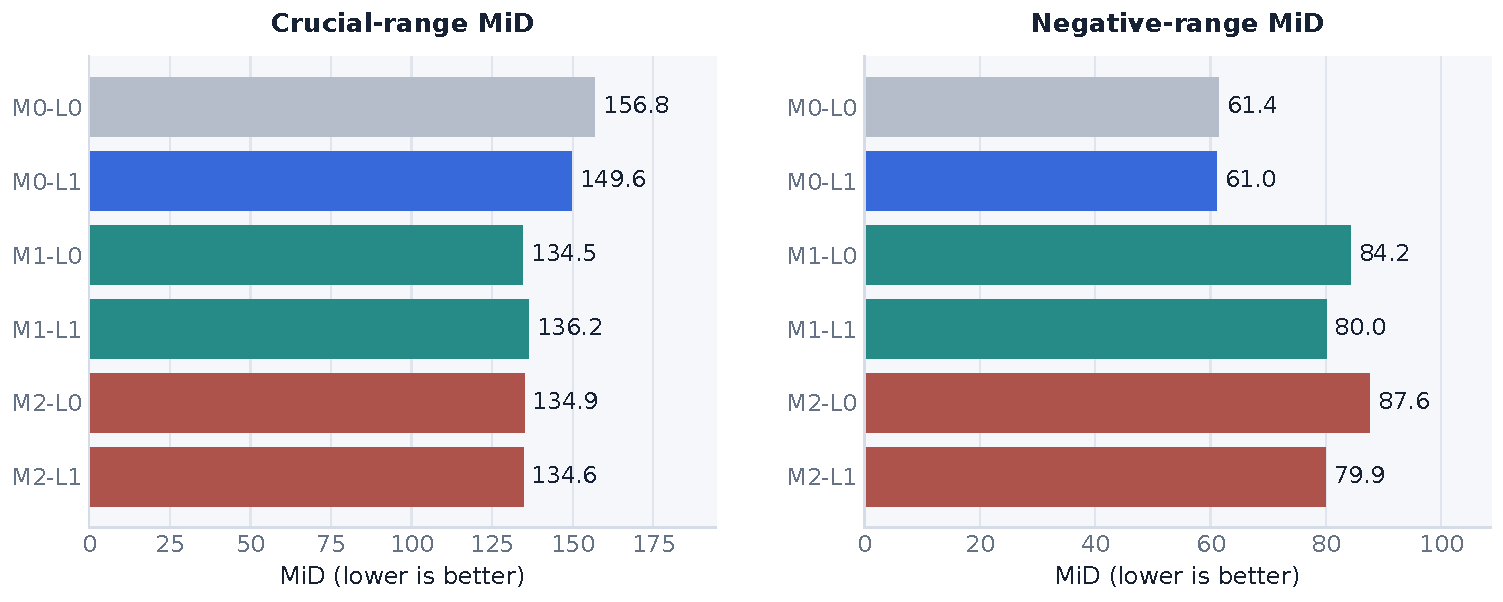
\includegraphics[width=0.98\linewidth]{figures/range_tradeoffs.pdf}
\caption{V14 MiD changes across crucial, small, large, and negative TTC bands.}
\end{figure}

\subsection{V15 and V17: testing readout and geometry explanations}

Neither V15 intervention passed all gates. Sampling proportional to sample mass, corrected by $w_i/p_i$, preserved V14's cross-band tradeoff. Expanding the A5 residual range through an equal-slope hyperbolic tangent left crucial-band performance almost unchanged. The modified producer received regenerated PHASE17 fields and H normalizers.

V17 tested frozen geometry from several angles. A bypass exposed geometry and transport tokens to the temporal head; other arms examined learned NLL precision, grouped ridge probes, directional differences, height calibration and supervision, vertical position, gradient clipping, and nonlinear spatial-height readout. Each had a dedicated control. Directional differences remove static levels while also reducing dimensionality, so they do not isolate appearance memorization.

The geometry bypass carried a useful but unstable downstream signal. On V, its three-seed mean improved crucial MiD from 157.1 to 148.4 and aggregate MiD from 106.5 to 102.8, while MAE worsened. The effect was stronger on H than V, and the three heads shared encoders rather than repeating representation training. \evidence{L50}

The first height-regression arm emitted predictions outside the admissible MiD domain. We kept those rows and left its aggregate missing instead of clipping them away. Temporal supervision restored coverage but not competitive TTC accuracy. Preserving vertical positions improved training height fit while worsening H TTC, and the nonlinear readout also failed. The tested frozen-feature calibration was insufficient, though the bypass result still showed usable geometric signal.

Removing gradient clipping changed little. Learned precision improved crucial-band error in every head seed, but missed the required magnitude and safeguards. The recorded gradient norms describe one loss component rather than the full-dataset objective. None of V17's nine research lines produced a candidate. \evidence{L51,L52}

\subsection{V18: adaptation of the measurement stage}

V18 moved adaptation into the measurement stage. Its primary comparison covered direct and correspondence-based pair readouts, trained and frozen encoders, and a native-system control. C1 tested geometric readout, D1 predictor width, B1 auxiliary correspondence supervision, and A1 adaptation depth. Some arms also updated correspondence, so equal TTC-update counts did not mean equal computation.

C1 improved bandwise geometry over an unconstrained pair-correction readout but failed as a complete TTC estimator. D1 found no benefit from greater predictor width. B1 beat a TTC-only control at the same number of TTC updates, yet its negative-band error blocked promotion over A5. A1 then compared full adaptation with partial retention of the correspondence-trained representation.

A1-FULL delivered V18's largest TTC gain and its clearest tradeoff. On H, aggregate MiD fell from 112.3 for A5-P2 to 78.9, and crucial MiD from 157.3 to 95.8; negative MiD rose from 65.5 to 87.1. It passed the global sign-error safeguard and beat last-block adaptation overall, but did not preserve accurate negative magnitude or demonstrate retention of the correspondence representation. \evidence{L10,L24,L25}

C1 also tested event information after the RGB context estimate. TRUE fusion and an equal-capacity ZERO-event control used seeds 7, 13, and 23. Each seed repeated C1 adaptation and head fitting, while all shared the historical A5 initialization and RGB context parent. The comparison isolates event input within this configuration, not variability from complete pretraining.

TRUE fusion improved on ZERO within V18. Across seeds, aggregate MiD was $87.3\pm0.9$ for TRUE and $92.5\pm0.2$ for ZERO; TRUE's crucial MiD was $126.6\pm0.9$. A paired whole-group bootstrap favored TRUE in aggregate loss. The crucial-band gain missed the preregistered 10\% threshold, and the interval against the preserved V16 PHASE-ONLY family crossed zero at about $[-3.7,0.1]$. Thus, events complemented RGB in this model without establishing superiority over V16. \evidence{L03,L31,L32,L33}

No V18 arm satisfied the complete promotion gate, and the campaign closed as \texttt{NO\_CANDIDATE}. A later portability replay verified archived metrics and exports without adding training or performance evidence.

\begin{table}[tbp]
\centering\small
\caption{V18 primary and adaptive experiments on development subset H (18,422 rows). Sources \evidence{L10--L14,L20--L25}.}
\label{tab:late_v18}
\begin{tabular}{lrrrr}
\toprule
\textbf{Model} & \textbf{MiD} & \textbf{Crucial} & \textbf{Negative} & \textbf{MAE (s)} \\
\midrule
A5-P2-FROZEN & 112.29 & 157.27 & 65.52 & 5.64 \\
PAIR-DIRECT-S7 & 103.87 & 117.98 & 148.17 & 5.00 \\
PAIR-CORR-S7 & 103.51 & 115.56 & 156.00 & 5.50 \\
PAIR-CORR-FROZEN-S7 & 106.72 & 123.61 & 146.99 & 5.40 \\
NATIVE-P2-FT-S7 & 104.05 & 145.12 & 61.26 & 4.65 \\
PAIR-CORR-GEOMETRY-S7 & 90.95 & 114.35 & 106.23 & 6.95 \\
PAIR-CORR-WIDE-S7 & 115.12 & 124.48 & 206.42 & 6.79 \\
B1-TTC-CONTROL-STAGE2-S7 & 85.98 & 106.71 & 96.63 & 6.11 \\
B1-CORRESPONDENCE-STAGE2-S7 & 81.44 & 100.22 & 84.12 & 5.48 \\
A1-LAST-BLOCK-S7 & 90.64 & 111.03 & 97.96 & 7.11 \\
A1-FULL-S7 & 78.92 & 95.85 & 87.09 & 5.45 \\
\bottomrule
\end{tabular}
\end{table}
\begin{table}[tbp]
\centering\small
\caption{V18 C1 equal-capacity TRUE/ZERO event controls on exposed V (16,432 rows), using adaptation/head seeds 7, 13, and 23. Source \evidence{L03}.}
\label{tab:late-fusion}
\begin{tabular}{lrrr}
\toprule
\textbf{Head / seed} & \textbf{Overall MiD} & \textbf{Crucial MiD} & \textbf{MAE (s)} \\
\midrule
FUSION-TRUE-S7 & 88.270 & 127.661 & 1.817 \\
FUSION-ZERO-S7 & 92.638 & 136.989 & 1.842 \\
FUSION-TRUE-S13 & 86.630 & 125.976 & 1.807 \\
FUSION-ZERO-S13 & 92.455 & 136.500 & 1.837 \\
FUSION-TRUE-S23 & 86.961 & 126.069 & 1.818 \\
FUSION-ZERO-S23 & 92.315 & 136.314 & 1.836 \\
\bottomrule
\end{tabular}
\end{table}
\begin{figure}[t]
\centering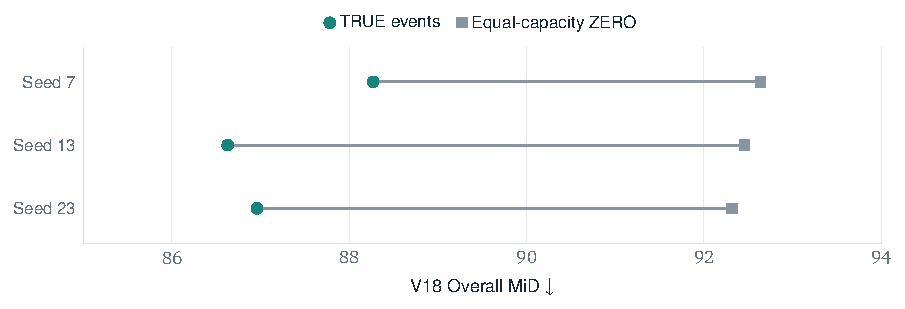
\includegraphics[width=0.98\linewidth]{figures/rev_v18.pdf}
\caption{V18 measurement adaptations and paired TRUE/ZERO event-fusion controls.}
\end{figure}

\subsection{V19: repairing negative motion changes the tradeoff}

V19 tested loss weighting as the source of A1's negative-band regression. L0 and LW shared the correspondence-trained B1 parent, full adaptation, seed 7, uniform sampling, and 12,000 updates. L0 assigned crucial/small/large/negative masses of 50/30/10/10\%. LW doubled negative mass to 20\% and set the positive bands to 44.44/26.67/8.89\%, preserving their relative proportions. The encoder did not change.

\begin{table}[tbp]
\centering\small
\caption{V19 decision recovery on exposed H. LW trades a small overall MiD increase against improved MAE and negative-range behavior. Source \evidence{L30}.}
\label{tab:late_v19}
\begin{tabular}{lrrrr}
\toprule
\textbf{Model} & \textbf{MiD} & \textbf{Crucial} & \textbf{Negative} & \textbf{MAE (s)} \\
\midrule
A5 & 112.29 & 157.27 & 65.52 & 5.64 \\
L0 & 78.92 & 95.85 & 87.09 & 5.45 \\
LW & 79.87 & 100.42 & 70.78 & 4.61 \\
\bottomrule
\end{tabular}
\end{table}

LW repaired part of the negative-motion error but worsened the primary aggregate. Relative to L0, it reduced negative MiD by 18.7\%, MAE by 15.3\%, and sign error by 1.55 percentage points, while aggregate and crucial MiD increased. The same pattern appeared on P training data, ruling out an H-only generalization failure. Because the replication trigger required lower aggregate error, LW did not advance. \evidence{L30}

Later two-expert selectors also failed the system gate. They required both fitted experts and the measured feature path, rather than forming a jointly trained sparse mixture. Grouped validation limited fitting leakage, while reused H data and fixed experts constrained the conclusion to these selectors.
\FloatBarrier
\section{Experimental chronology}
\label{sec:history}

Development began in June 2026 with the E-JEPA-TTC hypothesis: predictive latent
learning might improve event-based TTC estimation. The research then moved
through geometry and cross-time transport to temporal context and RGB--event
fusion. Several evaluation corrections changed which results could support a
claim.

\subsection{June--July: predictive learning and evaluation corrections}

The first experiments established indexed EvTTC access, voxel representations,
a TinyCNN, and geometric/event-rate baselines. JEPA pretraining with
latent-variance regularization led to multihorizon prediction, frozen-encoder
probes, and low-label comparisons. Token transformers, tubelets, deep token
supervision, navigation conditioning, and rollout probes tested other forms of
temporal information.

Centered derivatives gave the geometric baseline access to future observations.
We replaced them with past-only derivatives and reported this annotation-assisted
baseline on its supported queries, separate from models with different inputs or
coverage.

On 13 July, we reclassified the inspected CPLA-high results as reused-test
diagnostics (\texttt{26480260}). Their three fine-tuning seeds shared one SSL
initialization, so the spread reflects downstream optimization conditional on
that parent. We removed the runs from final-test claims and added checkpoint,
cache-version, nested-subset, and matched-scratch checks. No repartition of the
inspected sequences could recreate a blind holdout.

An eAP smoke-validation defect wrote success markers without running the matrix
(\texttt{1f9e2f99}). We replaced the faulty path with the matrix invocation and
added a regression test; the old markers were discarded as evidence.

\subsection{August: geometry, transport and fold-local parents}

August introduced physics-constrained FlowMimic, dense LevelDynamics,
object-centric representations, and matched Garl comparisons. The A-series
varied foreground geometry and decoder capacity, then added SAM supervision and
DINOv3 relational distillation. A4 used an RGB teacher; A5 learned local
cross-time transport on disjoint training rows. These stages no longer tested
the original label-free JEPA objective alone.

On 13 August, we found that several grouped runs inherited an A4 parent trained
on their held-out outer groups (\texttt{de3349fd}). Those summaries remain
parent-exposed diagnostics. The corrected study trained A4 inside each outer
fold, keeping the held-out group out of both representation learning and
downstream fitting.

V6 and V7 produced no promoted model. A post-hoc A5/C2F routing result from V7
became a prospective V8 hypothesis. V8 then tested temporal mechanisms and
nested routing after correcting ROI quantization, timestamp bins, and bounded
HDF5 reads. Unsupported predictions stayed in the evaluation as named failures.

\subsection{September--October: context and multimodal measurement}

X0/X1 and Stages 61--76 tested phase dynamics, raw timing, routing, risk, and
context under fixed optimization budgets. Nested producers excluded held-out
groups from training, and incomplete runs were not promoted to completed
evaluations.

SIMPLEX-T completed 24 head fits and 60,000 updates. Its H8/H16 comparisons
retrained heads while sharing upstream producers. Efficient-context work then
addressed TRAIN40 inputs and execution cost; the RGB port added native sensor
clocks and transfer studies. The record also retains failed geometry, clipping,
and nonlinear-readout controls from the range and representation studies.

The multimodal V16 phase-correction family supplied the final-refit recipe.
V18 tested joint measurement, correspondence, geometric readout, predictor
capacity, and encoder adaptation. Some arms improved individual bands, but none
passed every promotion criterion; V18 closed as \texttt{NO\_CANDIDATE}. V19
then tested negative-loss weighting and fixed expert selection.

\subsection{October: final refit and causal runtime}

The final TRAIN40 refit used group-separated auxiliary producers for
out-of-fold inputs and full-TRAIN40 producers for deployment. It followed the
V16 recipe but trained a new model lineage. The submission preserved query-token
identity and complete prediction coverage, and its official score placed
PHASE-TTC first on the public GarlTTC Test leaderboard on 28 October 2026
(Section~\ref{sec:official}).

Runtime experiments covered persistent histories, exact normalization, graph
execution, crop reuse, and multiobject replay. Timing reports separated startup
from measured arrivals and counted valid TTC outputs separately from failed acknowledgements.
The 5\,ms ingestion experiment kept 20\,ms output queries and established
numerical parity for that setting; it did not measure throughput.
\section{Reproducibility}
\label{app:reproduction}

The release contains the manuscript source, analysis scripts, derived-result
ledgers, and selected query-level predictions needed to regenerate the reported
tables and figures. Repeating model training or sensor inference also requires
the datasets, checkpoints, and experiment configurations listed in the evidence
registry.

\subsection{Manuscript and result regeneration}

Install Python, NumPy, Matplotlib, and a LaTeX distribution. From the manuscript
source root, run:
\begin{lstlisting}
python scripts/build_final.py
\end{lstlisting}
The script verifies the distributed files, regenerates figures and tables, and
runs pdfLaTeX, BibTeX, and the required cross-reference passes. Once the
dependencies are installed, the build uses bundled ledgers and requires neither
network access nor raw sensor data.

Each ledger records the evaluation population, source key, and measured value.
The verification scripts match source identities and recompute metrics from the
distributed query-level predictions. Hardware-specific inference parity requires
the corresponding checkpoints, inputs, and runtime environment.

\subsection{Numerical verification}
The verification suite checks 13 data-file hashes, eight transfer summaries, twelve official-scorer fields, and weighted Overall MiD. The competition verifier recomputes coverage, signed ranges, disagreements, and timing summaries from all 1,736 model--query rows. The dated leaderboard snapshot supplies the official ranking.

\begin{table}[H]
\centering\small
\caption{Additive decomposition of the official Overall MiD difference. Each band contributes $w_b(\mathrm{MiD}^{\mathrm{Garl}}_b-\mathrm{MiD}^{\mathrm{PHASE}}_b)$. The 0.0010-point reconciliation residual comes from Garl-TTC's published two-decimal band scores and appears separately below. \evidence{B01,B02}}
\label{tab:official-weighted-contributions}
\begin{tabular}{lrrr}
\toprule
\textbf{Band} & \textbf{Weight} & \textbf{MiD difference} & \textbf{Weighted contribution} \\
\midrule
Crucial & 0.5 & 9.6110 & 4.8055 \\
Small & 0.3 & 9.3232 & 2.7970 \\
Large & 0.1 & 14.8921 & 1.4892 \\
Negative & 0.1 & 1.3586 & 0.1359 \\
\midrule
Band subtotal & 1.0 & -- & 9.227548419 \\ 
Published-score rounding residual & -- & -- & 0.0010 \\ 
Official Overall difference & -- & -- & 9.228548419 \\ 
\bottomrule
\end{tabular}
\end{table}

The transfer analysis recomputes mean, median, p95, and relative error for four Extended-new methods from 468 eligible rows. It then constructs error-exceedance curves and paired complete-sequence bootstrap intervals. The fixed seed, quantile convention, bootstrap differences, and source-file digest reside under \path{revision/}. This post-hoc analysis uses fixed predictions and does not repeat model training or inference.

\subsection{Paced-run configuration}
The L40 receipts identify the final model and component digests used for the PHASE-TTC competition inference, while recording a separate replay input and timing protocol. Synthetic startup priming used no raw observations or targets and made no optimizer updates. The update clock includes unexpected shape preparation. The receipts omit the CPU model and GPU-driver version. \evidence{L40,R02}
\begin{table}[H]\centering\small
\caption{Paced-replay hardware, configuration, and initialization timings. Startup stages were timed separately and excluded from the arrival clock; unexpected shapes were processed within the measured update. \evidence{L40,R02}}
\label{tab:runtime-setup}
\begin{tabularx}{\linewidth}{@{}p{.31\linewidth}X@{}}\toprule
Item & Recorded value\\\midrule
GPU & NVIDIA GeForce RTX 5070 Ti Laptop GPU\\
Software & Python 3.11.15; PyTorch 2.11.0+cu128; CUDA build 12.8\\
Precision & FP32; TF32 disabled for matrix multiplication and cuDNN\\
CPU / preparation & 2 PyTorch CPU threads; 8 RGB workers; queue capacity 2\\
Parity tolerance & Absolute and relative tolerance both $10^{-5}$; all 250 outputs checked\\
\midrule\multicolumn{2}{l}{\textbf{Outside the measured arrival clock}}\\
RAW preload & 2.769 s\\
Model and service initialization & 0.516 s\\
Synthetic shape priming & 12.095 s; 7 layouts; synthetic tensors only, no RAW/future sensor data\\
History initialization & 0.132 s for 600 ms of preceding sensor history\\
Source warmup & 0.051 s; 13 already-available RGB frames\\
\midrule
Unrecorded hardware fields & CPU model and GPU driver version\\
\bottomrule\end{tabularx}\end{table}

\subsection{Code verification}

Selected tests cover event representations, target updates, prefix causality,
label rejection, source tracking, fusion fallbacks, and paced-runtime accounting.
The environment used Python 3.11.15, PyTorch 2.11.0+cu128, and pytest 9.1.1.
Across two batches, 178 tests passed and four skipped, with no failures. Four
additional tests ran against the SHA-pinned official evaluator and passed with
no skips or failures. They cover perfect predictions across four bands,
crucial-band weighting, absent-band handling, and invalid-output retention.
\evidence{M21,M24}

For the competition adapter and verifier, 41 focused tests passed; the
CPU-oriented suite skipped one conditional CUDA case. A separate CUDA test
confirmed strict loading and native-model forward parity for all three public
Garl checkpoints. Post-run validation covered 1,302 Garl terminal records, 434
PHASE predictions, input identities, causal timing, signed FP32 height-ratio
conversion, and complete or partial result packages. \evidence{T01}

\subsection{Evidence integrity and source revision}

SHA-256 checks identify 95 original result snapshots.
Appendix~\ref{app:evidence} lists their digest prefixes and numerical projections.
Entries without a projection preserve source identity but cannot support metric
recomputation from the distributed data alone. For the official benchmark, the
scorer JSON agrees with the dated leaderboard after display rounding. Because
the scorer output contains no submitted-prediction hash, it does not link the
reported score to a specific prediction file at the byte level.

The scientific source snapshot is
\path{0219a84f0fc3b07c171295a8a65176a7e0f631c1} in
\href{https://github.com/Kripta-Studios/phase-ttc}{Kripta-Studios/phase-ttc}.

The competition adapter used source revision
\path{1d8de7d95b2ff8ccba884dbd40141c48745a1e95}. The public competition
projection contains the numerical predictions, measurement boundaries,
checkpoint identities, and source digests required to regenerate coverage,
disagreement, and timing summaries without distributing raw sensor files.

\path{ASSETS.md} documents the supplied visual material and its attribution.
The visual-source manifest records the sensor illustration's checksum and
transformation; original dataset and material rights remain with their owners.
\section{Evidence index}
\label{app:evidence}
Source keys map each reported measurement to its result artifact. Numerical ledgers drive table and figure regeneration, while \path{data/public_evidence_registry.json} records full digests and field selectors. The index separates original-artifact hashes from distributed-file hashes. \emph{Digest only} entries preserve source identity without distributing the fields required for metric recomputation. B02 denotes the official scorer JSON.
\subsection{Result-source identities}
\begingroup\footnotesize
\setlength{\tabcolsep}{3pt}
\renewcommand{\arraystretch}{1.08}
\begin{longtable}{@{}>{\raggedright\arraybackslash}p{.32\linewidth}>{\raggedright\arraybackslash}p{.41\linewidth}>{\raggedright\arraybackslash}p{.22\linewidth}@{}}
\toprule
Source key & Distributed ledger & Original SHA-256 \\
\midrule\endfirsthead
\toprule
Source key & Distributed ledger & Original SHA-256 \\
\midrule\endhead
\midrule\multicolumn{3}{r}{\scriptsize Continued on next page}\\\endfoot
\bottomrule\endlastfoot
\path{E01} & \path{data/early_results.json} & \path{55b5494b40f97f1b} \\
\path{E02} & \path{data/early_results.json} & \path{27ee1c9a21cca0ec} \\
\path{E03} & \path{data/early_results.json} & \path{aa46f6d199bcf5a4} \\
\path{E04} & \path{data/early_results.json} & \path{02c215aa4678f307} \\
\path{E05} & \emph{Digest only} & \path{6fe8c8761d0a14fb} \\
\path{E06} & \emph{Digest only} & \path{d38021db5b3b5b62} \\
\path{E07} & \path{data/early_results.json} & \path{d53b6ce406fa7b80} \\
\path{E08} & \path{data/early_results.json} & \path{d69f8b9082c883da} \\
\path{E09} & \path{data/early_results.json} & \path{9bf197c3d64635a3} \\
\path{E10} & \path{data/early_results.json} & \path{d47face1e36d1d2c} \\
\path{E11} & \path{data/early_results.json} & \path{6db419fd7c7fe536} \\
\path{E12} & \path{data/early_results.json} & \path{f33dc9abbad8fd08} \\
\path{E13} & \emph{Digest only} & \path{ac26c1b2ad87c6c9} \\
\path{E14} & \emph{Digest only} & \path{f947b32f05e655a1} \\
\path{E15} & \emph{Digest only} & \path{7c60bc0fa9f1c5f0} \\
\path{E16} & \path{data/early_results.json} & \path{be5fdbc0b2e9773d} \\
\path{E17} & \path{data/early_results.json} & \path{d3fb5a5feb848ac7} \\
\path{E18} & \path{data/early_results.json} & \path{a3c4765f5278a3f4} \\
\path{E19} & \path{data/early_results.json} & \path{f1471599d502f2de} \\
\path{E20} & \path{data/early_results.json} & \path{3e02fd81751e3f86} \\
\path{E21} & \path{data/early_results.json} & \path{5c7b1eb24c07bd08} \\
\path{E22} & \emph{Digest only} & \path{2e2eef6698ef28a4} \\
\path{E23} & \path{data/early_results.json} & \path{bc540cc21ddb317f} \\
\path{E24} & \emph{Digest only} & \path{dab563a02450abe6} \\
\path{E25} & \path{data/early_results.json} & \path{06619299d1ceb785} \\
\path{E26} & \path{data/early_results.json} & \path{06dc45cf3ea7a3e0} \\
\path{M_SIMPLEX} & \path{data/middle_results.json} & \path{93f83e71f86dfcad} \\
\path{M_HEAD_COST} & \path{data/middle_results.json} & \path{8d96bbc9bd66d8fb} \\
\path{M_ROUTE_COST} & \path{data/middle_results.json} & \path{d1d834ab36d14fbd} \\
\path{M_WIDE} & \emph{Digest only} & \path{c15e32a8dea0eece} \\
\path{M_EWMA} & \emph{Digest only} & \path{47cca03ccda6f054} \\
\path{M_STAGE61} & \path{data/middle_results.json} & \path{20f1990bb70e5de7} \\
\path{M_STAGE62} & \path{data/middle_results.json} & \path{c4a0e1ae20d79094} \\
\path{M_GEOMETRY} & \emph{Digest only} & \path{fa917902b5696e4b} \\
\path{M_STAGE67_DECISION} & \emph{Digest only} & \path{ab1d3095955477f4} \\
\path{M_STAGE69_DECISION} & \emph{Digest only} & \path{dfd1956775492584} \\
\path{M_ENGINEERING} & \emph{Digest only} & \path{e756ba5c7a433efd} \\
\path{M_SCIENCE_AUDIT} & \emph{Digest only} & \path{06073f4182de1a41} \\
\path{M_STAGE63_REPAIR} & \emph{Digest only} & \path{f96b7fe795637cc5} \\
\path{M_CAPACITY_PROTOCOL} & \emph{Digest only} & \path{1be3a4c9f9b64a08} \\
\path{M_CAPACITY_AUDIT} & \emph{Digest only} & \path{07ef97a56b4159fa} \\
\path{M_STAGE70_LEDGER} & \emph{Digest only} & \path{62597e162571def0} \\
\path{M_TRANSFER_REPORT} & \emph{Digest only} & \path{d92c9074516354bd} \\
\path{M_ROUTE_REPORT} & \emph{Digest only} & \path{1f29a459c91f6b68} \\
\path{M_TEMPORAL_MODEL} & \emph{Digest only} & \path{4c26ad5ecf9e8354} \\
\path{M_PHASE_CONTRACT} & \emph{Digest only} & \path{7ee447190ef7b218} \\
\path{M_STAGE64} & \emph{Digest only} & \path{68409fb88499899f} \\
\path{M_X0} & \emph{Digest only} & \path{61d8a0e40b6d87ad} \\
\path{M_X05} & \emph{Digest only} & \path{c4aa55dd6a944d01} \\
\path{M_X05_GATE} & \emph{Digest only} & \path{61eae7d38fb6ea5a} \\
\path{M_STAGE65} & \emph{Digest only} & \path{4f88f676eecc7e90} \\
\path{M_STAGE67_DIAGNOSTICS} & \emph{Digest only} & \path{885ac3604160cf27} \\
\path{M_S67_SIMPLEX17} & \emph{Digest only} & \path{969cf5db29b2a251} \\
\path{M_S67_UNCONSTRAINED17} & \emph{Digest only} & \path{1419522be60fc952} \\
\path{M_S67_SIMPLEX8GATE} & \emph{Digest only} & \path{e094512164179869} \\
\path{M_S67_SIMPLEX17_PAIRPERM} & \emph{Digest only} & \path{451821bb98c1d0c2} \\
\path{M_S65_RISK17} & \emph{Digest only} & \path{b964e12180efbcbc} \\
\path{M_S65_RISK8} & \emph{Digest only} & \path{75d98c9e0be9ddc3} \\
\path{M_V12_EVTTC_946} & \path{data/middle_results.json} & \path{03c57b4503ca95f4} \\
\path{M_V12_EVTTC_946_PAIRED} & \emph{Digest only} & \path{5fee507ffe8a4aca} \\
\path{M_V12_EVTTC_946_ROWS} & \emph{Digest only} & \path{d284e52a0c25a897} \\
\path{M_V12_EVTTC_3640} & \path{data/middle_results.json} & \path{792a5042dfa8be8b} \\
\path{M_V12_EVTTC_3640_PAIRED} & \emph{Digest only} & \path{2619cc3d11be7320} \\
\path{M_V12_EVTTC_3640_ROWS} & \emph{Digest only} & \path{20f58c1200b3834d} \\
\path{M_V12_FCWD_597} & \path{data/middle_results.json} & \path{a1c0c4a741b08a36} \\
\path{M_V12_FCWD_597_PAIRED} & \emph{Digest only} & \path{2581bd042f29a466} \\
\path{M_V12_FCWD_597_ROWS} & \emph{Digest only} & \path{68f4cd5610f50c8b} \\
\path{L01} & \path{data/late_results.json} & \path{9136babd4a07411e} \\
\path{L02} & \path{data/late_results.json} & \path{844e0771bab79717} \\
\path{L03} & \path{data/late_results.json} & \path{4af996900a99c585} \\
\path{L10} & \path{data/late_results.json} & \path{f5bf12b2873a2ee4} \\
\path{L11} & \path{data/late_results.json} & \path{22e82a376b18c9f0} \\
\path{L12} & \path{data/late_results.json} & \path{fafd9cefbeddcd49} \\
\path{L13} & \path{data/late_results.json} & \path{86ce201ca25bcc12} \\
\path{L14} & \path{data/late_results.json} & \path{0588956e96dab44f} \\
\path{L20} & \path{data/late_results.json} & \path{6d15d1acfad38592} \\
\path{L21} & \path{data/late_results.json} & \path{2b33ba213186f3c5} \\
\path{L22} & \path{data/late_results.json} & \path{b1ad71b126b20e87} \\
\path{L23} & \path{data/late_results.json} & \path{0698e433731da0d3} \\
\path{L24} & \path{data/late_results.json} & \path{5f3789bd7efebce3} \\
\path{L25} & \path{data/late_results.json} & \path{774c751e4aaa91d7} \\
\path{L30} & \path{data/late_results.json} & \path{1073ab21e307ae26} \\
\path{L31} & \path{data/late_results.json} & \path{54ebca7a19d5a9eb} \\
\path{L32} & \path{data/late_results.json} & \path{d4fbc7494769a5d1} \\
\path{L33} & \path{data/late_results.json} & \path{025a058d846a7ceb} \\
\path{L40} & \path{data/late_results.json} & \path{c27d5d980f2bb1c1} \\
\path{L41} & \emph{Digest only} & \path{d8df9ca6444c6dc0} \\
\path{L42} & \emph{Digest only} & \path{06ab49e521db7255} \\
\path{L43} & \emph{Digest only} & \path{aed0bdd40c58d827} \\
\path{L44} & \emph{Digest only} & \path{e447c5147e4e1c25} \\
\path{L45} & \emph{Digest only} & \path{4f643a15cbf3d963} \\
\path{L46} & \path{data/transfer_queries.csv} & \path{1fbff40f000c879b} \\
\path{L50} & \emph{Digest only} & \path{3069072fb5180272} \\
\path{L51} & \emph{Digest only} & \path{ad4a2a0660bd2da9} \\
\path{L52} & \emph{Digest only} & \path{46e5516c40511837} \\
\path{B01} & \path{data/official_benchmark.json} & \path{0c7114c5acfded5e} \\
\path{B02} & \path{data/official_scoring_scores.json} & \path{e06e99ba1e5d6c4e} \\
\path{T01} & \path{data/evttc_competition_summary.json} & \path{96c849f29383c35f} \\
\path{T02} & \path{data/evttc_competition_summary.json} & \path{ceb5c6b5f3ef1b93} \\
\end{longtable}
\endgroup
\subsection{Implementation and verification references}
Implementation keys map source revisions, method descriptions, and selected verification results to their distributed manifests.
\begingroup\footnotesize
\setlength{\tabcolsep}{3pt}
\renewcommand{\arraystretch}{1.08}
\begin{longtable}{@{}>{\raggedright\arraybackslash}p{.32\linewidth}>{\raggedright\arraybackslash}p{.41\linewidth}>{\raggedright\arraybackslash}p{.22\linewidth}@{}}
\toprule
Source key & Distributed manifest & Ledger selector \\
\midrule\endfirsthead
\toprule
Source key & Distributed manifest & Ledger selector \\
\midrule\endhead
\midrule\multicolumn{3}{r}{\scriptsize Continued on next page}\\\endfoot
\bottomrule\endlastfoot
\path{M01} & \path{research/architecture_sources.json} & \path{id=M01} \\
\path{M02} & \path{research/architecture_sources.json} & \path{id=M02} \\
\path{M03} & \path{research/architecture_sources.json} & \path{id=M03} \\
\path{M04} & \path{research/architecture_sources.json} & \path{id=M04} \\
\path{M05} & \path{research/architecture_sources.json} & \path{id=M05} \\
\path{M06} & \path{research/architecture_sources.json} & \path{id=M06} \\
\path{M07} & \path{research/architecture_sources.json} & \path{id=M07} \\
\path{M08} & \path{research/architecture_sources.json} & \path{id=M08} \\
\path{M09} & \path{research/architecture_sources.json} & \path{id=M09} \\
\path{M10} & \path{research/architecture_sources.json} & \path{id=M10} \\
\path{M11} & \path{research/architecture_sources.json} & \path{id=M11} \\
\path{M12} & \path{research/architecture_sources.json} & \path{id=M12} \\
\path{M13} & \path{research/architecture_sources.json} & \path{id=M13} \\
\path{M14} & \path{research/architecture_sources.json} & \path{id=M14} \\
\path{M15} & \path{research/architecture_sources.json} & \path{id=M15} \\
\path{M16} & \path{research/architecture_sources.json} & \path{id=M16} \\
\path{M17} & \path{research/architecture_sources.json} & \path{id=M17} \\
\path{M18} & \path{research/architecture_sources.json} & \path{id=M18} \\
\path{M19} & \path{research/architecture_sources.json} & \path{id=M19} \\
\path{M20} & \path{research/architecture_sources.json} & \path{id=M20} \\
\path{M21} & \path{research/architecture_sources.json} & \path{id=M21} \\
\path{M22} & \path{research/architecture_sources.json} & \path{id=M22} \\
\path{M23} & \path{research/architecture_sources.json} & \path{id=M23} \\
\path{M24} & \path{research/architecture_sources.json} & \path{id=M24} \\
\end{longtable}
\endgroup
\needspace{14\baselineskip}
\subsection{Distributed data integrity}
Digest prefixes identify the numerical files and manifests used for regeneration; the build verifies each full hash before analysis.
\begingroup\footnotesize
\setlength{\tabcolsep}{3pt}
\renewcommand{\arraystretch}{1.08}
\begin{longtable}{@{}>{\raggedright\arraybackslash}p{.32\linewidth}>{\raggedright\arraybackslash}p{.41\linewidth}>{\raggedright\arraybackslash}p{.22\linewidth}@{}}
\toprule
File ID & Distributed file & SHA-256 prefix \\
\midrule\endfirsthead
\toprule
File ID & Distributed file & SHA-256 prefix \\
\midrule\endhead
\midrule\multicolumn{3}{r}{\scriptsize Continued on next page}\\\endfoot
\bottomrule\endlastfoot
D01 & \path{data/early_results.json} & \path{bbc3e4b30c44e6af} \\
D02 & \path{data/early_tables.json} & \path{e7c769877f14ecf2} \\
D03 & \path{data/git_summary.json} & \path{40b8eac8566ed3de} \\
D04 & \path{data/late_results.json} & \path{e7093f1b75a4e96b} \\
D05 & \path{data/middle_results.json} & \path{236eb5dab7db1932} \\
D06 & \path{data/official_benchmark.json} & \path{f7bc1a8bd786f814} \\
D07 & \path{data/official_scorer_verification.json} & \path{98ccc01371304d3a} \\
D08 & \path{data/official_scoring_scores.json} & \path{e06e99ba1e5d6c4e} \\
D09 & \path{data/transfer_queries.csv} & \path{2fd4c33716a6c48e} \\
D10 & \path{data/visual_source_manifest.json} & \path{7cd53750ff473479} \\
D11 & \path{research/architecture_sources.json} & \path{a544f7aab9d12e34} \\
D12 & \path{data/evttc_competition_summary.json} & \path{9ad728d4168c0b41} \\
D13 & \path{data/evttc_competition_predictions.csv} & \path{5e58c4155d90cf5e} \\
\end{longtable}
\endgroup

\subsection{Post-hoc paired transfer analysis}
R01 maps \path{revision/derived_transfer_analysis.json} and the complete paired-bootstrap differences to \path{scripts/prepare_revision.py}. The analysis uses the L46 transfer-query predictions and retains their source digest. Appendix~\ref{app:derived-transfer} gives the sequence-resampling procedure and numerical cases.

\subsection{Deployment metadata and output map}
R02 maps \path{revision/deployment_contract.json} to the native phase-output transformation and L40 paced-run configuration. It records original source digests, the executed code revision, model identities, hardware, precision, and initialization boundaries. R02 contains metadata from the recorded run rather than a new performance measurement. The build verifies its full digest before regenerating Table~\ref{tab:runtime-setup}.
\end{document}
